\section[Adaptive dynamics]{Adaptive dynamics: Can actions of accreted globular clusters constrain the gravitational potential?}\label{sec:Dynamics}

\subsection{Integrals of motion}\label{subsec:IoMs}
This Section is based on \S3.1, \S3.2 and \S3.5 of \citet{Binney...Tremaine...2008}. Objects (e.g., stars and \acp{GC}) in gravitational potential move on orbits which are described by their positions and velocities in 6 dimensional phase space, (\textbf{x}, \textbf{v}). Functions $I$, which are constant along an orbit, are called \acf{IoM} \citep{Binney...Tremaine...2008}:
\begin{equation}
    I[\mathbf{x}(t_1), \mathbf{v}(t_1)] = I[\mathbf{x}(t_2), \mathbf{v}(t_2)]
\end{equation}
for any $t_1$ and $t_2$. This means, that the time derivative of these \ac{IoM} is 0:
\begin{equation}\label{eq:der_IoM}
    0 = \dot{I}
\end{equation}
In an axisymmetric 3D potential as we assumed and fitted in Section \ref{sec:Auriga} orbits can have up to three \ac{IoM}. 
\subsubsection{Energy and angular momentum}
Energy E and some components of the angular momentum \textbf{L}, depending on the symmetry of the potential, are regarded as classical \ac{IoM}. In a spherical potential, all three components of $\textbf{L} = \textbf{x} \times \textbf{v}$ are \ac{IoM} while in the axisymmetric potential $\Phi$, the only component of the angular momentum which is an integral of motion is $L_z$, i.e. the component aligned with the symmetry. The energy is given by the Hamiltonian H,
\begin{equation}\label{eq:energy_hamiltonian}
    H(\mathbf{x, v}) = \frac{1}{2}v^2 + \Phi(\mathbf{x}) = E
\end{equation}
with the total velocity $v$. In an axisymmetric potential, the \ac{IoM} ($E,L_z$) are supplemented by a third integral of motion, $I_3 =$ constant, which, in general, does not have an analytic expression and therefore is a non-classical integral. 
\subsubsection{Actions}\label{subsubsec:actions_theo}
\textbf{General introduction to actions} A particular set of \ac{IoM} are actions which, together with angles, create a canonical coordinate system. These actions are three momenta, $\mathbf{J} = (J_1, J_2, J_3)$, which describe the whole orbit while the angles, $\bm{\theta} = (\theta_1, \theta_2, \theta_3) $ define the position of the object on the orbit. Orbits for which actions can be calculated are called regular orbits. The three actions are given by the integral
\begin{equation}
    J_i = \frac{1}{2\pi}\oint_{\gamma_i}\mathbf{p}\cdot\mathrm{d}\mathbf{q} \qquad i = 1,2,3
\end{equation}
over the path $\gamma_i$ with vector $\mathbf{q}(t)$ and corresponding momentum $\mathbf{p}(t)$ given a Hamiltonian system which satisfies 
\begin{equation}
    \dot{\mathbf{q}} = \frac{\partial H}{\partial \mathbf{p}} \quad;\quad \dot{\mathbf{p}} = - \frac{\partial H}{\partial \mathbf{q}}. 
\end{equation}
The range of the angles is by construction $\theta_i = [0,2\pi]$ so that it moves periodically around the center of the galaxy. Since $0 = \dot{J} = -\partial H / \partial\theta_i$ (Equation \ref{eq:der_IoM}), the Hamiltonian is independent of $\bm{\theta}$. Therefore, angles follow the time evolution
\begin{equation}
    \dot{\theta}_i = \frac{\partial H}{\partial J_i} \equiv \Omega_i(\mathbf{J}), \quad \mathrm{a\ constant} \quad \Rightarrow\quad \theta_i(t) = \theta_i(0) +  \Omega_i t
\end{equation}
with the fundamental frequencies $\Omega_i$. The components of $\bm{\theta}$ evolve linearly in time. 
\\\\\textbf{Definition in cylindrical coordinates} In the axisymmetric potential we have the spatial coordinates $(R, \phi, z)$ and velocities $(v_R, v_\phi, v_z)$ which we can use for the planes ($x_i, v_i$) in which we examine the actions $\mathbf{J} = (J_R, J_\phi = L_z, J_z)$. The actions quantify the oscillation of the orbit in the given coordinate direction. $J_R$ describes how the object moves towards and away from the galactic center, the radial oscillation, and $J_z$ the oscillation above and below the equatorial plane while $J_\phi = L_z$ is the angular momentum along the symmetry axis. Circular orbits do not oscillate in $R$ and $z$ so the actions in these directions are ($J_R, J_z$) = 0.

\textbf{Numerical calculation of actions} Only in a simple spherical symmetric potential, the Isochrone potential $\Phi(r) = -GM/(b + \sqrt{b^2+r^2})$ with scale length $b$, actions can be calculated analytically without at single integration. To numerically calculate the actions of objects in our axisymmetric potential from Section \ref{sec:Auriga}, we need to use approximations. 
With the motions $(u,v)$ defined by 
\begin{equation}
    R = \Delta \sinh{u} \sin{v}\quad ; \quad z = \Delta \cosh{u}\cos{v}
\end{equation}
and their canonical conjugate momenta $p_u(u, E, L_z, I_3)$ and $p_v(v,E,L_z,I_3$ we can transform the Hamiltonian:
\begin{equation}\label{eq:Ham_trafo}
    H(R,z,p_R,p_z) \Rightarrow H(u,v,p_u, p_v).
\end{equation}
Under the assumption of \textit{separable} St\"ackel potentials \citep{deZeeuw...Staeckel..1985} which have the form
\begin{equation}\label{eq:Stackel_pot}
    \Phi(u,v) = \frac{U(u)-V(v)}{\sinh^2u + \sin^2v}
\end{equation}
we can solve the Hamilton-Jacobi equation by the \textit{separation of variables} ansatz to decouple the motions in $u$ and $v$. Then, both sides of the equation are constant. By clever choice, this constant depends on the third integral of motion, $I_3$ and on the focal length $\Delta$ which defines the coordinate system. The resulting actions $J_u$ and $J_v$ depend on the three computable actions $(E, L_z, I_3$), the focal length $\Delta$ and on the St\"ackel potential but need only one integral to solve instead of an orbit integration. The cylindrical actions are $J_R \approx J_u$ and $J_z \approx J_v$. The St\"ackel Fudge method \citep{Binney...StaeckelFudge...2012, Bovy...actionbasedmodelling...2013}, just pretends that the given potential is a St\"ackel potential. The closer the potential is to a St\"ackel potential, the better it will work. A more formal introduction is given in \citet{Binney...Tremaine...2008, Binney...StaeckelFudge...2012, Bovy...actionbasedmodelling...2013} and in \citet{Wilmathesis}. 
\\This algorithm is implemented in \texttt{galpy} with the need of the focal length $\Delta$ and we use it for the action calculations where we calculate $\Delta$ for each potential. 



\iffalse
\subsection{Merger tree}
We say th
figure: Merger tree of Auriga 24. 
\fi
\subsection{Globular cluster sample selection}\label{subsec:GC_selection}
Due to the resolution of the simulation, $M = 5 \cdot 10 ^ 4\ \mathrm{M}_{\odot}$, we set one stellar particle as one \ac{GC}. All stellar particles which were accreted by the main halo are followed through the evolution and kept as accreted \acp{GC} as long as they do not cross the disk in a sense that they either are directly in the disk - defined empirically per snapshot as within the disk radius $R_\mathrm{d} = 0.05  R_{200} \approx \SI{12}{kpc}$ and the height $z_\mathrm{d} = 0.06\ R_\mathrm{d} \approx\SI{0.7}{kpc}$ - to match the \ac{MW} disk's scale height in the $z = 0$ snapshot - since we assume that in that case the \ac{GC} would be disrupted. 

\begin{table}[htbp]
\captionsetup{format=plain}
    \caption{Progenitor parameters. The selected progenitors are the same as in Figure \ref{fig:progenitors_distribution}.}
    \centering
    \begin{tabular}{@{}lccccc@{}}
        \toprule
         \makecell[tl]{name}& \makecell[tc]{merger \\time\\\newline [Gyr]}& \makecell[tc]{number of \\accreted \\particles} & \makecell[tc]{total mass of \\accreted particles \\\newline $[10^8\mathrm{M}_\odot]$} & \makecell[tc]{mass of main \\galaxy at merger\\ $[10^{10} \mathrm{M}_\odot]$} & \makecell[tc]{progenitor \\to galaxy \\ratio}\\
         \midrule
         prog2& 3.15 & 24793 & 9.2 & 5.93 & 0.016 \\
         prog3& 8.70 & 22079 & 8.3 & 2.28 & 0.036 \\
         prog4& 9.46 & 6511  & 2.5 & 0.74 & 0.034\\
         \bottomrule
    \end{tabular}
    \label{tab:prog_overview}
\end{table}
 We select the three merger events and present their properties in Table \ref{tab:prog_overview}. We select the biggest mergers since in an external galaxy we want to distinguish the \acp{GC} by their \ac{AMR}. The bigger the \ac{DG}, the more \acp{GC} are accreted and the better we can distinguish merger events and their \acp{GC}. Our sample size (Column 3 in Table \ref{tab:prog_overview}) is not physically motivated but only selected from a very simple cut and therefore too big. However, this should not affect our results. We discuss this in Section \ref{sec:Discussion}.

\begin{figure}[htbp]
\captionsetup{format=plain}

    \centering
    \begin{subfigure}[c]{0.48\textwidth}
    \centering
    	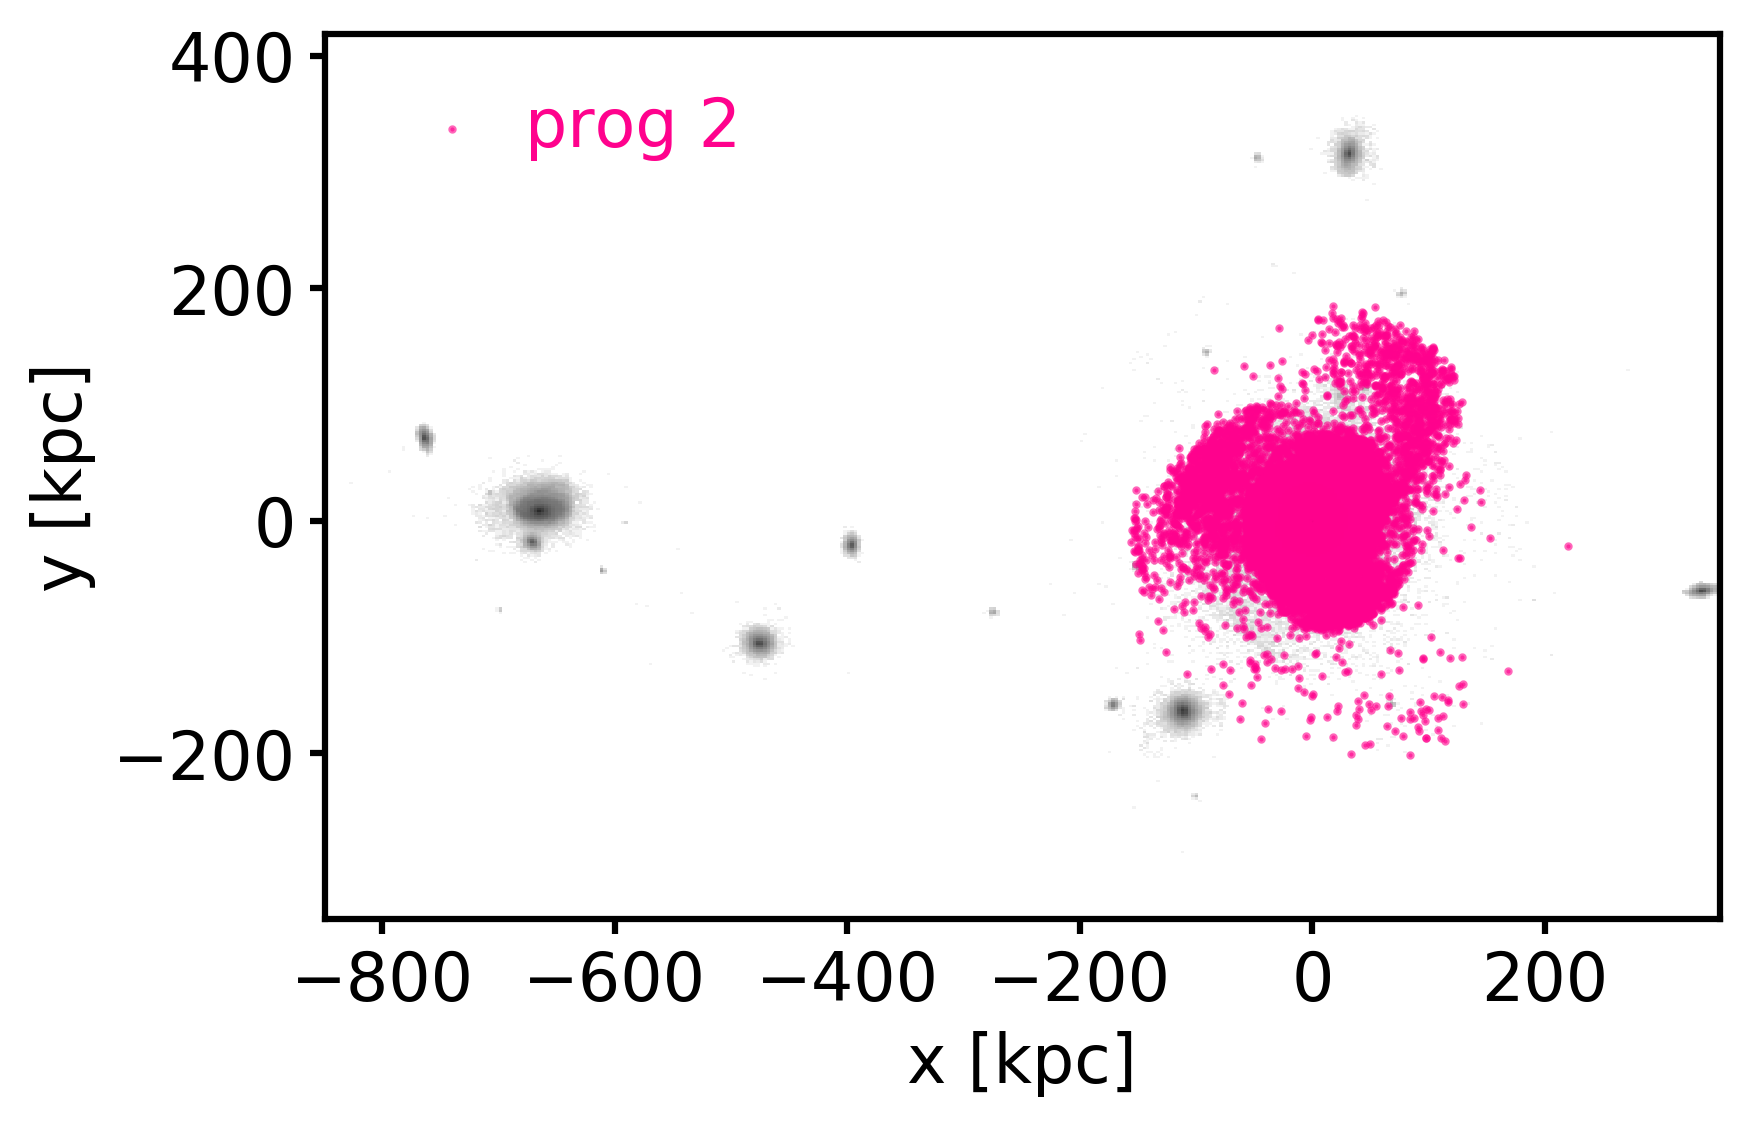
\includegraphics[width=\textwidth]{plots/Dynamics/dist/xy_dist_wodisk_GCs_prog_2_snap_127.png}
    	\label{fig:prog2_xy}
    \end{subfigure}
    ~ %add desired spacing between images, e. g. ~, \quad, \qquad, \hfill etc. 
    %(or a blank line to force the subfigure onto a new line)
    \begin{subfigure}[c]{0.48\textwidth}
        \centering
    	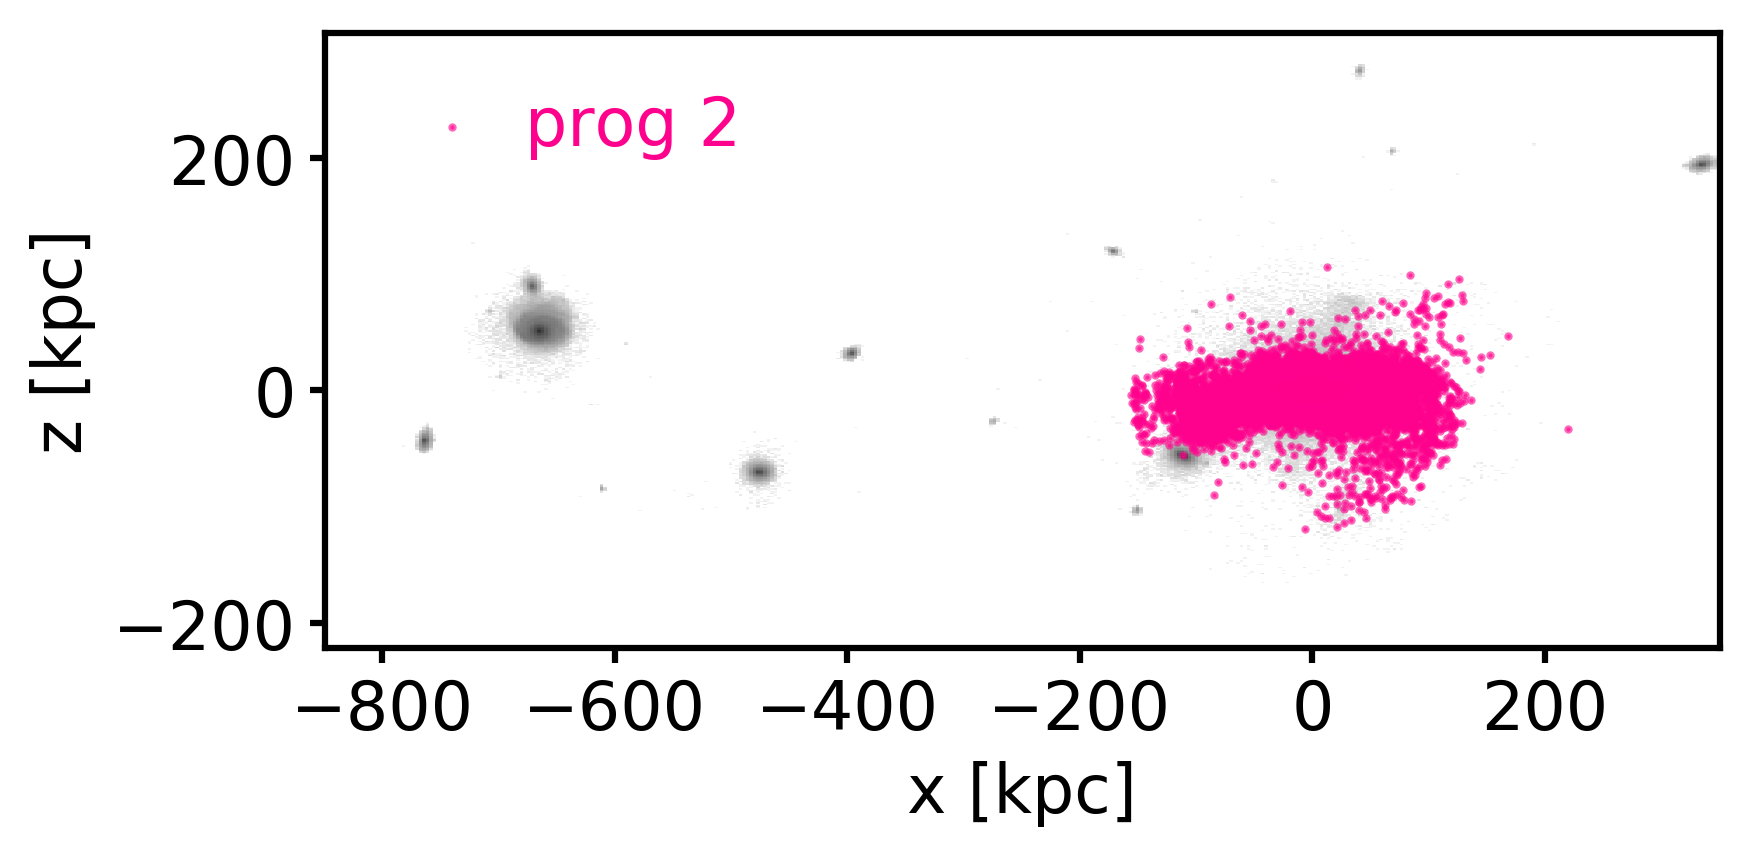
\includegraphics[width=\textwidth]{plots/Dynamics/dist/xz_dist_wodisk_GCs_prog_2_snap_127.png}
	    \label{fig:prog2_xz}
    \end{subfigure}
    
    \begin{subfigure}[c]{0.48\textwidth}
    \centering
    	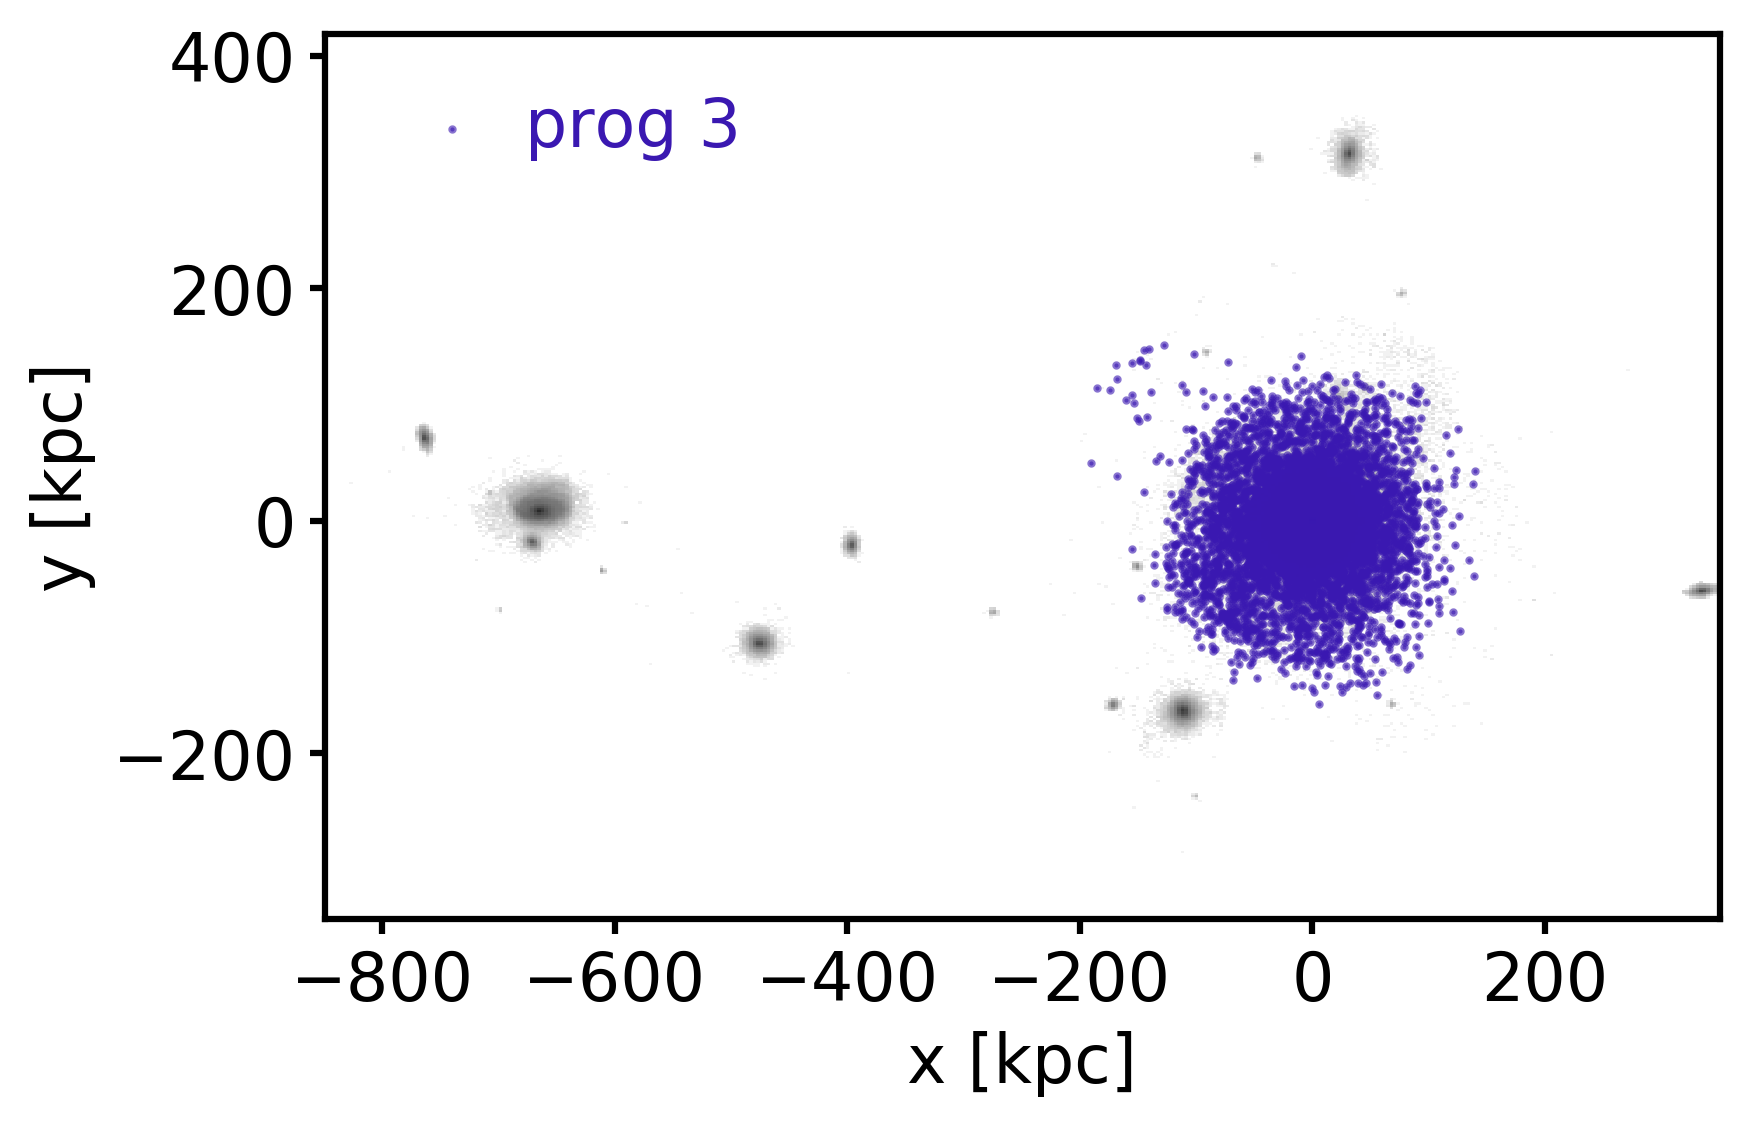
\includegraphics[width=\textwidth]{plots/Dynamics/dist/xy_dist_wodisk_GCs_prog_3_snap_127.png}
    	\label{fig:prog3_xy}
    \end{subfigure}
    ~ %add desired spacing between images, e. g. ~, \quad, \qquad, \hfill etc. 
    %(or a blank line to force the subfigure onto a new line)
    \begin{subfigure}[c]{0.48\textwidth}
        \centering
    	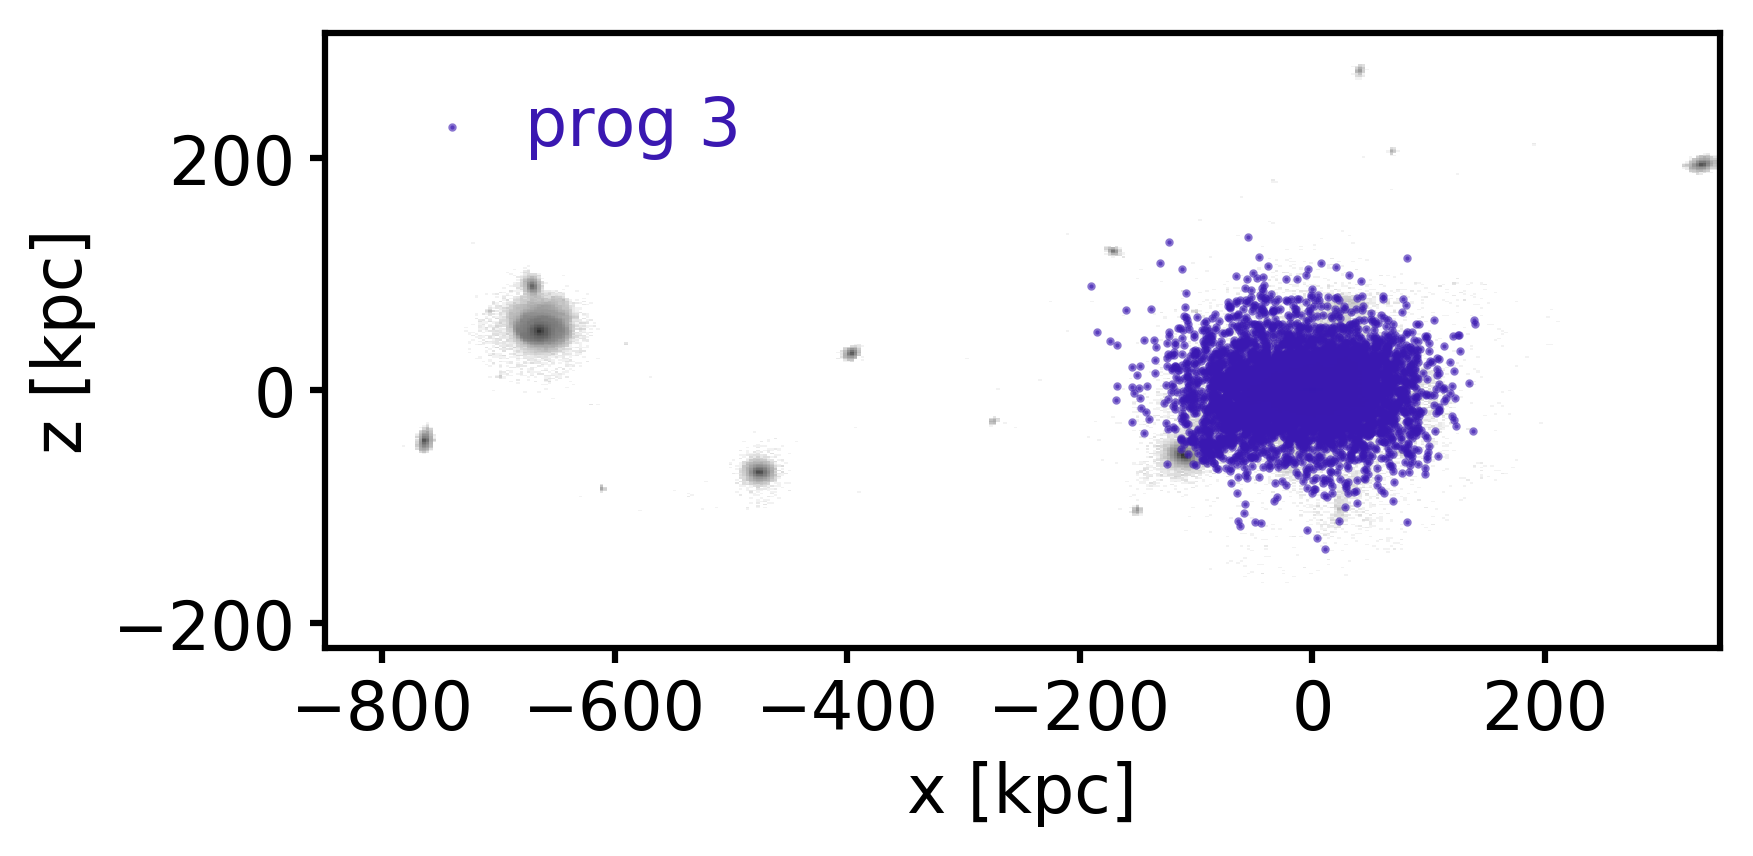
\includegraphics[width=\textwidth]{plots/Dynamics/dist/xz_dist_wodisk_GCs_prog_3_snap_127.png}
	    \label{fig:prog3_xz}
    \end{subfigure}
    
    \begin{subfigure}[c]{0.48\textwidth}
    \centering
    	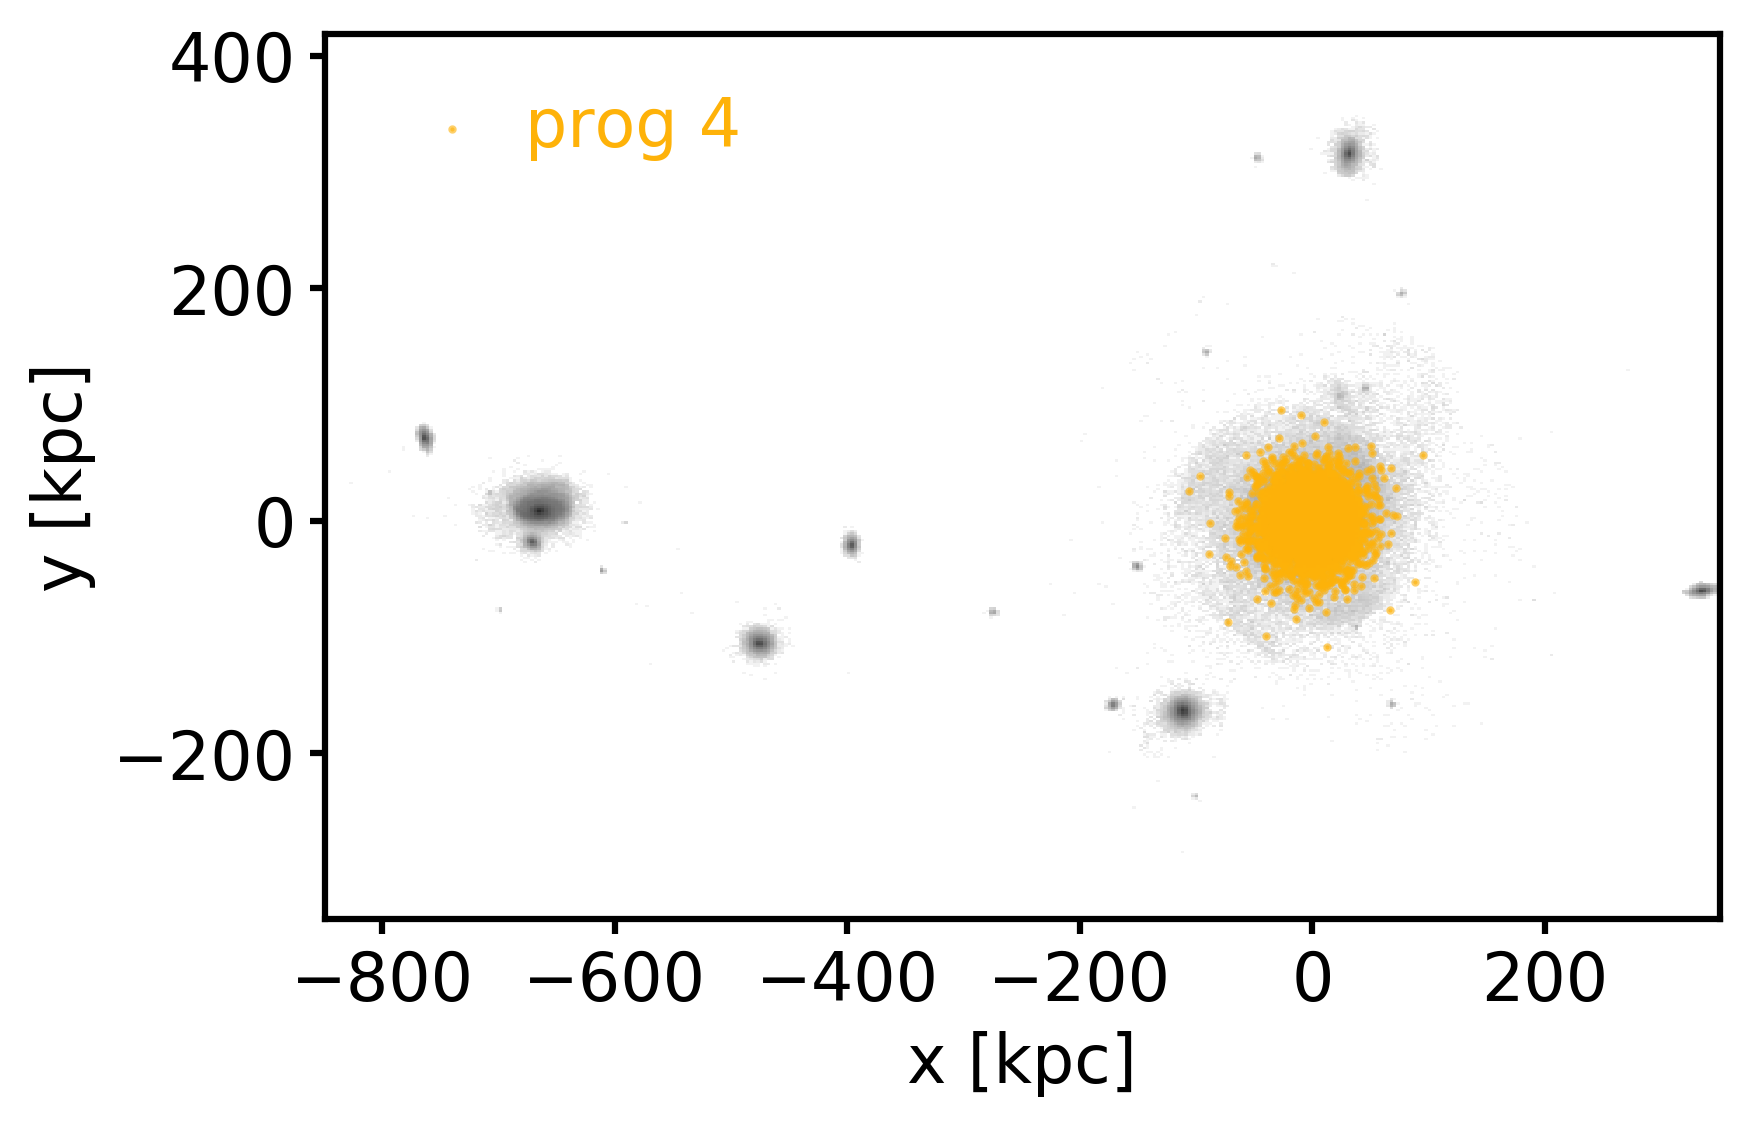
\includegraphics[width=\textwidth]{plots/Dynamics/dist/xy_dist_wodisk_GCs_prog_4_snap_127.png}
    	\label{fig:prog4_xy}
    \end{subfigure}
    ~ %add desired spacing between images, e. g. ~, \quad, \qquad, \hfill etc. 
    %(or a blank line to force the subfigure onto a new line)
    \begin{subfigure}[c]{0.48\textwidth}
        \centering
    	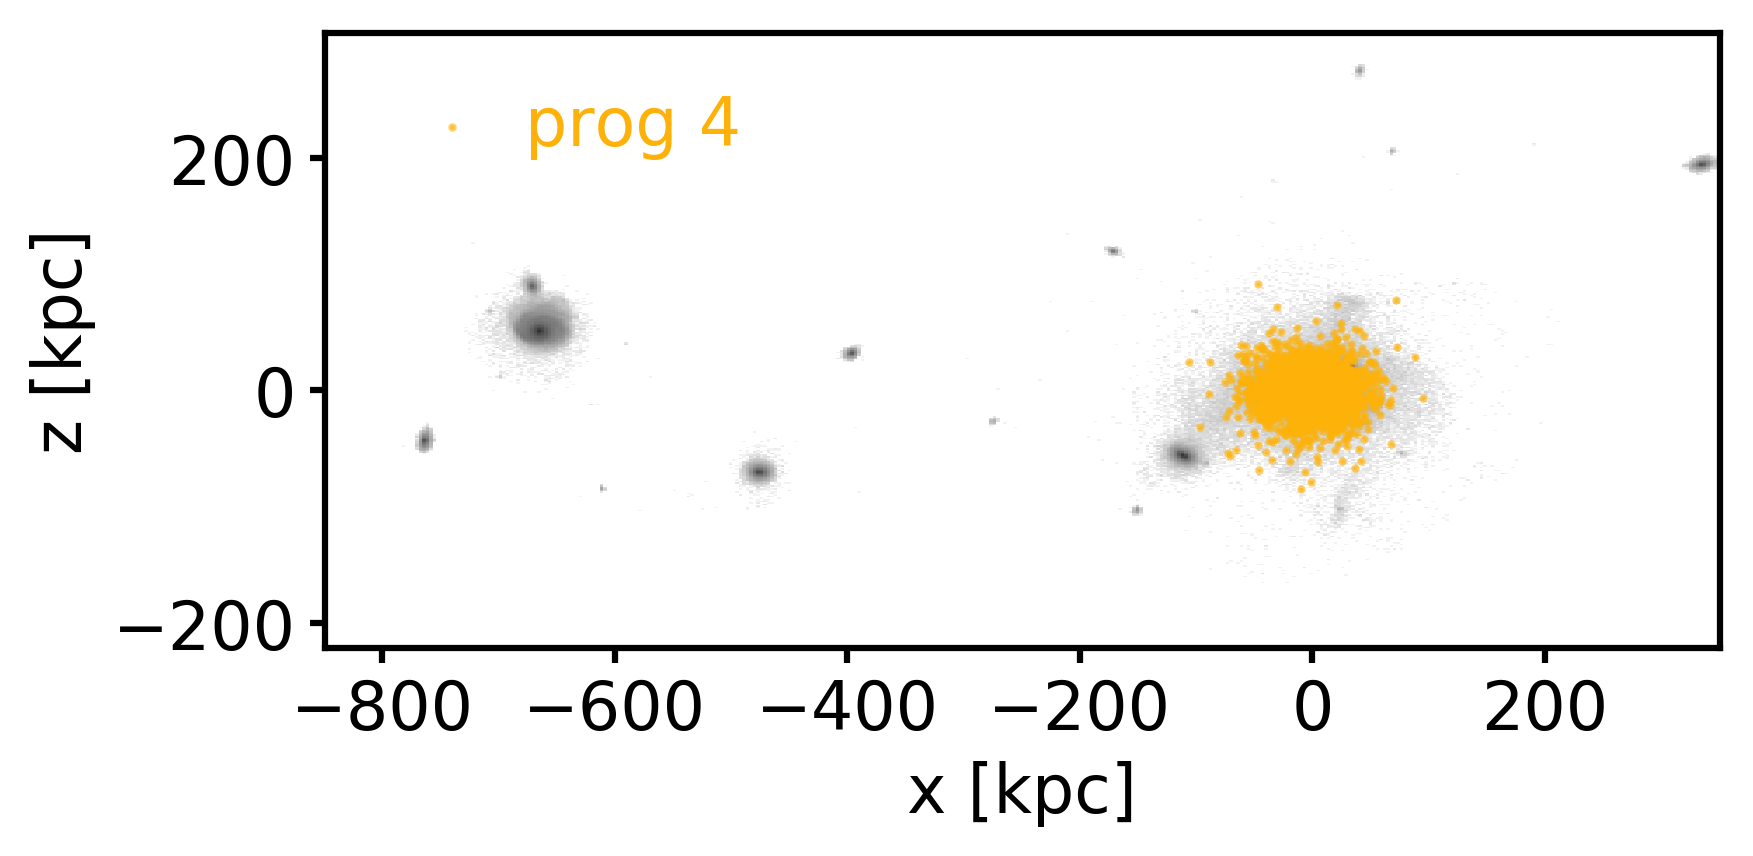
\includegraphics[width=\textwidth]{plots/Dynamics/dist/xz_dist_wodisk_GCs_prog_4_snap_127.png}
	    \label{fig:prog4_xz}
    \end{subfigure}
    \caption{Remnants of the three biggest \ac{DG} mergers which were not destroyed by the disk. The left panels show the $x-y$ distribution, the right panels the $x-z$ distribution. In grey, the main galaxy and its satellites are plotted (as in Figure \ref{fig:Stars_AU24}). \textit{Upper panels}: The remnants of the most recent merger are plotted in pink. \textit{Middle panel}: The blue points are remnants of the second biggest merger. \textit{Lower panel}: The yellow points are remnants of the third biggest merger which is the most long ago of these three. These remnants will be considered the \ac{GC} populations of each merger event.}\label{fig:progenitors_distribution}
\end{figure}
The positions of the remnants of these three merger events are shown in Figure \ref{fig:progenitors_distribution}. Prog3 and prog4 are totally dispersed in the galaxy while prog2 still shows some merging features such as broad streams, especially visible face-on. 

\subsection{Globular clusters in action space}\label{subsec:GCs_action_space}
Now, we look at the \ac{GC} distribution in action space. Our assumption is that in the "true" potential, \acp{GC} are very clumped since they should retain dynamical memory from their former \ac{DG}'s orbit and therefore their \ac{DF} should be a delta function. In Section \ref{subsubsec:GCs_actions_right_pot}, we will look at the distribution in the fitted potential at redshift 0. In Section \ref{subsubsec:GCs_actions_varying_pot}, we evaluate actions in varying potentials to test our assumption of \acp{GC} being most clumped in action space in the "true" potential. 

\subsubsection{Best fit potential}\label{subsubsec:GCs_actions_right_pot}

\begin{figure}[htbp]
\captionsetup{format=plain}
    \centering
    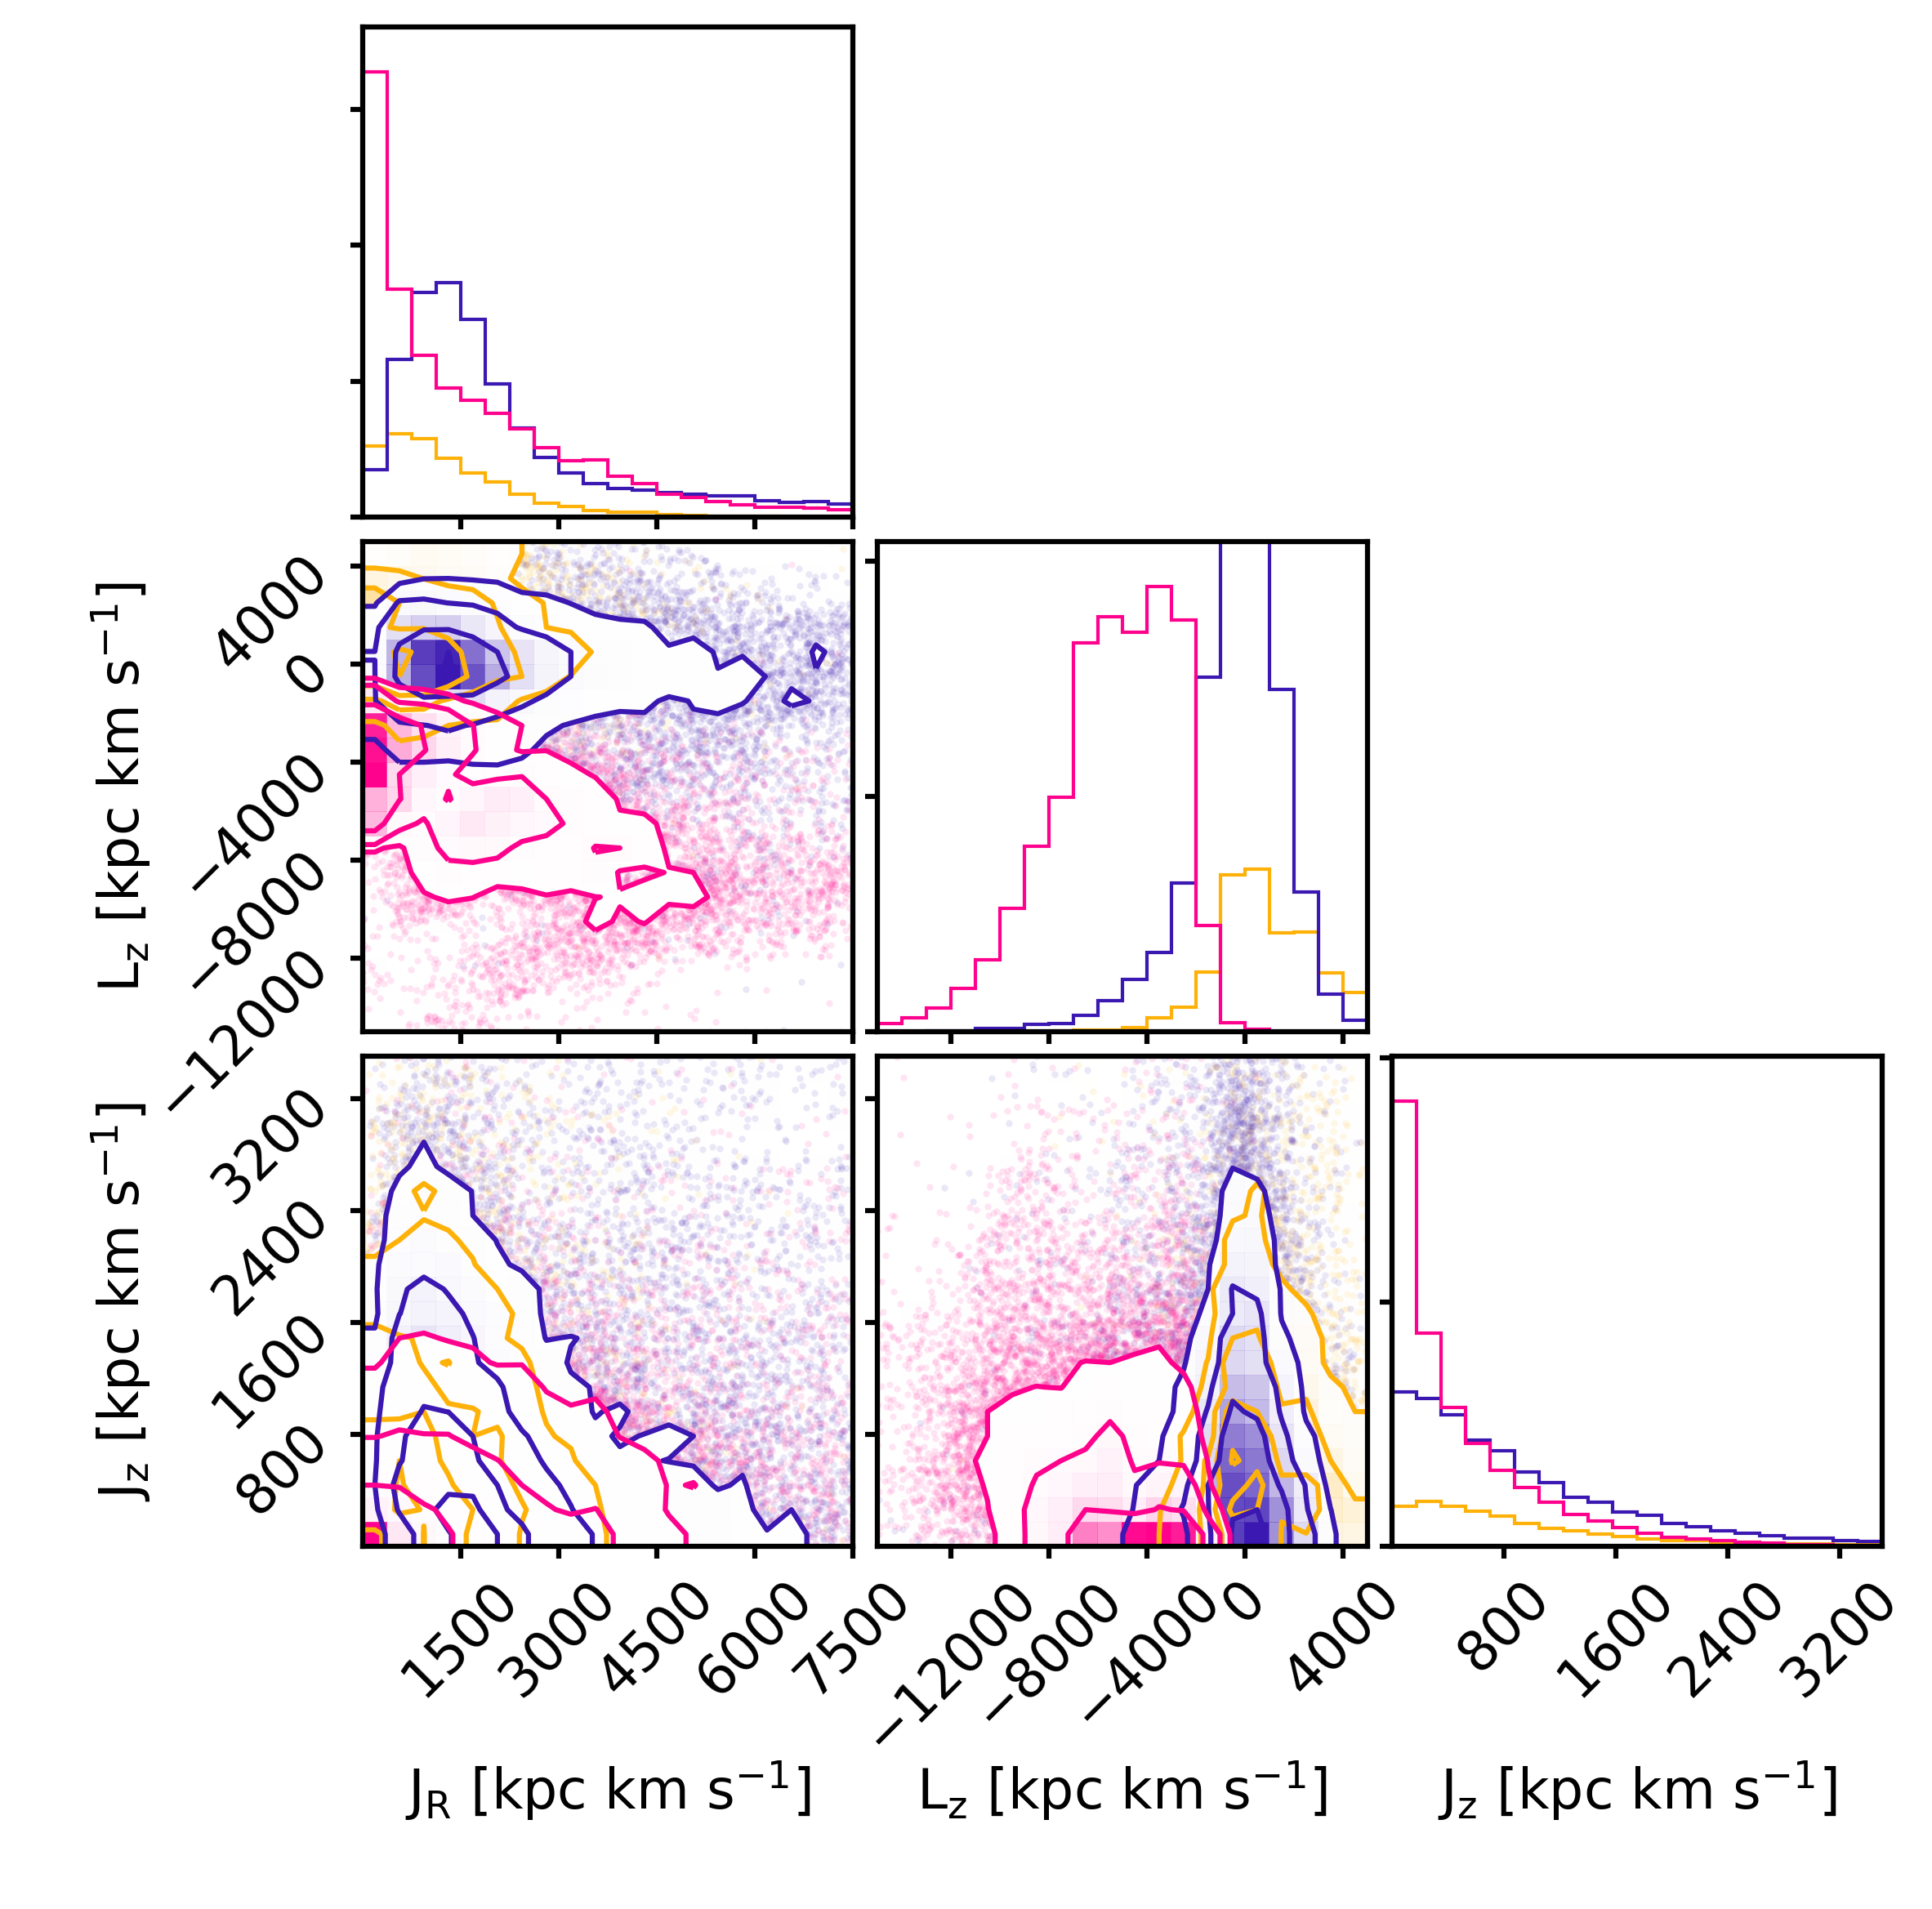
\includegraphics[width=1.0\textwidth]{plots/Dynamics/prog234_GCwodisk_actions_snap_127.png}
    \caption{Selected \acp{GC} from three different \acp{DG} in action space. The diagonal elements show histograms of each action and the other panels show 2D histograms of each action pair. In pink/blue/yellow, we see the action distribution of the remnants of prog2/prog3/prog4. Prog2 and prog3 have more particles than prog4 and therefore dominate the 1D histograms in the diagonal elements. In the correlation panels, we can clearly distinguish prog2 in $L_z$ and $J_R$ while prog3 and prog4 distribute around the same means. The distribution of prog2 is broad in $L_z$ and more narrow in $J_R - J_z$. prog2 is corotating with the disk but with a higher angular momentum than the disk has (\(\overline{L_z} = \SI{-2235}{kpc.km.s^{-1}}\)). prog3 and prog4 have a mean angular momentum of 0 and mean higher radial action than prog2. Their motion seems to be independent of the disk. All groups have rather broad distributions in the actions.}
    \label{fig:act_all_merg_best_pot}
\end{figure}
We calculate the actions of the remnants of each progenitor in the best fit potential from the coordinates ($R, \phi, z, v_r, v_\phi, v_z$) at \textit{z=0} and plot them in Figure \ref{fig:act_all_merg_best_pot}. The most recent remnant, prog2, is most distinguishable in $L_z$. It is corotating with the disk but with higher angular momentum. Prog3 and prog4 are not rotating. In the vertical action, the three remnant groups are not distinguishable and have means close to \SI{0}{kpc.km.s^{-1}}. In $J_R$, the groups are again distinguishable since prog2 has a mean $J_R = \SI{0}{kpc.km.s^{-1}}$ while the older remnants have a higher radial oscillation. Prog2 seems to have merged in the disk plane while prog3 and prog4 have dispersed more spherically. We can see this spatial distribution in Figure \ref{fig:progenitors_distribution} where we also notice that prog2 has not fully merged yet.
\\The idea of this method is that in the right potential, these groups minimize their spread in action space. Prog4 is the most compact group, while especially prog3 is very dispersed. None of the distributions looks like a $\delta$-function. To quantify the compactness, we measure the standard deviation of each action. In the next Section, we compare the standard deviations of the radial and vertical actions of each group in different potentials to see, if we minimize them in the "true" potential.

\subsubsection{Varying potentials}\label{subsubsec:GCs_actions_varying_pot}
The \acp{GC} are at distances where the potential is dominated by the \ac{DM} halo (see Figure \ref{fig:circ_vel_fit}). Variations in that component should have the biggest impact on their action space distributions. Therefore, we vary the \ac{DM} halo by keeping all best fit potential parameters constant and only vary the scale length $a_\mathrm{NFW}$. For the three groups in these potentials, we calculate the actions in the $z=0$ snapshot.
\begin{figure}[!ht]
\captionsetup{format=plain}
   \subfloat{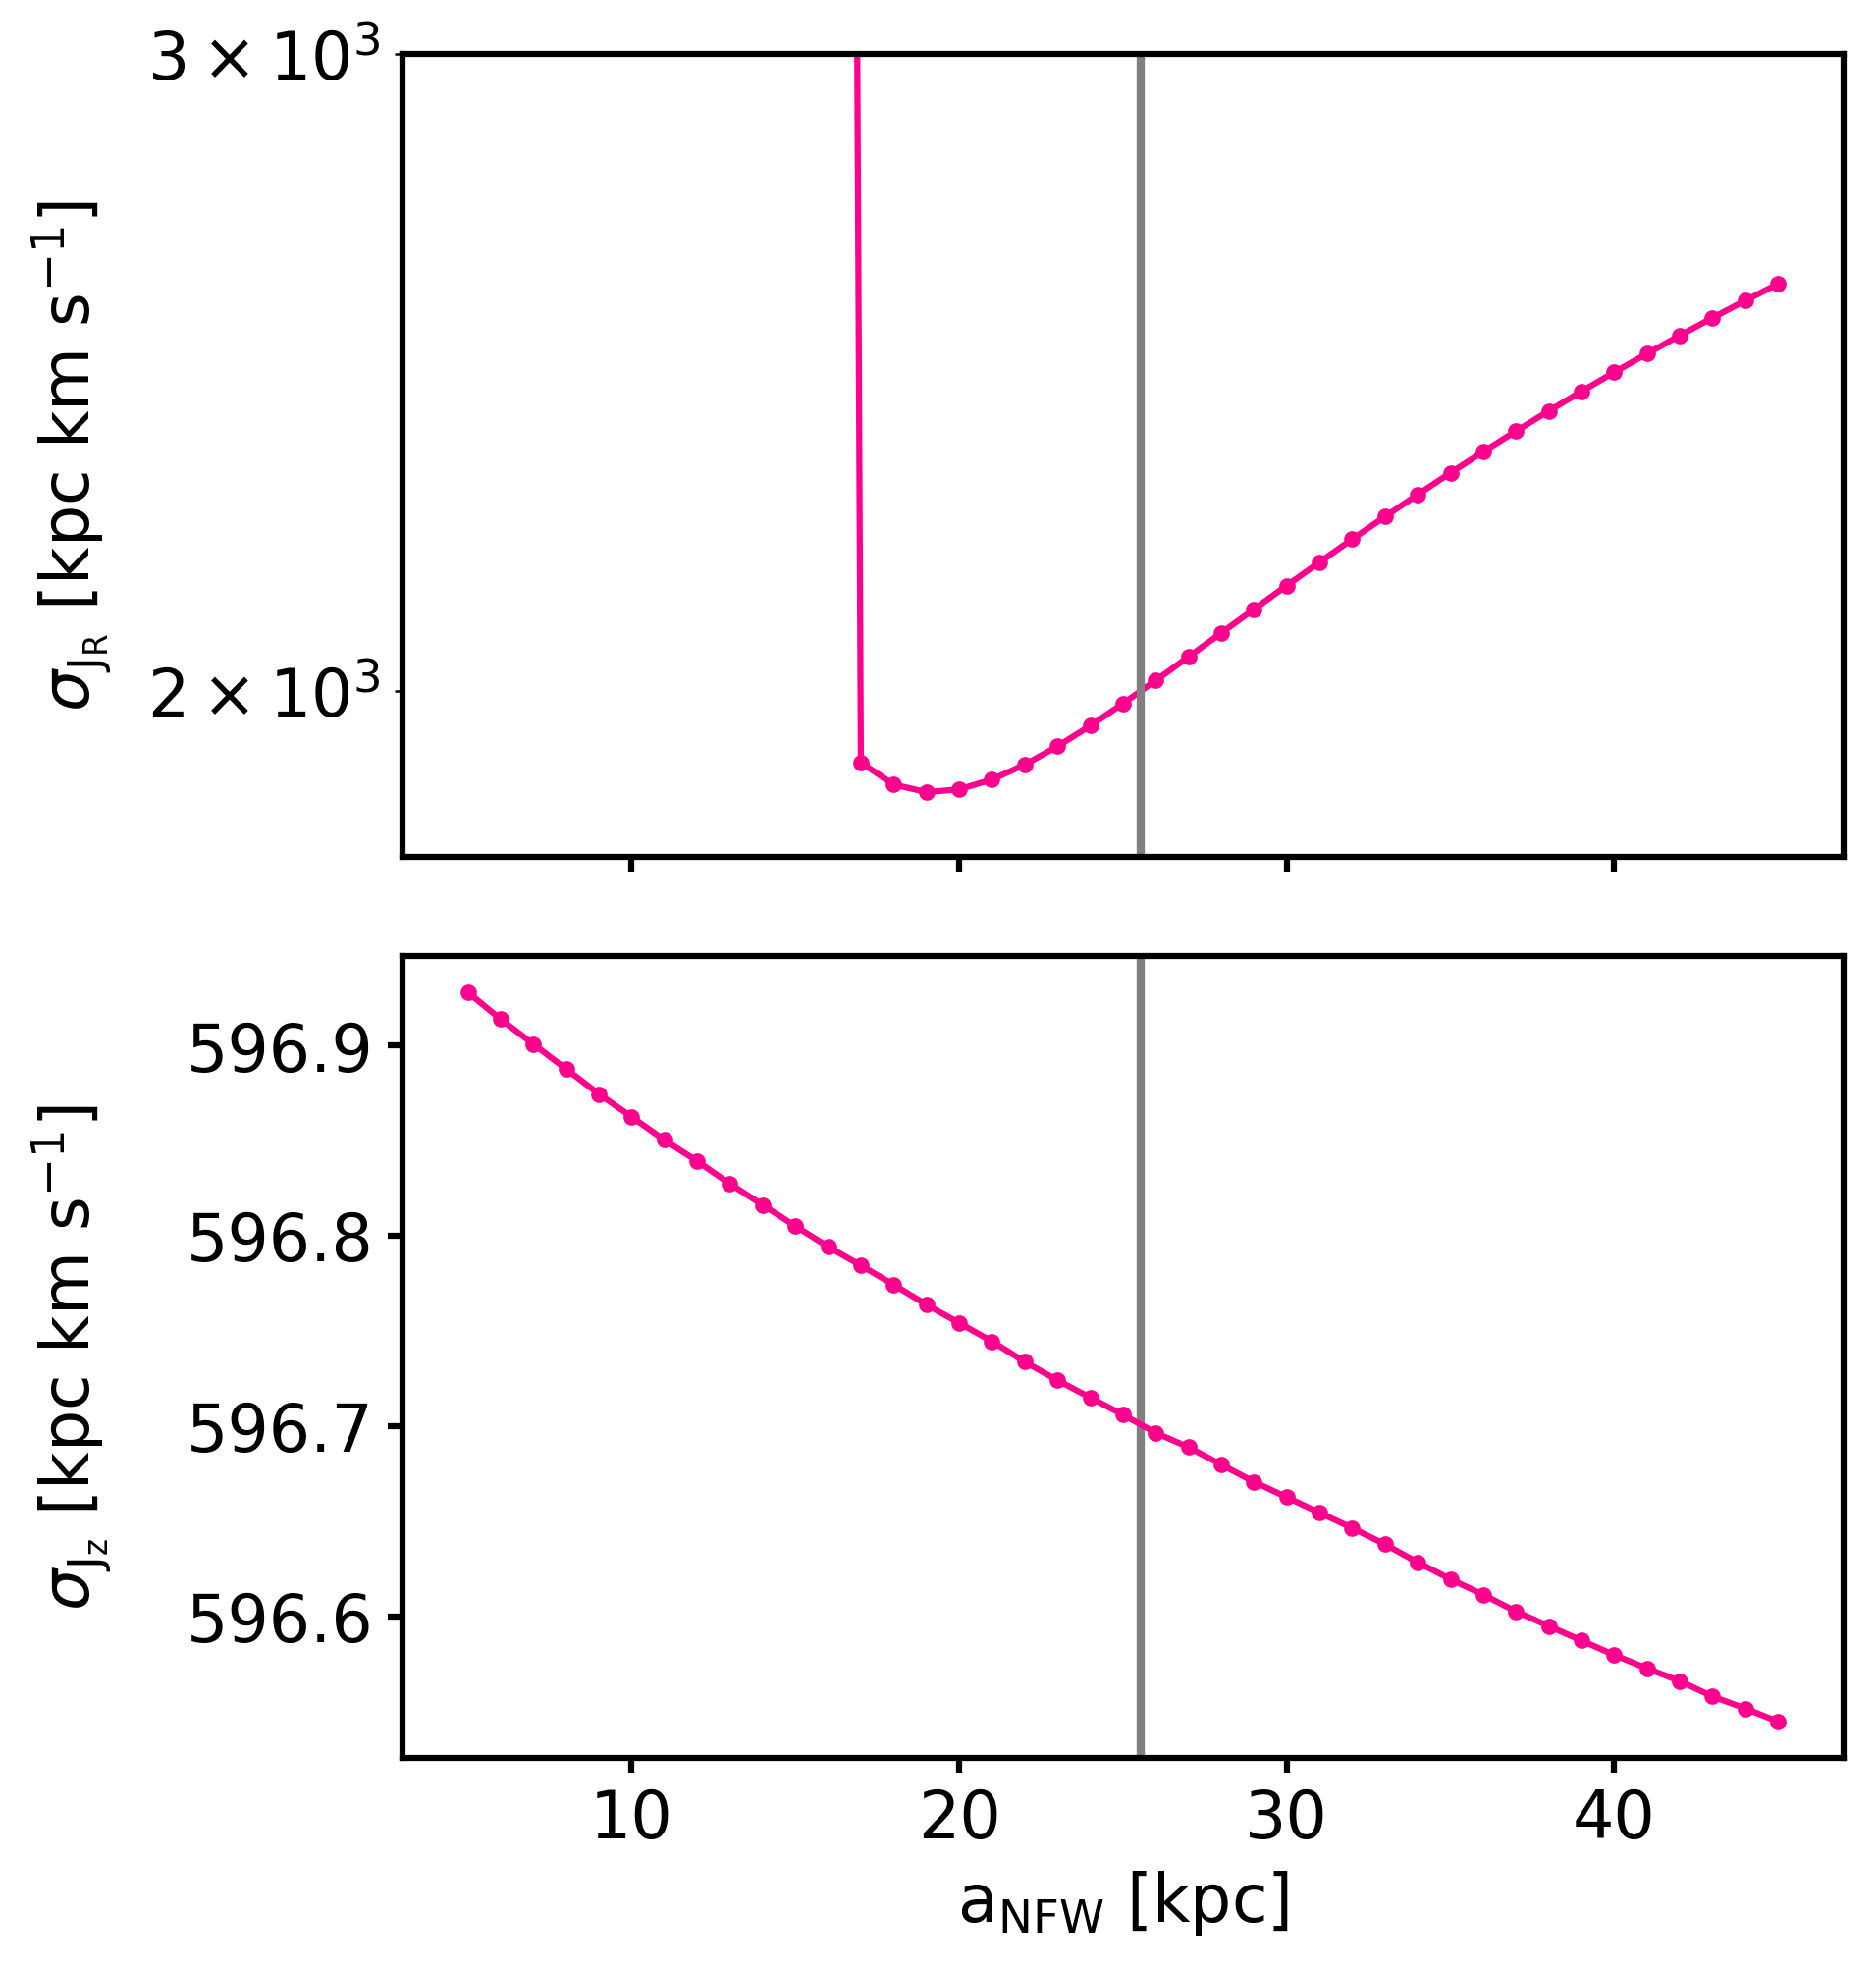
\includegraphics[width=0.48\textwidth]{plots/Dynamics/prog2/a_NFW_diagnostic_plot_std_wodiskchange_prog2_all.png}}\hfill%
   \subfloat{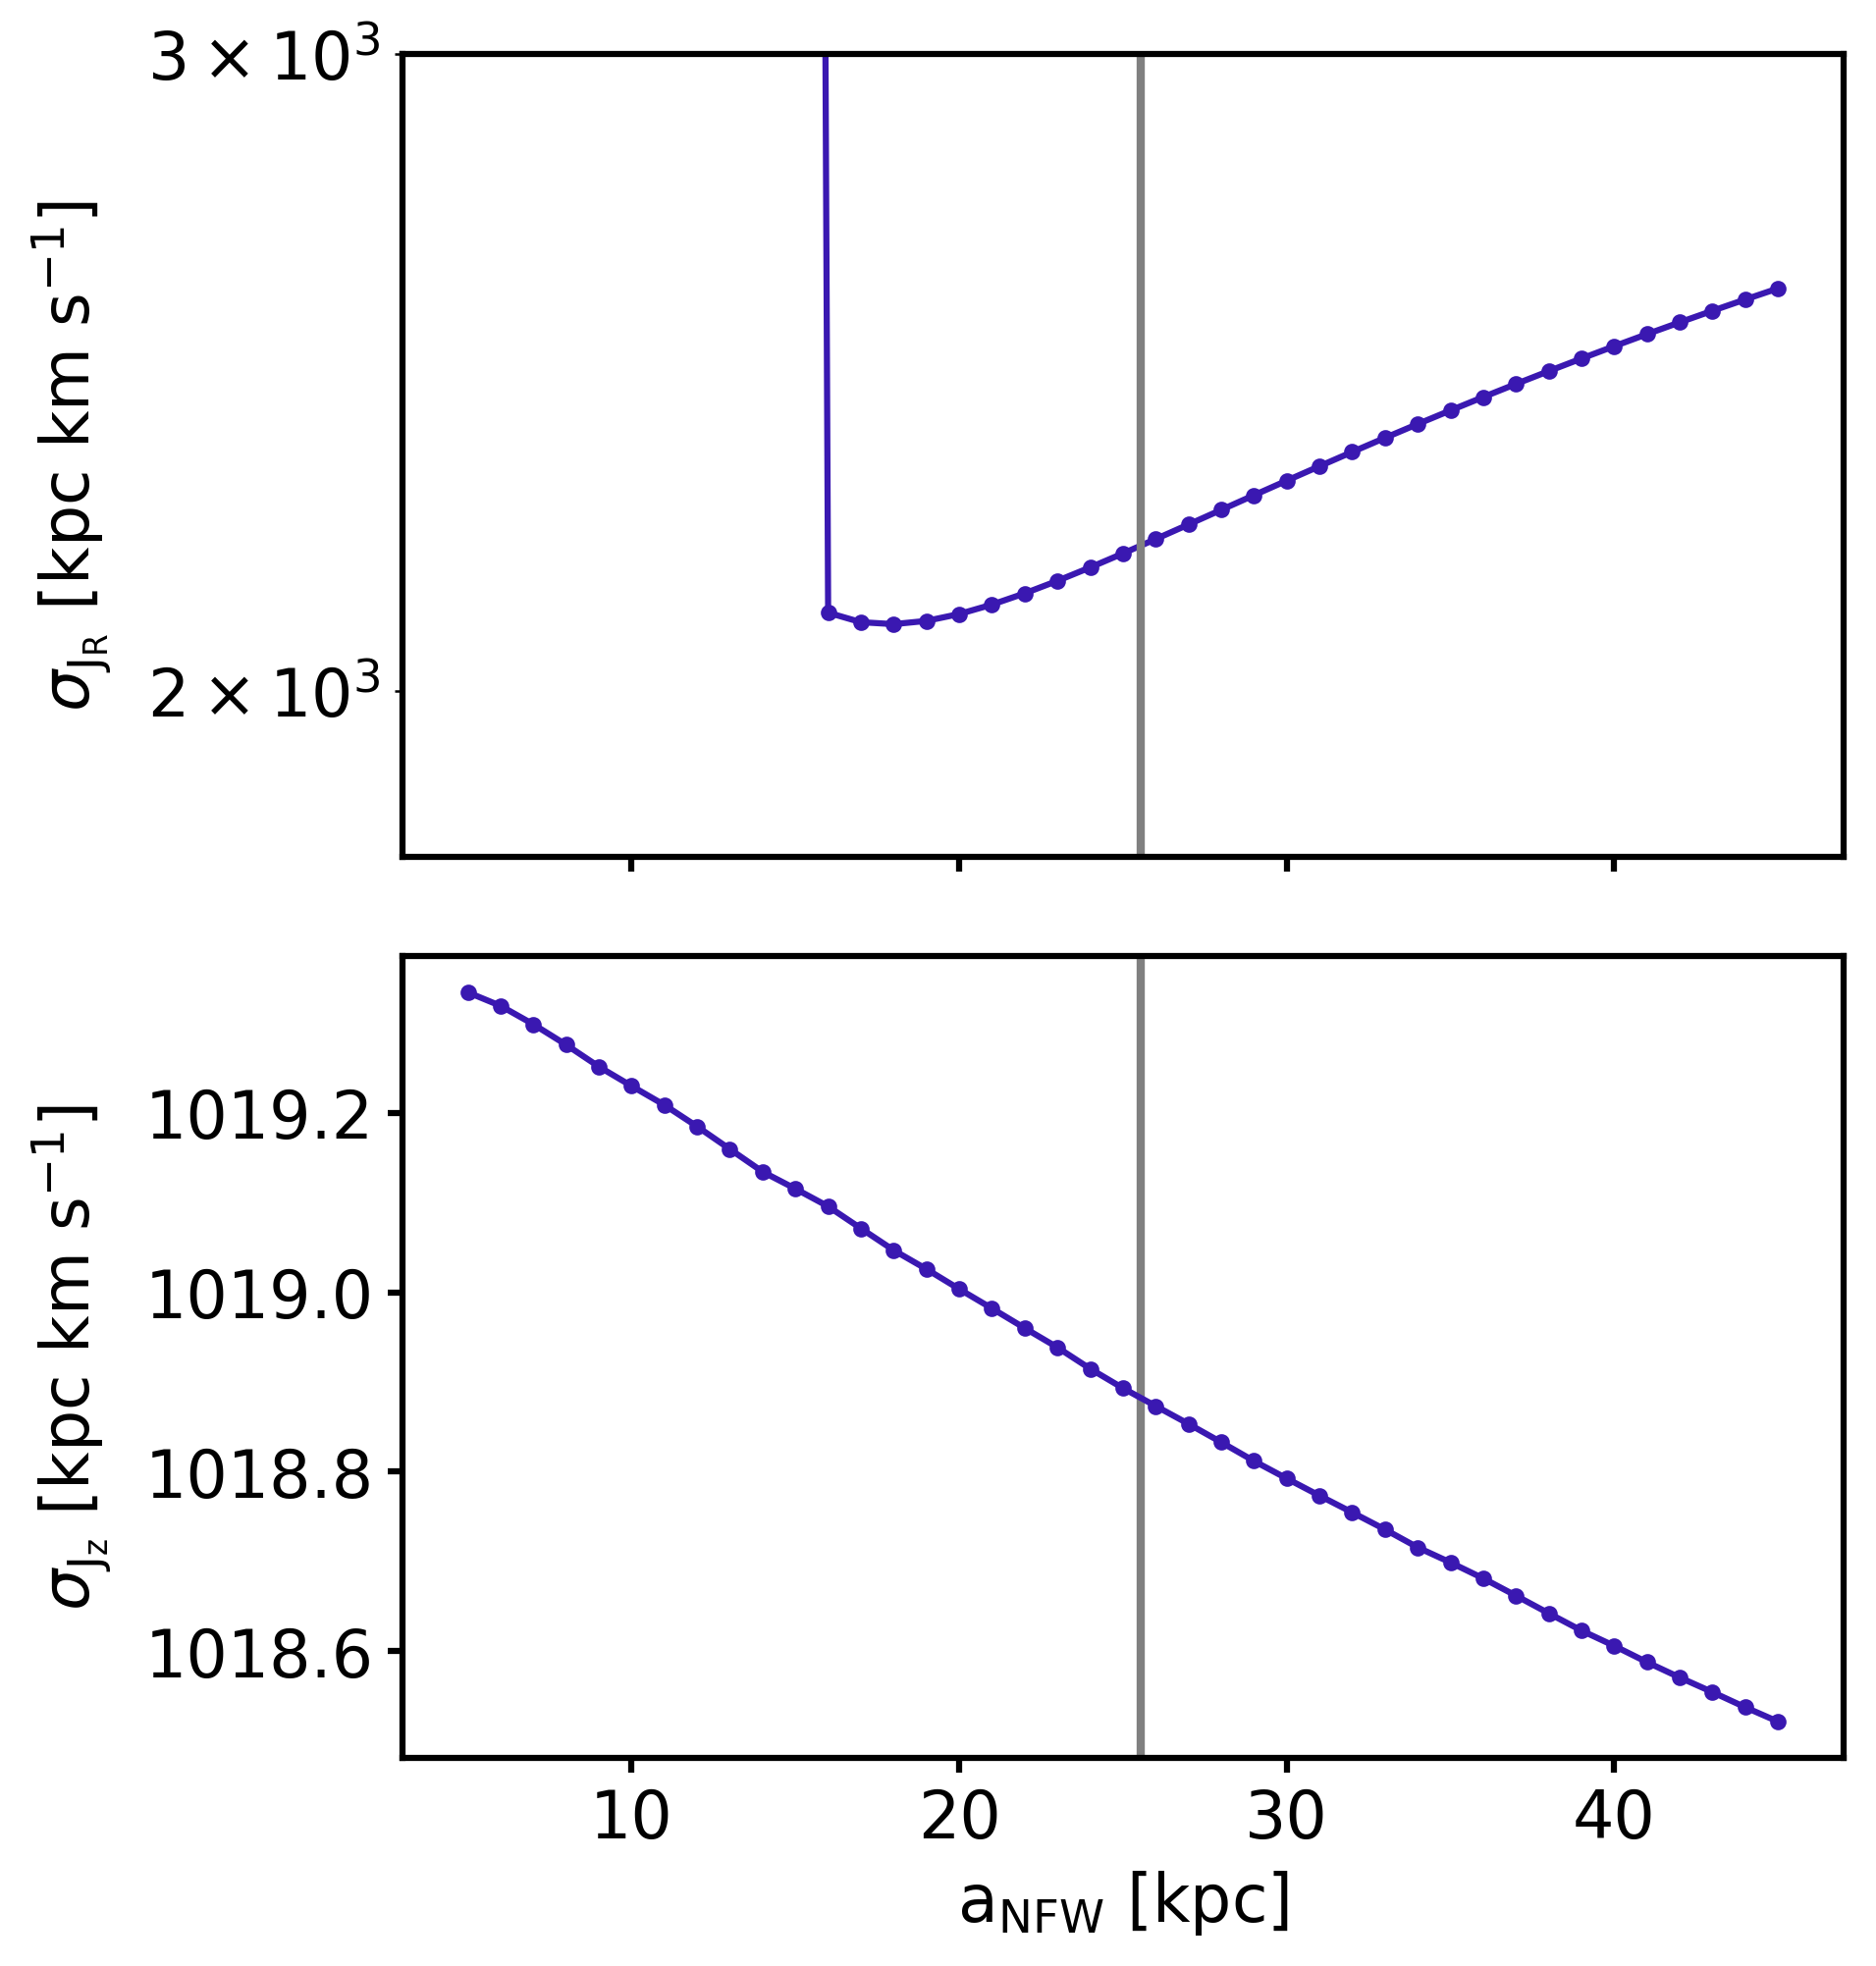
\includegraphics[width=0.48\textwidth]{plots/Dynamics/prog3/a_NFW_diagnostic_plot_std_wodiskchange_prog3_all.png}}\vspace*{0.5cm}\par
   \subfloat{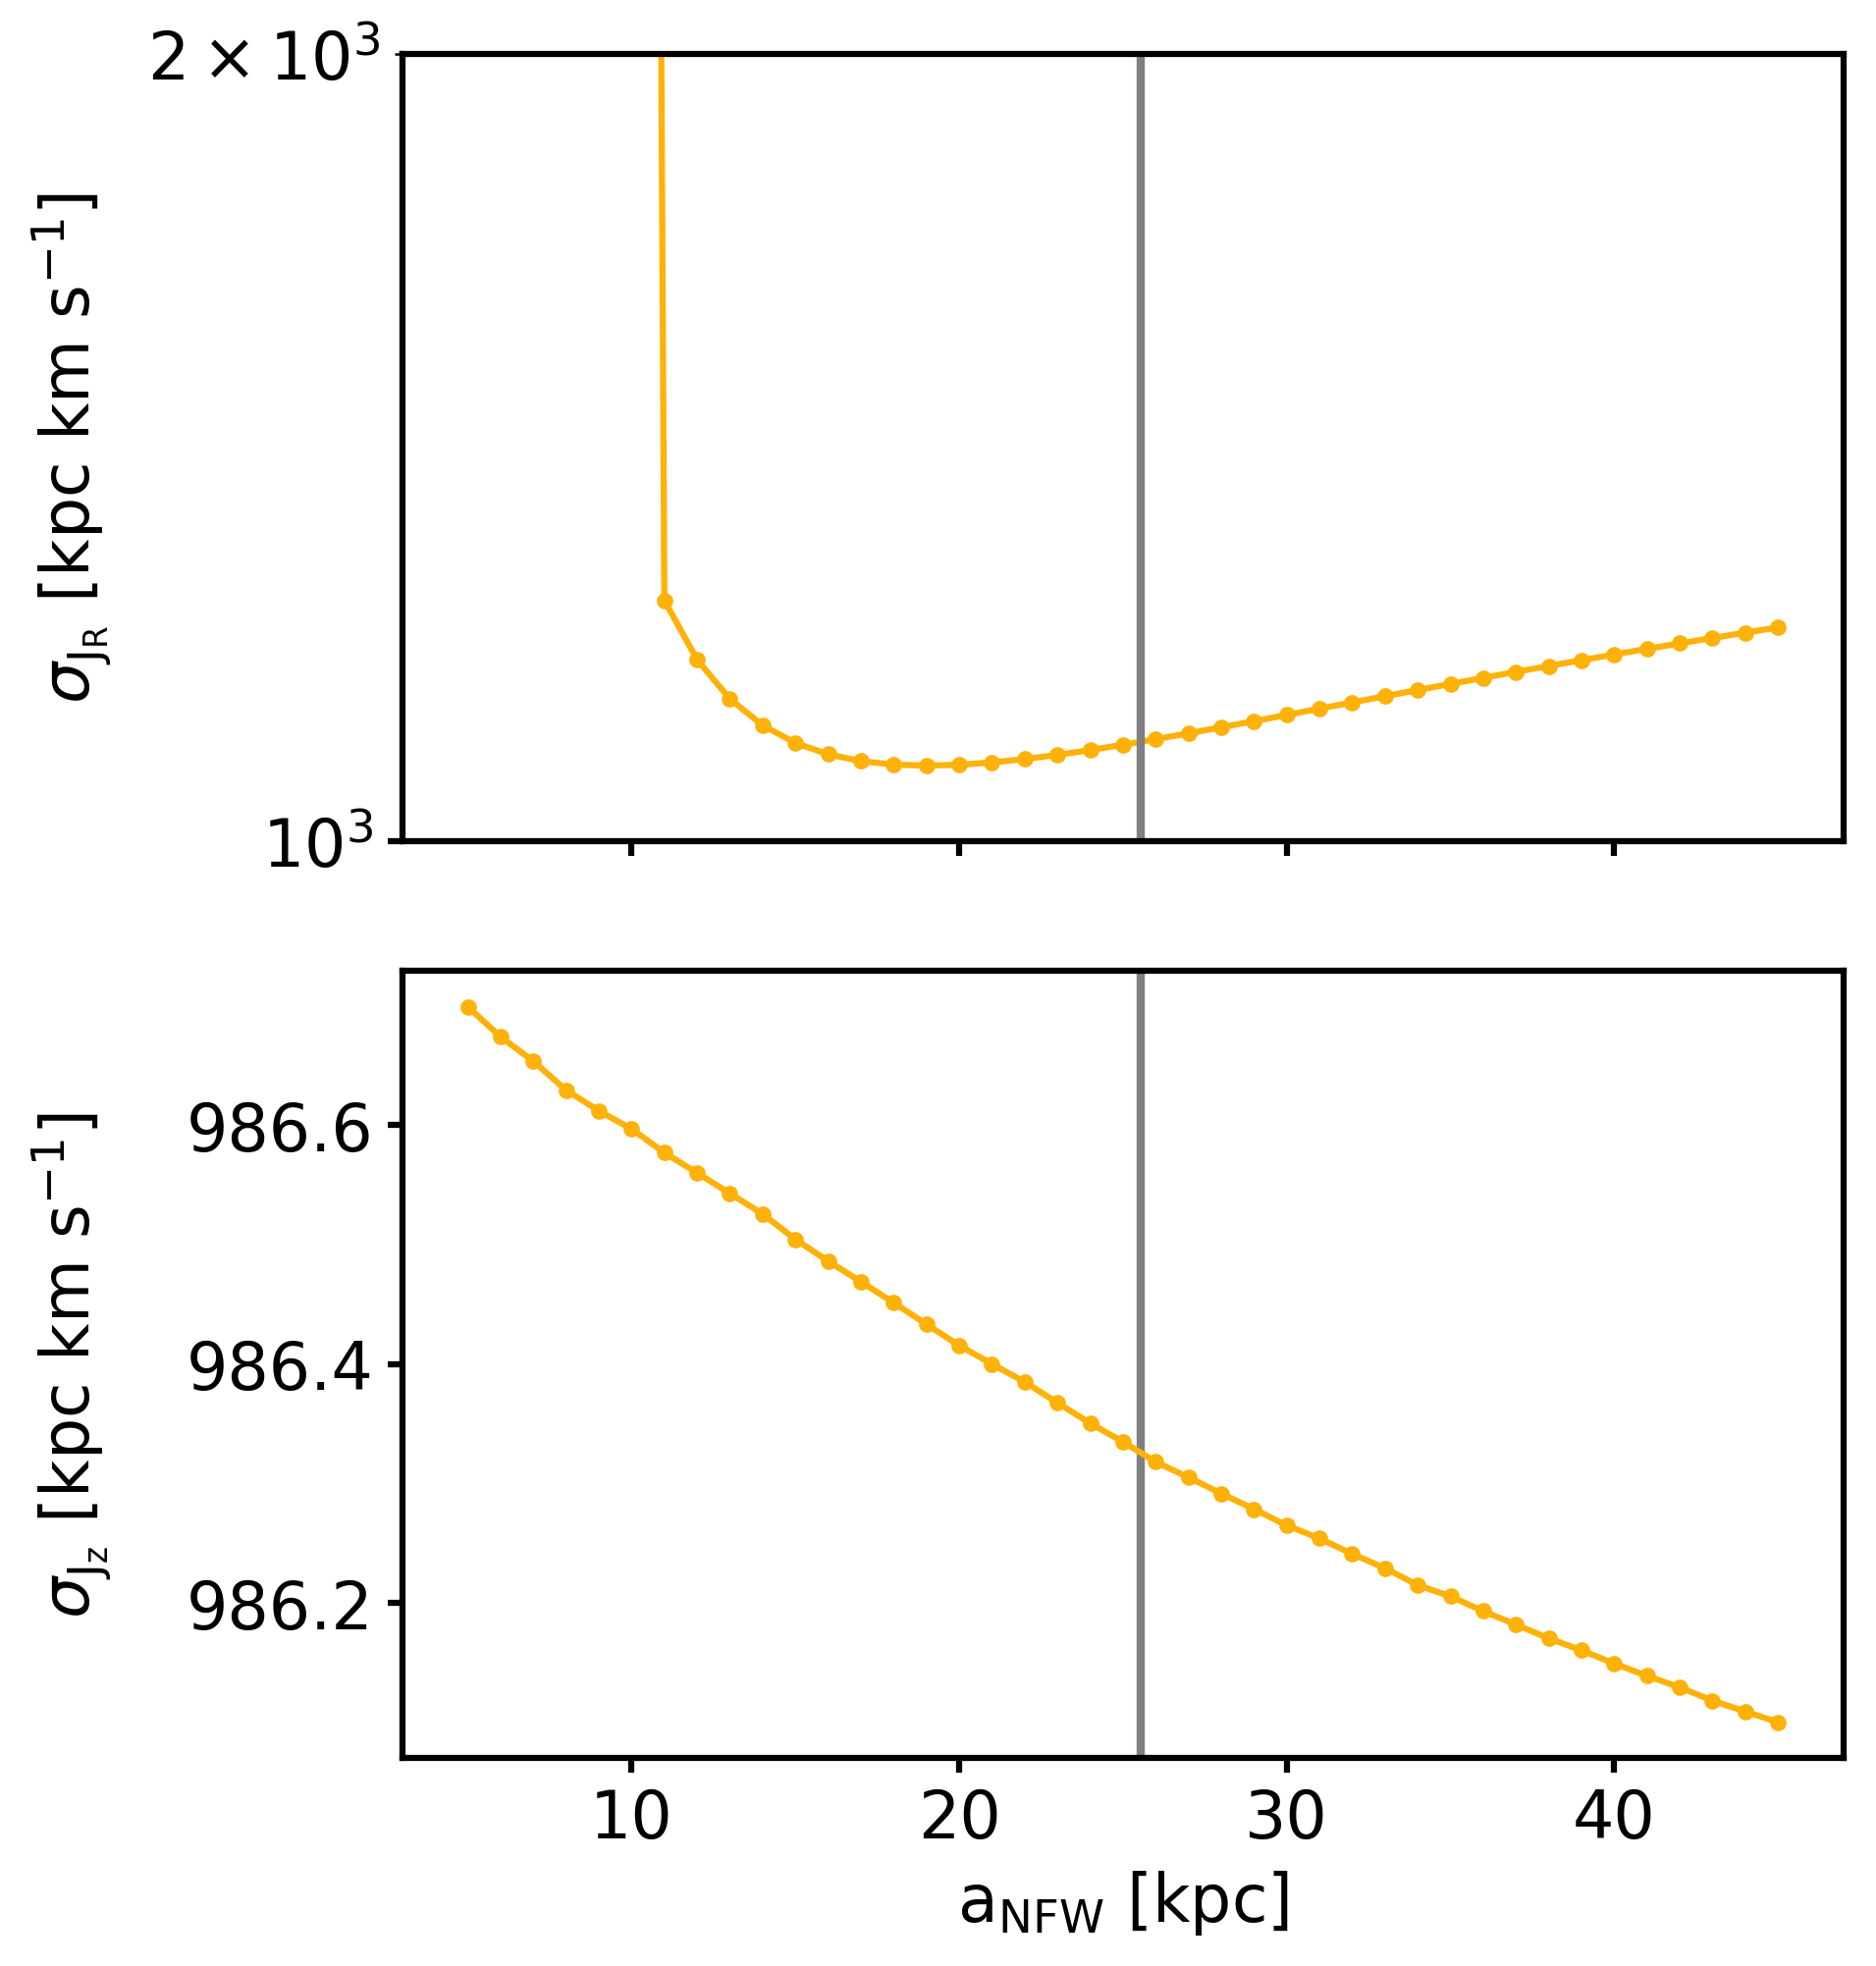
\includegraphics[width=0.48\textwidth]{plots/Dynamics/prog4/a_NFW_diagnostic_plot_std_wodiskchange_prog4_all.png}}\hfill%
   \parbox[b][.3\textheight]{.48\textwidth}%
     {\vskip-\abovecaptionskip\RawCaption{\caption{Standard deviations of the radial and vertical actions of all three mergers (prog2-pink / prog3-blue / prog4-yellow) in potentials with varying scale length of the \ac{DM} halo and all other parameters kept on their best fit value. We would expect the standard deviation to be mimized at the best fit potential which is indicated with the vertical grey line. We see that the radial action would prefer a lower scale length (at \SI{17}{kpc}) while two of the three vertical actions would prefer higher scale lengths. The differences in $\sigma_{J_z}$ are much smaller than the one in $\sigma_{J_R}$.}\vfill\label{fig:a_NFW_diagnostic_plots}}}
\end{figure}
In Figure \ref{fig:a_NFW_diagnostic_plots}, we see how the standard deviations of the radial and vertical actions evolve in the different potentials. For all three \acp{GC} groups we see that in the radial action they would prefer a smaller scale length than the true value of the halo potential. The changes in vertical action are very small but two of three groups would prefer a larger scale length than the true one. 
\\\\This leads us to the conclusion that in the "true" potential, accreted \acp{GC} of one \ac{DG} are not on similar orbits but have a \ac{DF} that is more complex. We cannot constrain an analytic axisymmetric gravitational potential by only minimizing the spread of these \acp{GC} in action space.

\subsection{Time evolution of actions}\label{subsec:time_evo_actions}
We evaluate the time evolution of the orbits of the accreted \acp{GC} to see if there was a point - probably shortly after their mergers - where the \acp{GC} were more clumped in action space and the \ac{DF} could have been a $\delta$-function. If that would be true, we could at least determine the potential of galaxies which are in a state shortly after a minor merger. We calculate the actions of the selected particles in the best fit potential in each snapshot.  

\subsubsection{Best fit potential}\label{subsubsec:GCs_action_time_right_pot}
With the method described in Section \ref{subsec:best_fit_pot} we fit an analytic axisymmetric potential to each snapshot individually and interpolate the parameters for a smooth potential evolution (see Figure \ref{fig:pot_val_evol}). We trace back the \acp{GC} we considered as merged and calculate their actions in each snapshot for both after and before the merger. 
\begin{figure}[htbp]
\captionsetup{format=plain}
    \centering
	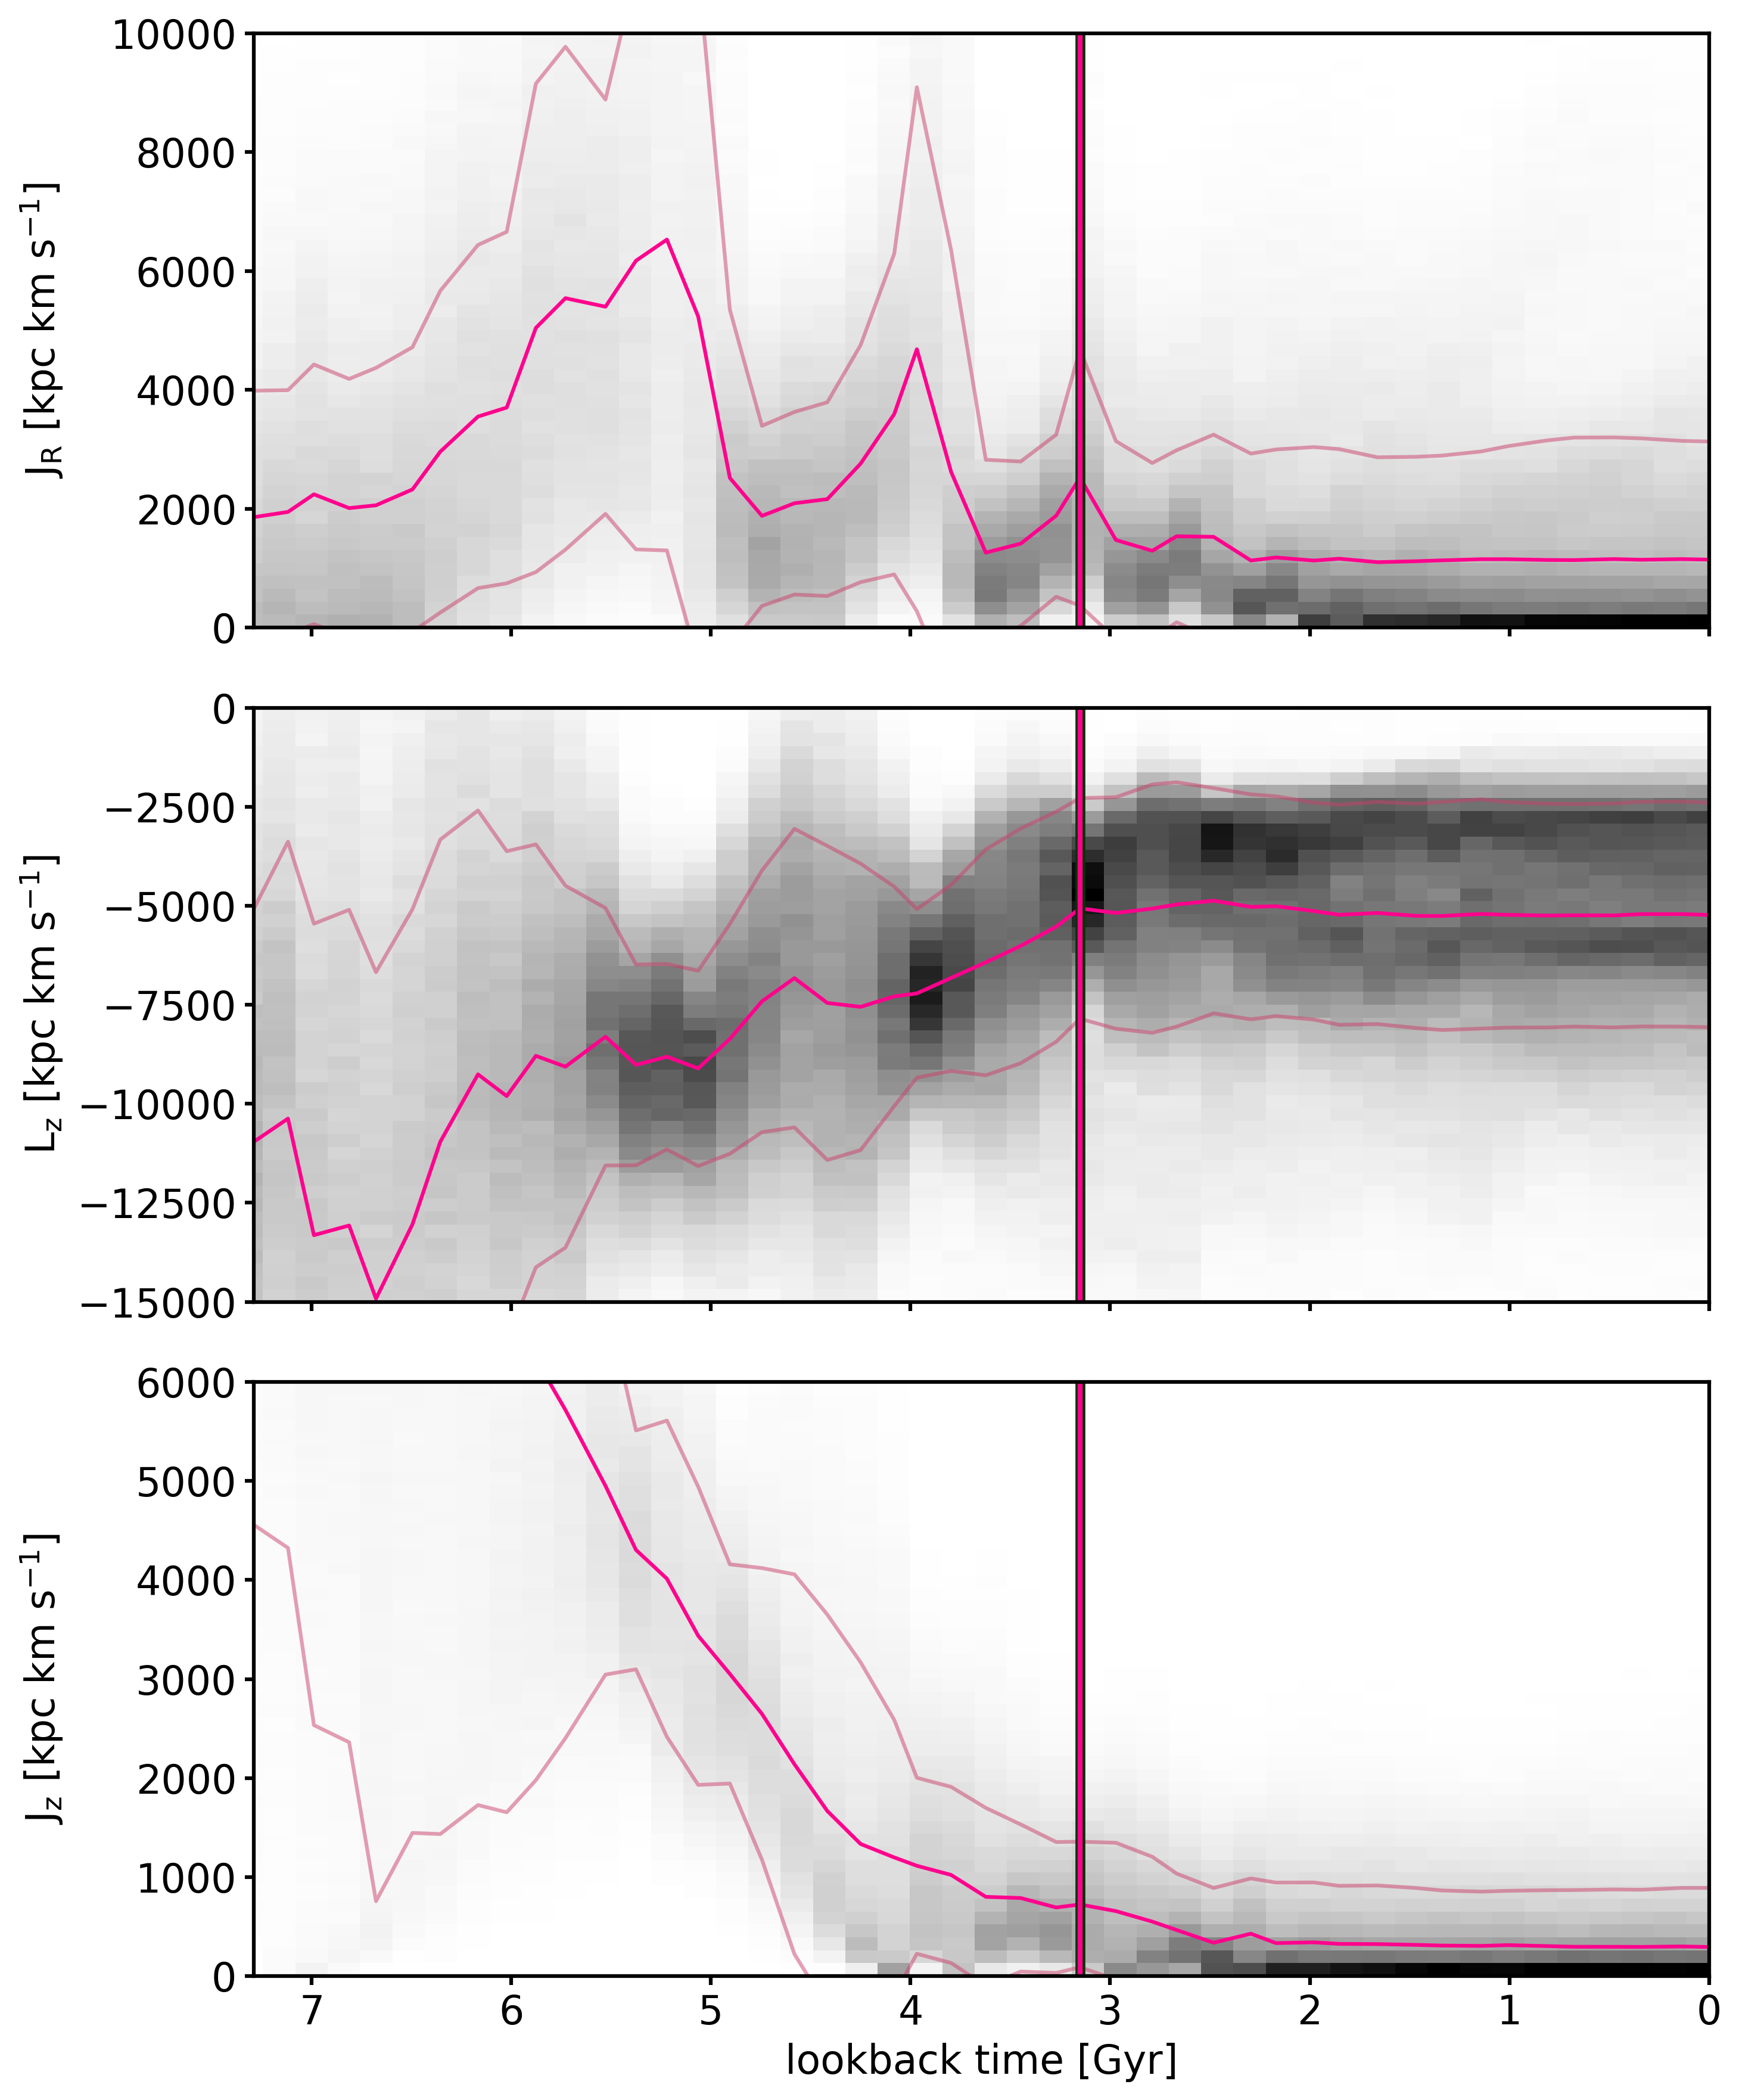
\includegraphics[width=\textwidth]{plots/Dynamics/prog2/action_time_evolution_wodisk_hist_mean.png}

	\caption{Evolution of actions of prog2 \acp{GC} over time. The pink vertical line indicates the time of the merger. The other pink lines follow the median (bright pink) and the standard deviation (light pink). \textit{Upper panel}: Radial action. \textit{Middle panel}: Angular momentum. \textit{Lower panel}: Vertical action. Before the merger, the vertical actions were much higher and all three actions had higher standard deviations. This indicates that their motions were not yet governed by our main galaxy's potential. With the merger, they have settled and all of them have a constant mean and standard deviation since $<1$ Gyr after the merger.}\label{fig:actions_time_evolution_prog2}
\end{figure}

\begin{figure}
\captionsetup{format=plain}
\centering
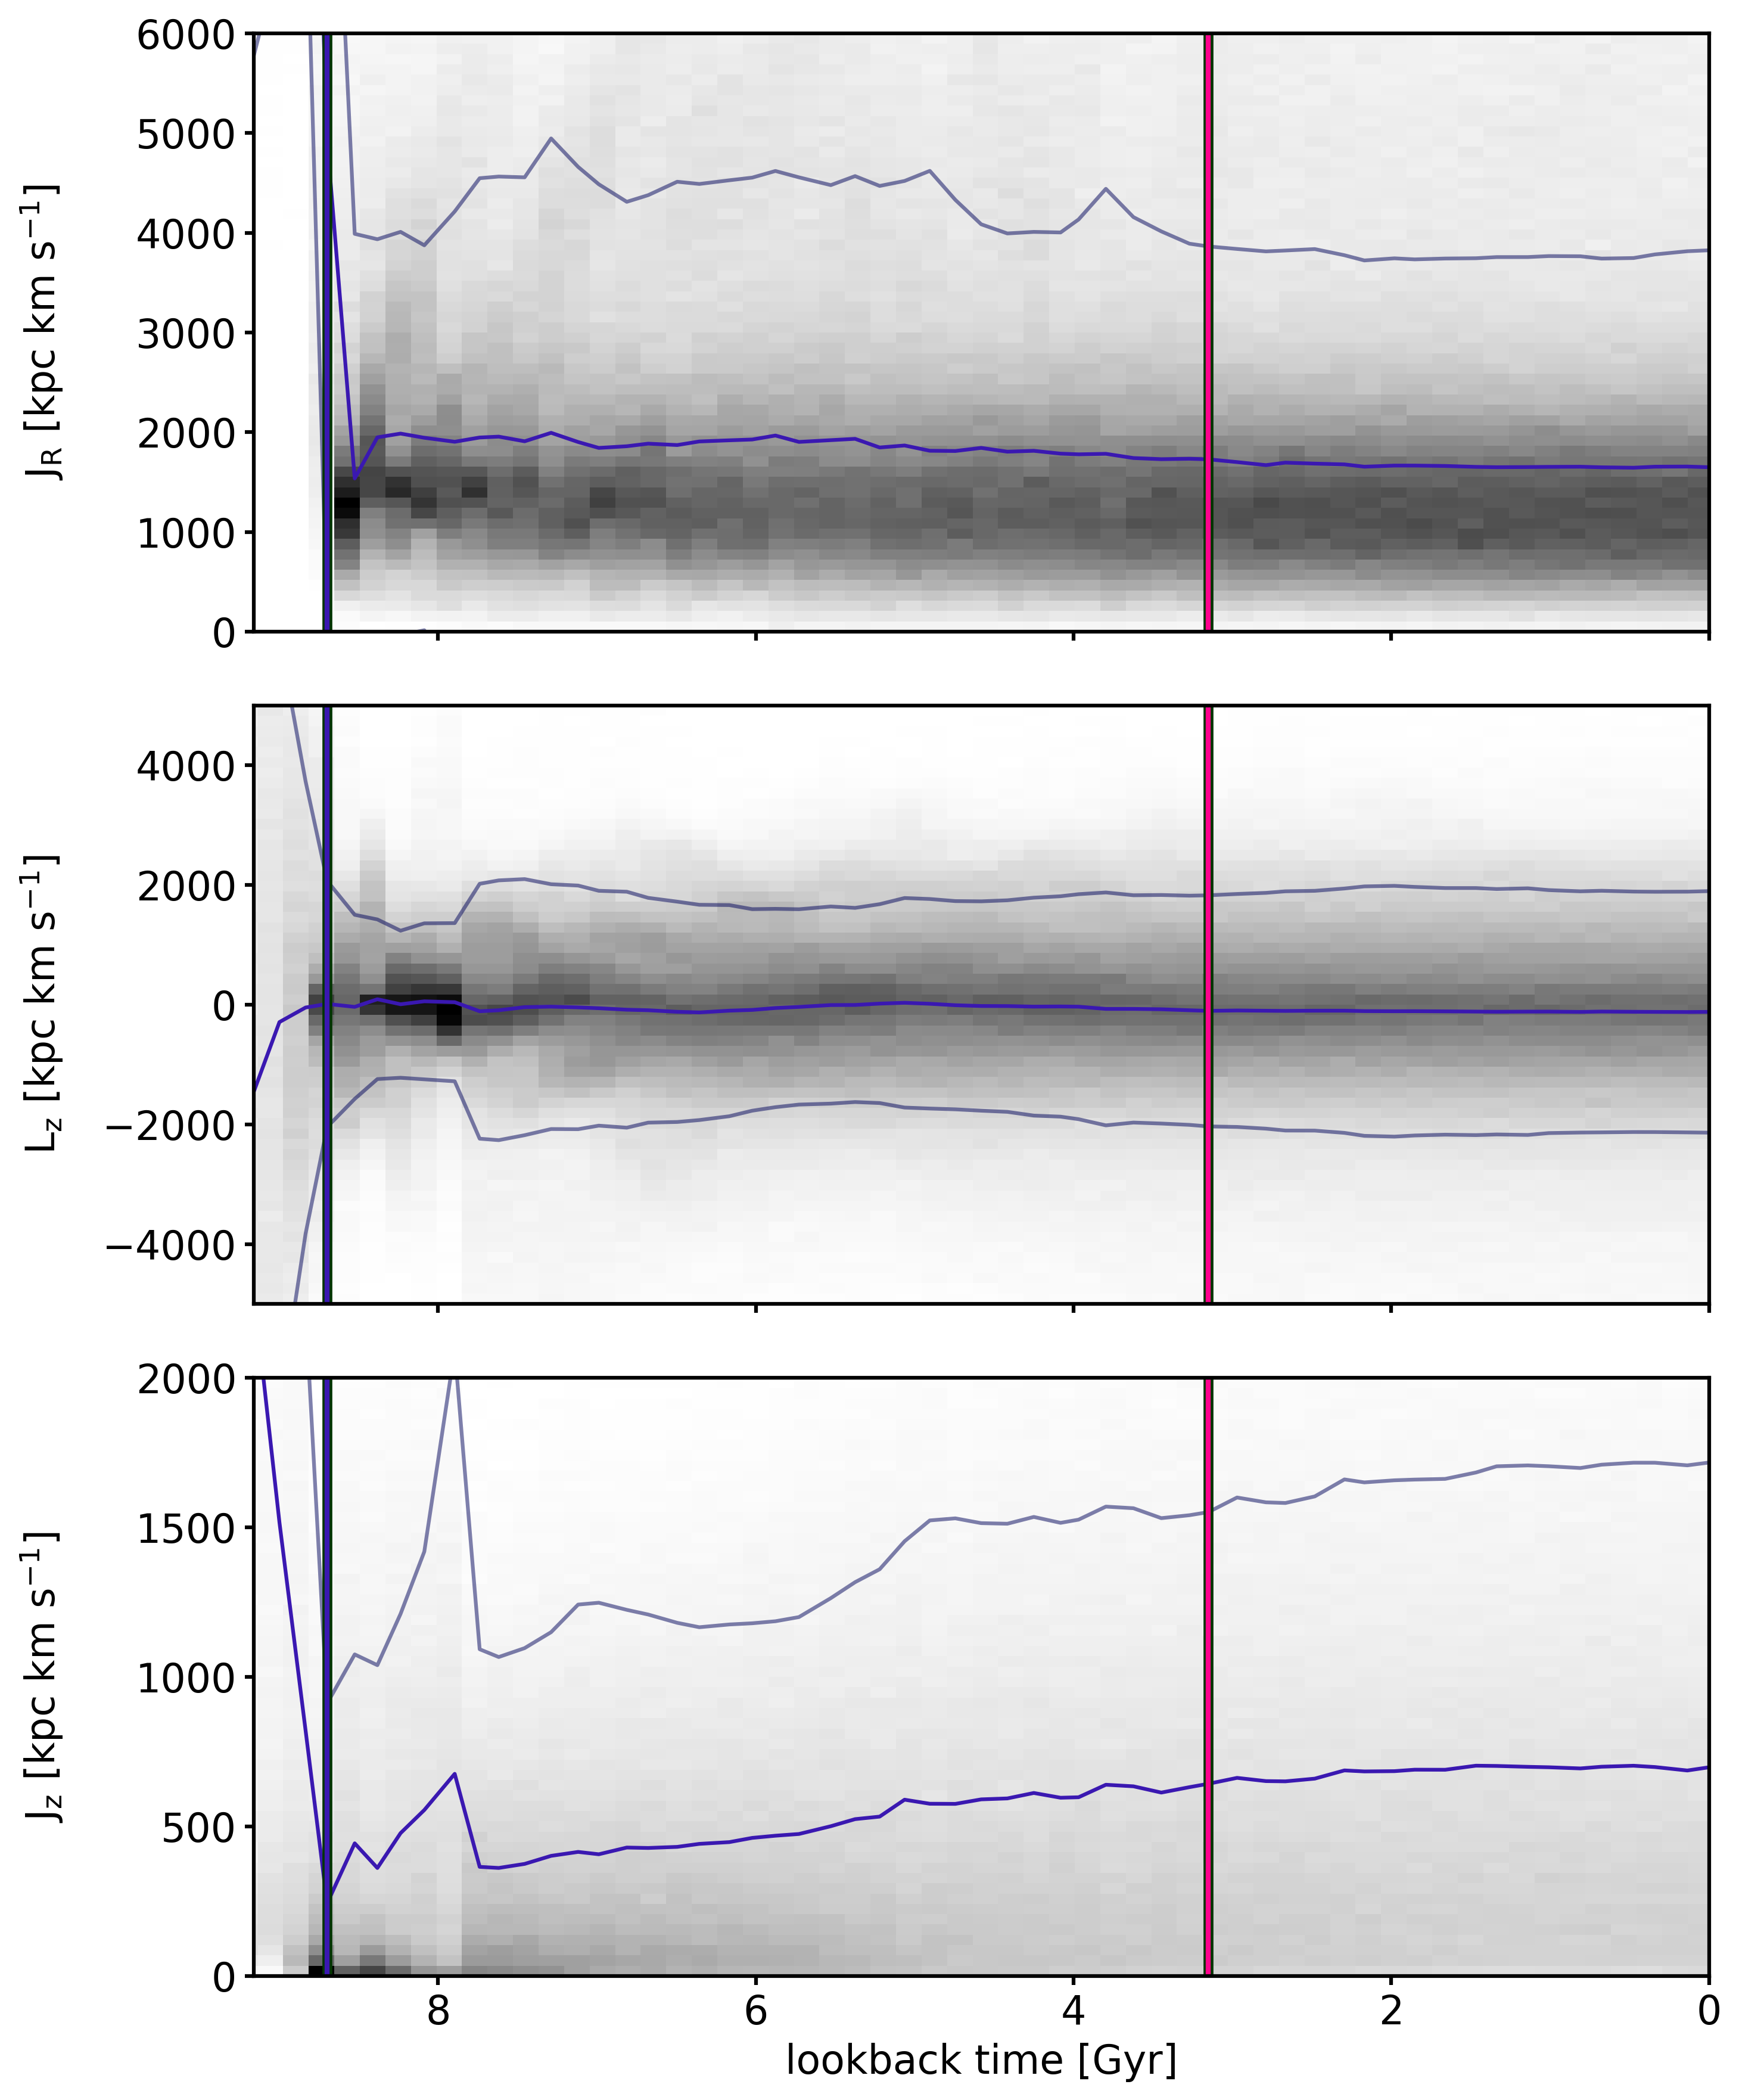
\includegraphics[width=\textwidth]{plots/Dynamics/prog3/action_time_evolution_wodisk_hist_mean.png}
\caption{Time evolution of actions of prog3. The vertical pink and blue lines indicate times of the mergers of prog2 and prog3, respectively. The other blue lines are the median and the standard deviation. The panels are the same as in Figure \ref{fig:actions_time_evolution_prog2}. During the merger of prog3, $\overline{J}_z$ and $\sigma{_J_z}$ minimize. At that time, disk and halo parameters of the potential change slopes (see Figure \ref{fig:pot_val_evol}), probably caused by this merger. Shortly after the merger, the spread in $J_R$ and in $L_z$ minimizes while at the same time the median of $J_z$ and $\sigma{_J_z}$ rise steeply. The following evolution is rather constant for all actions with the spread slowly increasing.}\label{fig:actions_time_evolution_prog3}
\end{figure}

\begin{figure}[htbp]
\captionsetup{format=plain}
    \centering
	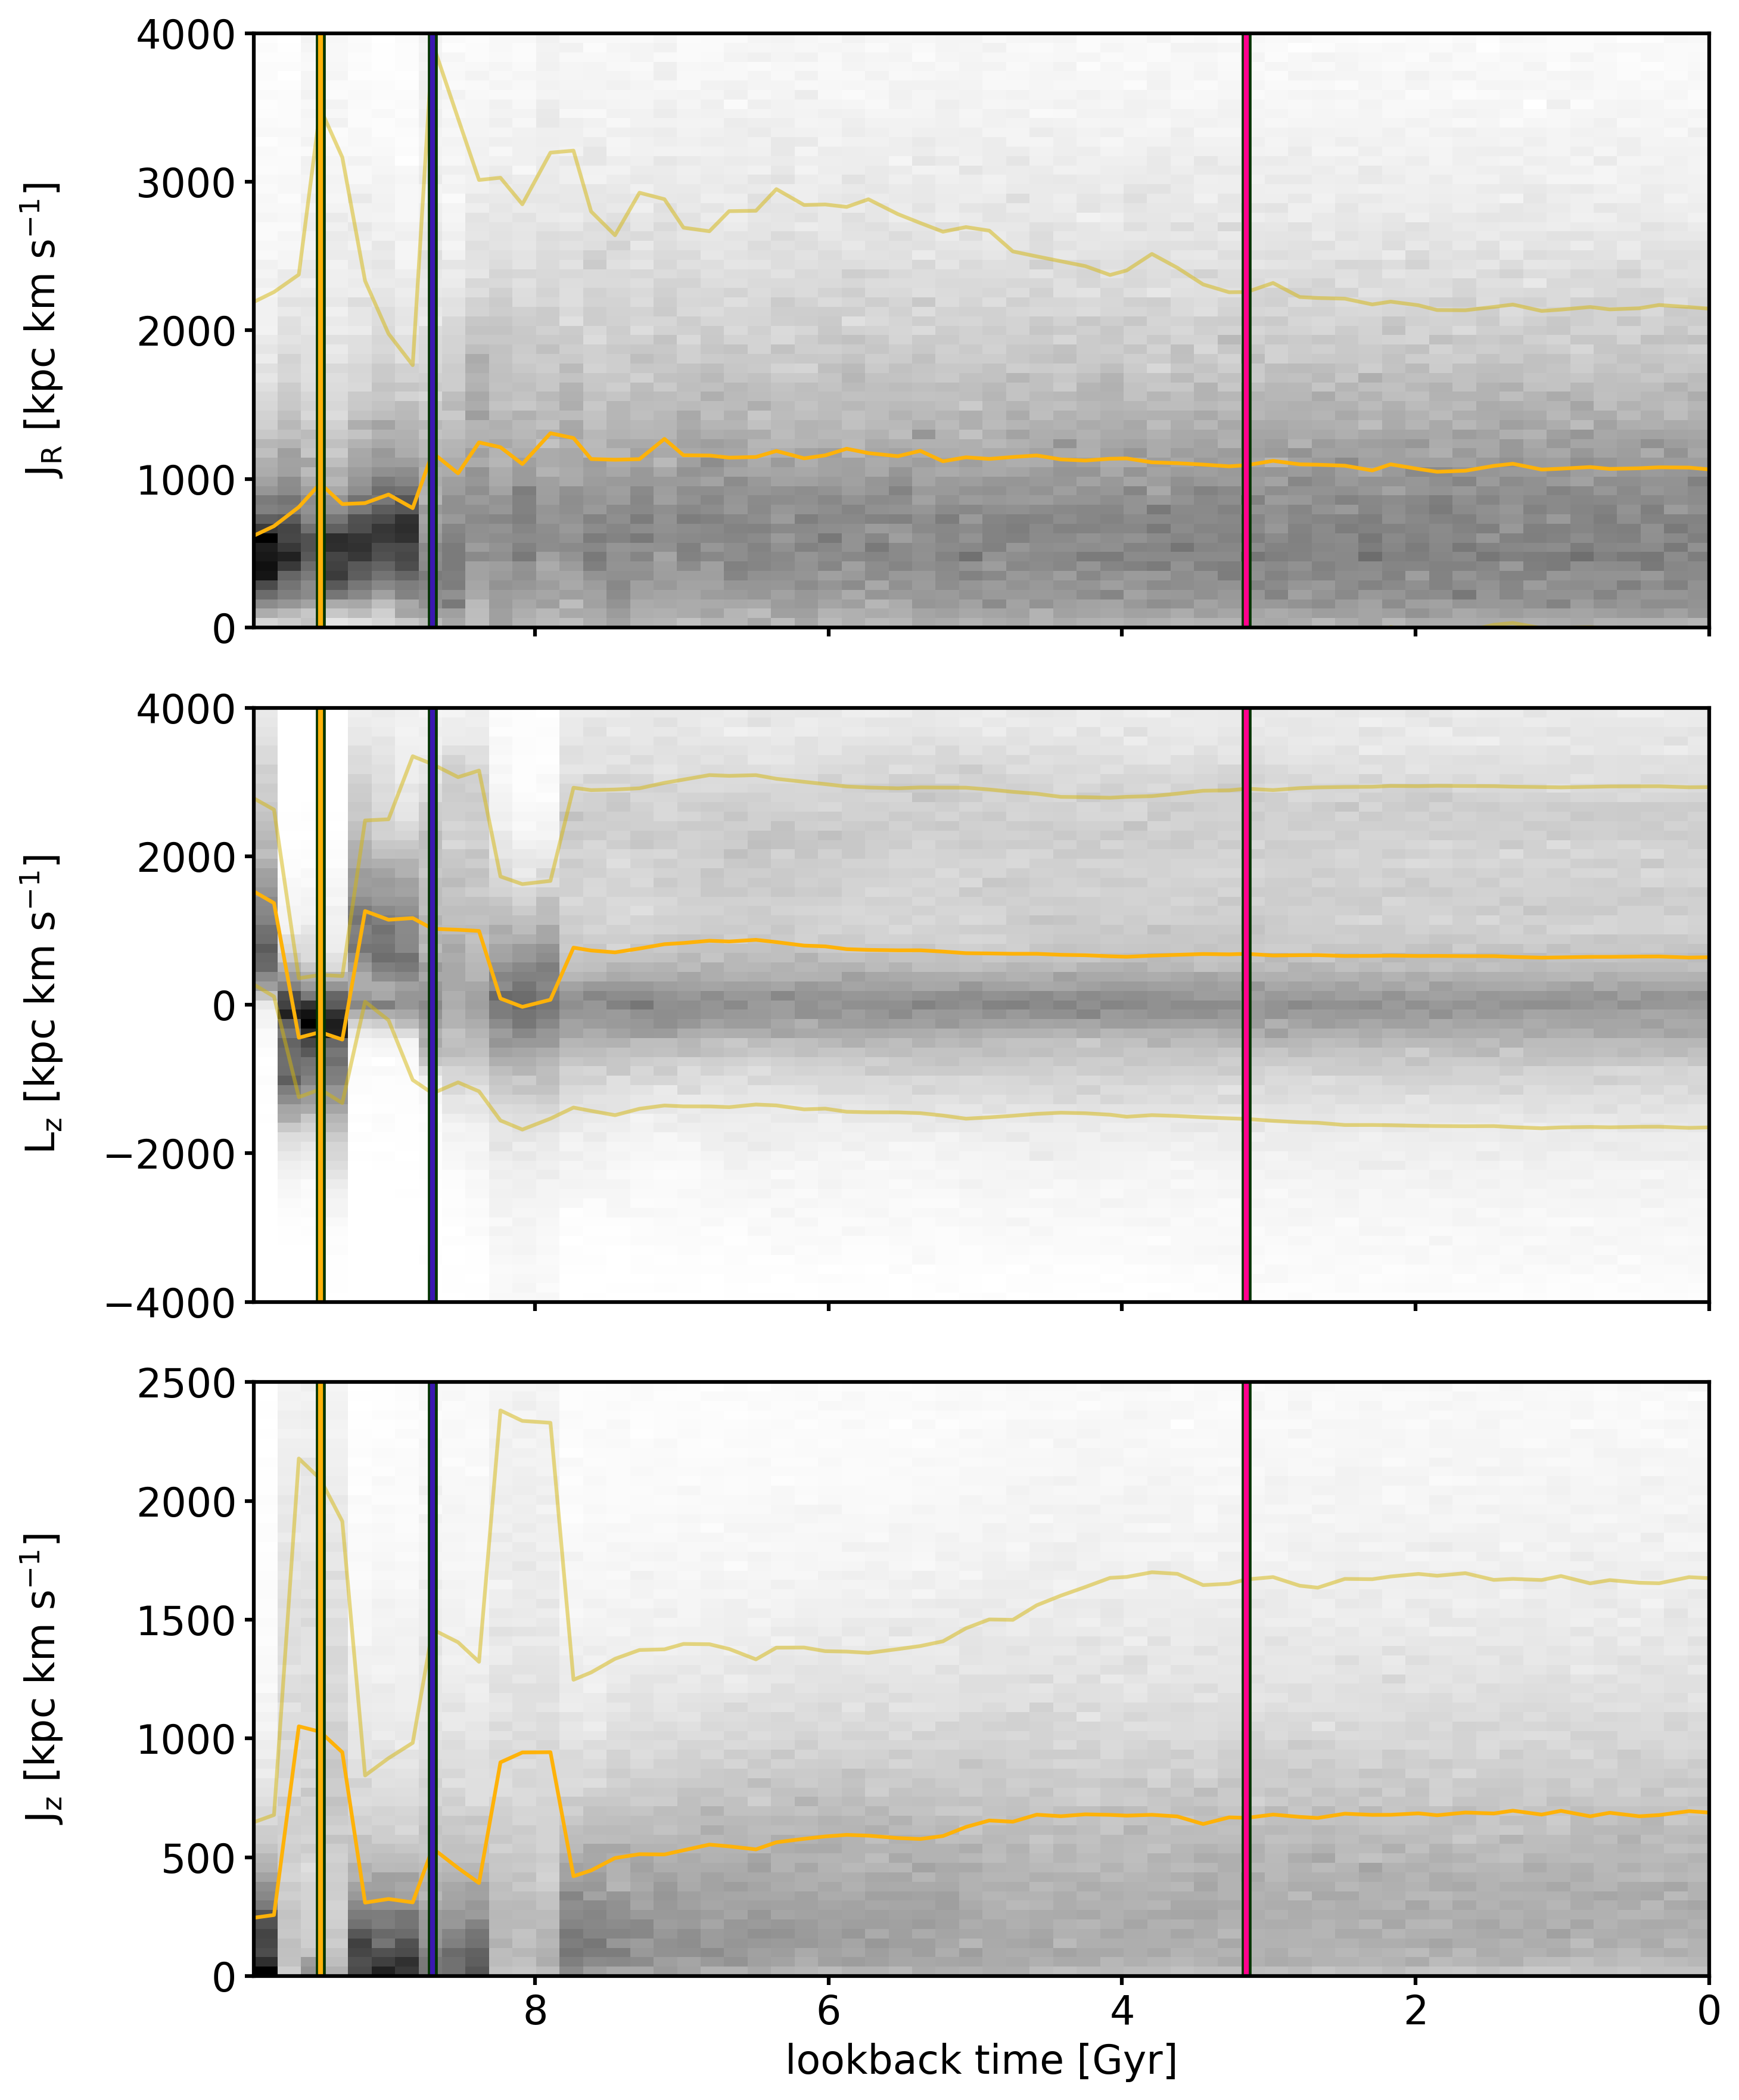
\includegraphics[width=\textwidth]{plots/Dynamics/prog4/action_time_evolution_wodisk_hist_mean.png}
    \caption{Prog4's \acp{GC} time evolution in action space. The vertical pink, blue and yellow lines indicate times of the mergers of prog2, prog3 and prog4, respectively. The yellow lines are median and standard deviation. The panels are the same as in Figure \ref{fig:actions_time_evolution_prog2}. During the merger of prog4, radial and vertical actions have a steep rise while $L_z$ drops below 0. Something similar happens shortly after the merger of prog3. Since \SI{7.5}{Gyr} the actions stay constant and with the merger of prog2, the scatter in $J_R$ and $J_z$ becomes even less, is, however, still very large.}\label{fig:actions_time_evolution_prog4}
\end{figure}
In Figures \ref{fig:actions_time_evolution_prog2}, \ref{fig:actions_time_evolution_prog3} and \ref{fig:actions_time_evolution_prog4} we present these time evolutions for the \acp{GC} of prog2 / prog3 / prog4, respectively. For the prog2 \acp{GC}, Figure \ref{fig:actions_time_evolution_prog2}, we see nicely how before the merger the actions where very widely spread and towards the merger and especially afterwards their variance becomes smaller and the mean of each action stays constant. Since the merger, more significant clumping than in the last snapshot is not seen. In prog3, we find a strong clump shortly after the merger. The actions of prog4 are strongly varying shortly after the merger for about \SI{2}{Gyr} before they become steady.

\subsubsection{Mean best fit potential}\label{subsubsec:GCs_actions_time_mean_right_pot}
The idea that actions do not change over time is valid in a static or only slowly varying (axisymmetric) potential. Even though the overall action distribution did not change too much over time, we will see in Section \ref{subsec:box_GCs} that individual orbits vary drastically over time. Therefore, we need to test if the assumption of having a potential which only varies slowly is true. A rather simple execution is to calculate the action evolution in a static potential and check if it varies from our results. To do so, we calculate the mean of each potential parameter since the last big merger event (prog2). 
\begin{figure}[htbp]
\captionsetup{format=plain}
    \centering
	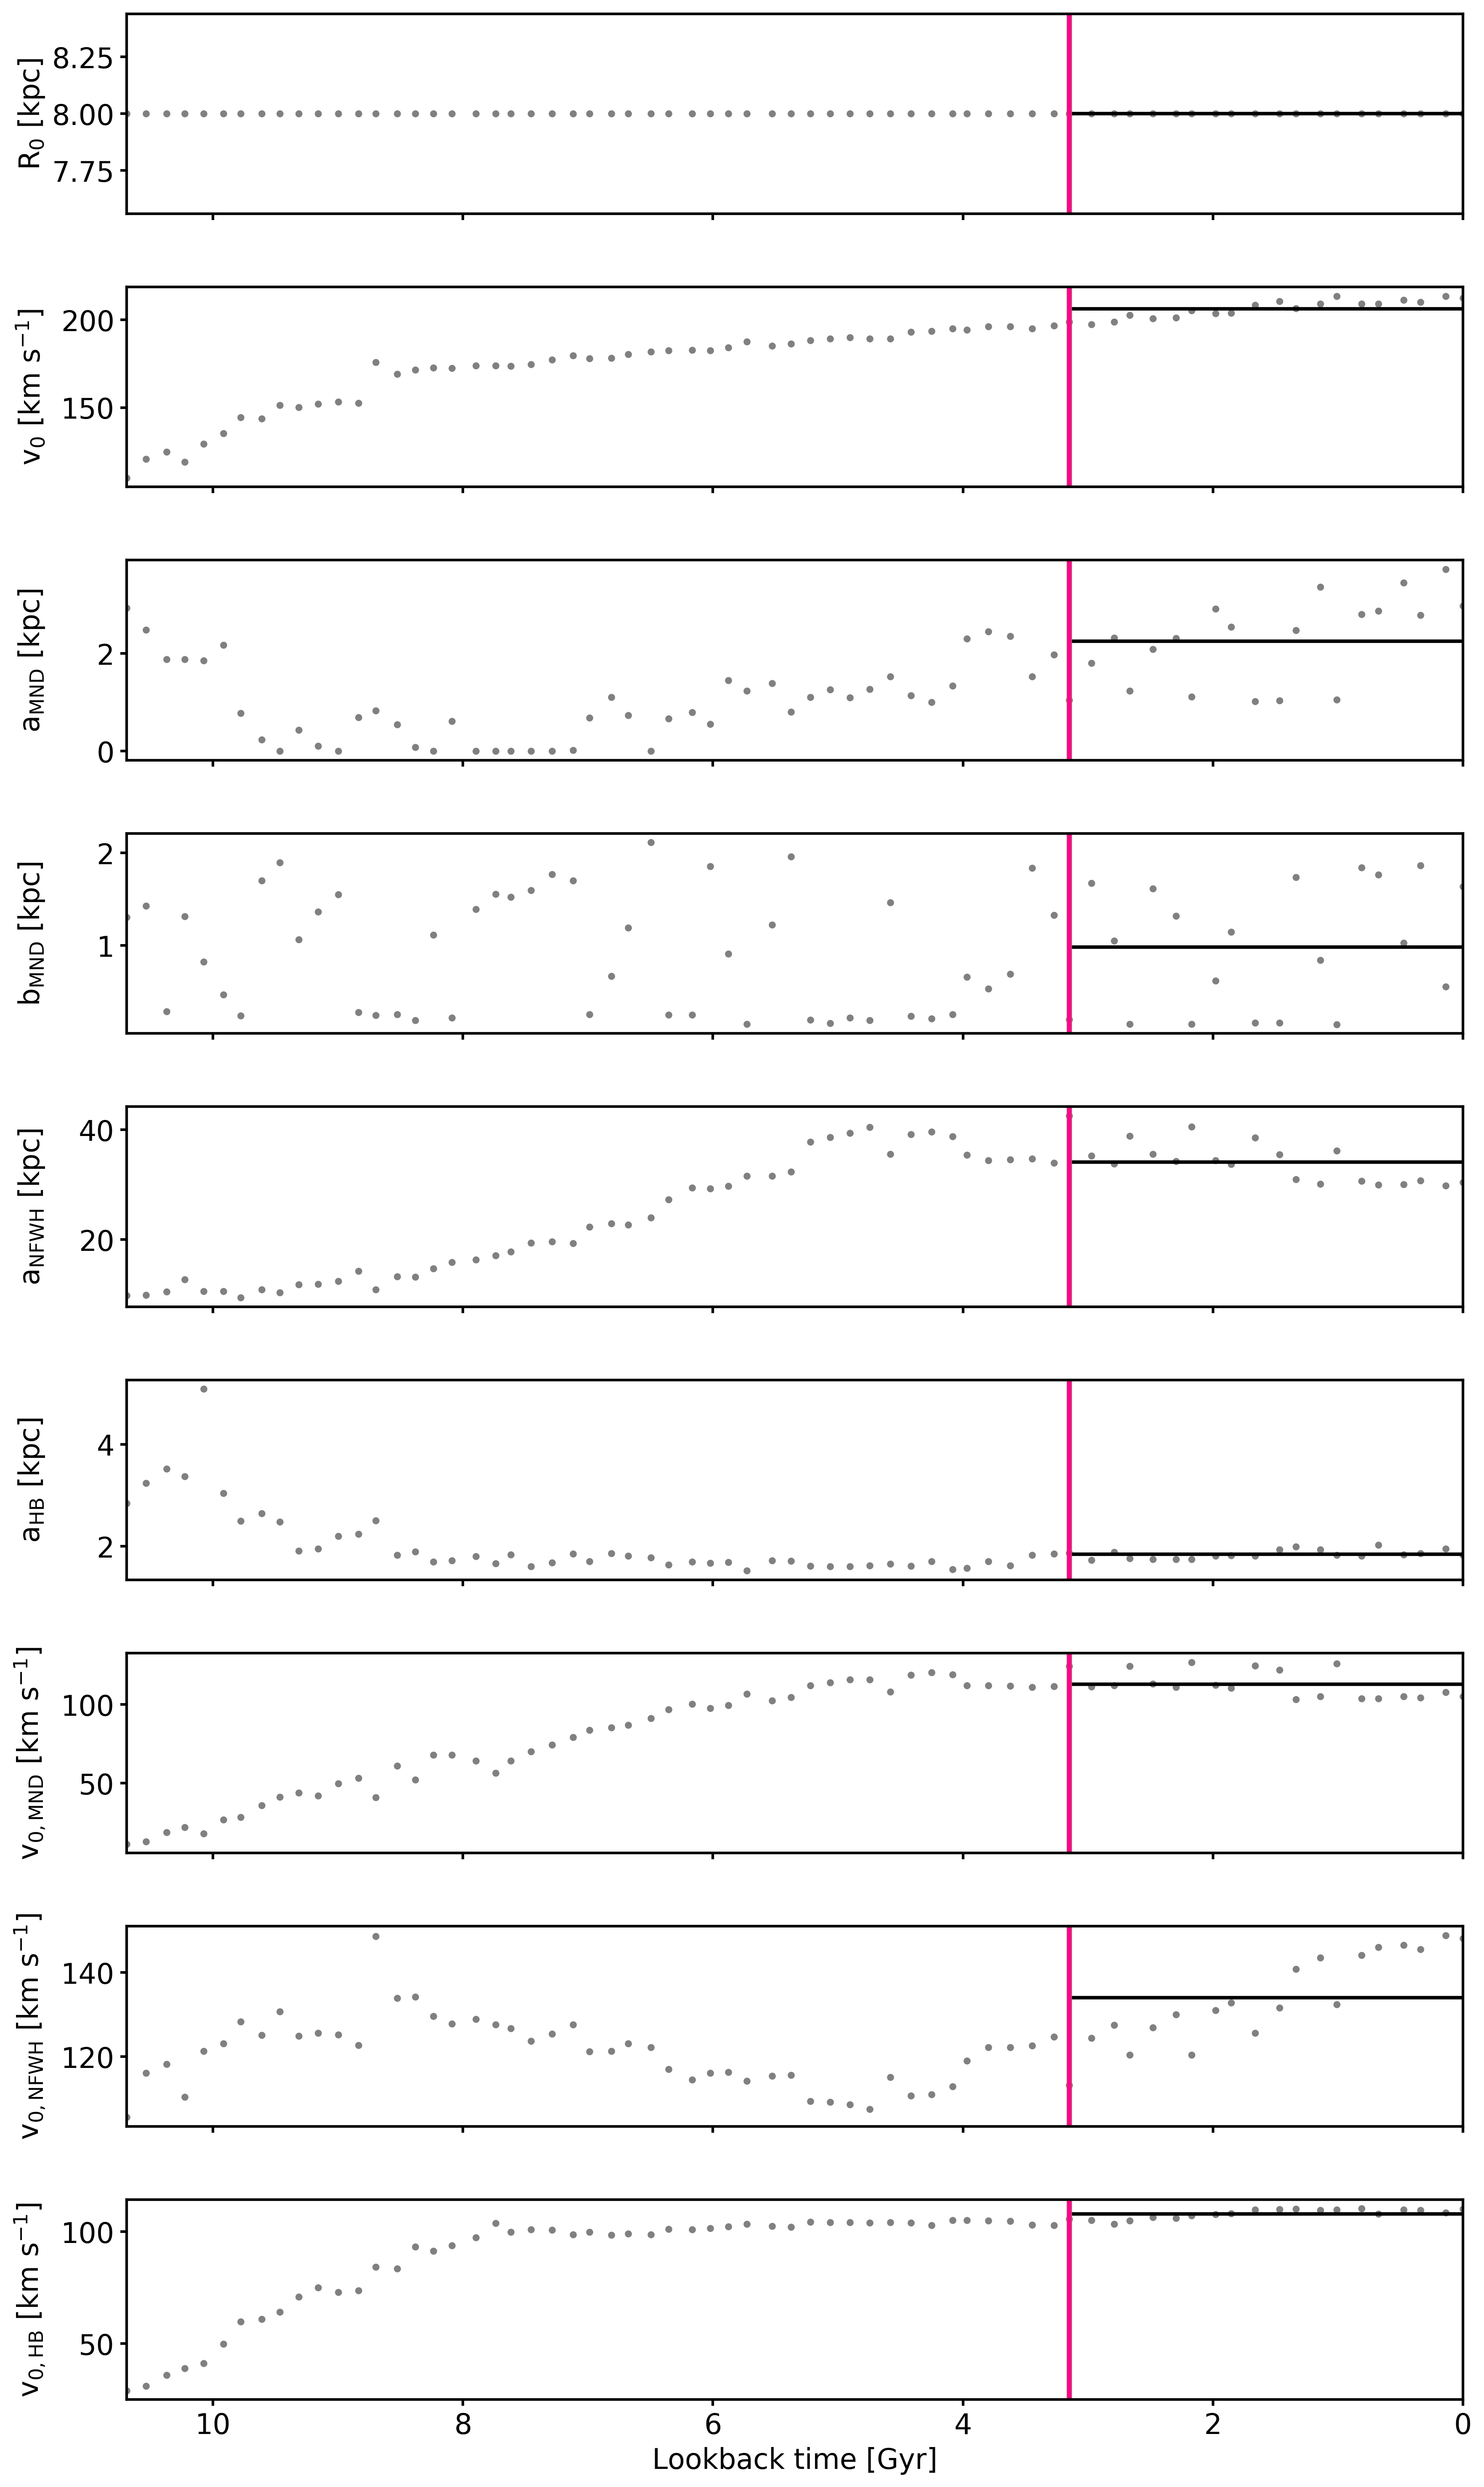
\includegraphics[width=0.8\textwidth]{plots/Dynamics/mean_pot/potential_evolution_with_mean_jan19.png}
    \caption{Time evolution of best fit potential parameters and their mean values since the merger of prog2 (indicated in pink). The scatter of disk and halo parameters is relatively large while the bulge parameters stay constant in this time range. We use the mean potential parameters (indicated as black lines) to compare the actions in the slowly varying potential (Figure \ref{fig:pot_val_evol}) to the actions in this static potential.}\label{fig:potential_mean_evolution}
\end{figure}
\\In Figure \ref{fig:potential_mean_evolution}, we show again the parameter evolution and the mean value for each which we use to set up the static gravitational potential. Since we have large scatter in the disk and halo parameters it is interesting to see if ignoring their variation has any consequences on the action calculation. 
\begin{figure}[htbp]
\captionsetup{format=plain}
    \begin{subfigure}[c]{0.48\textwidth}
    \centering
    	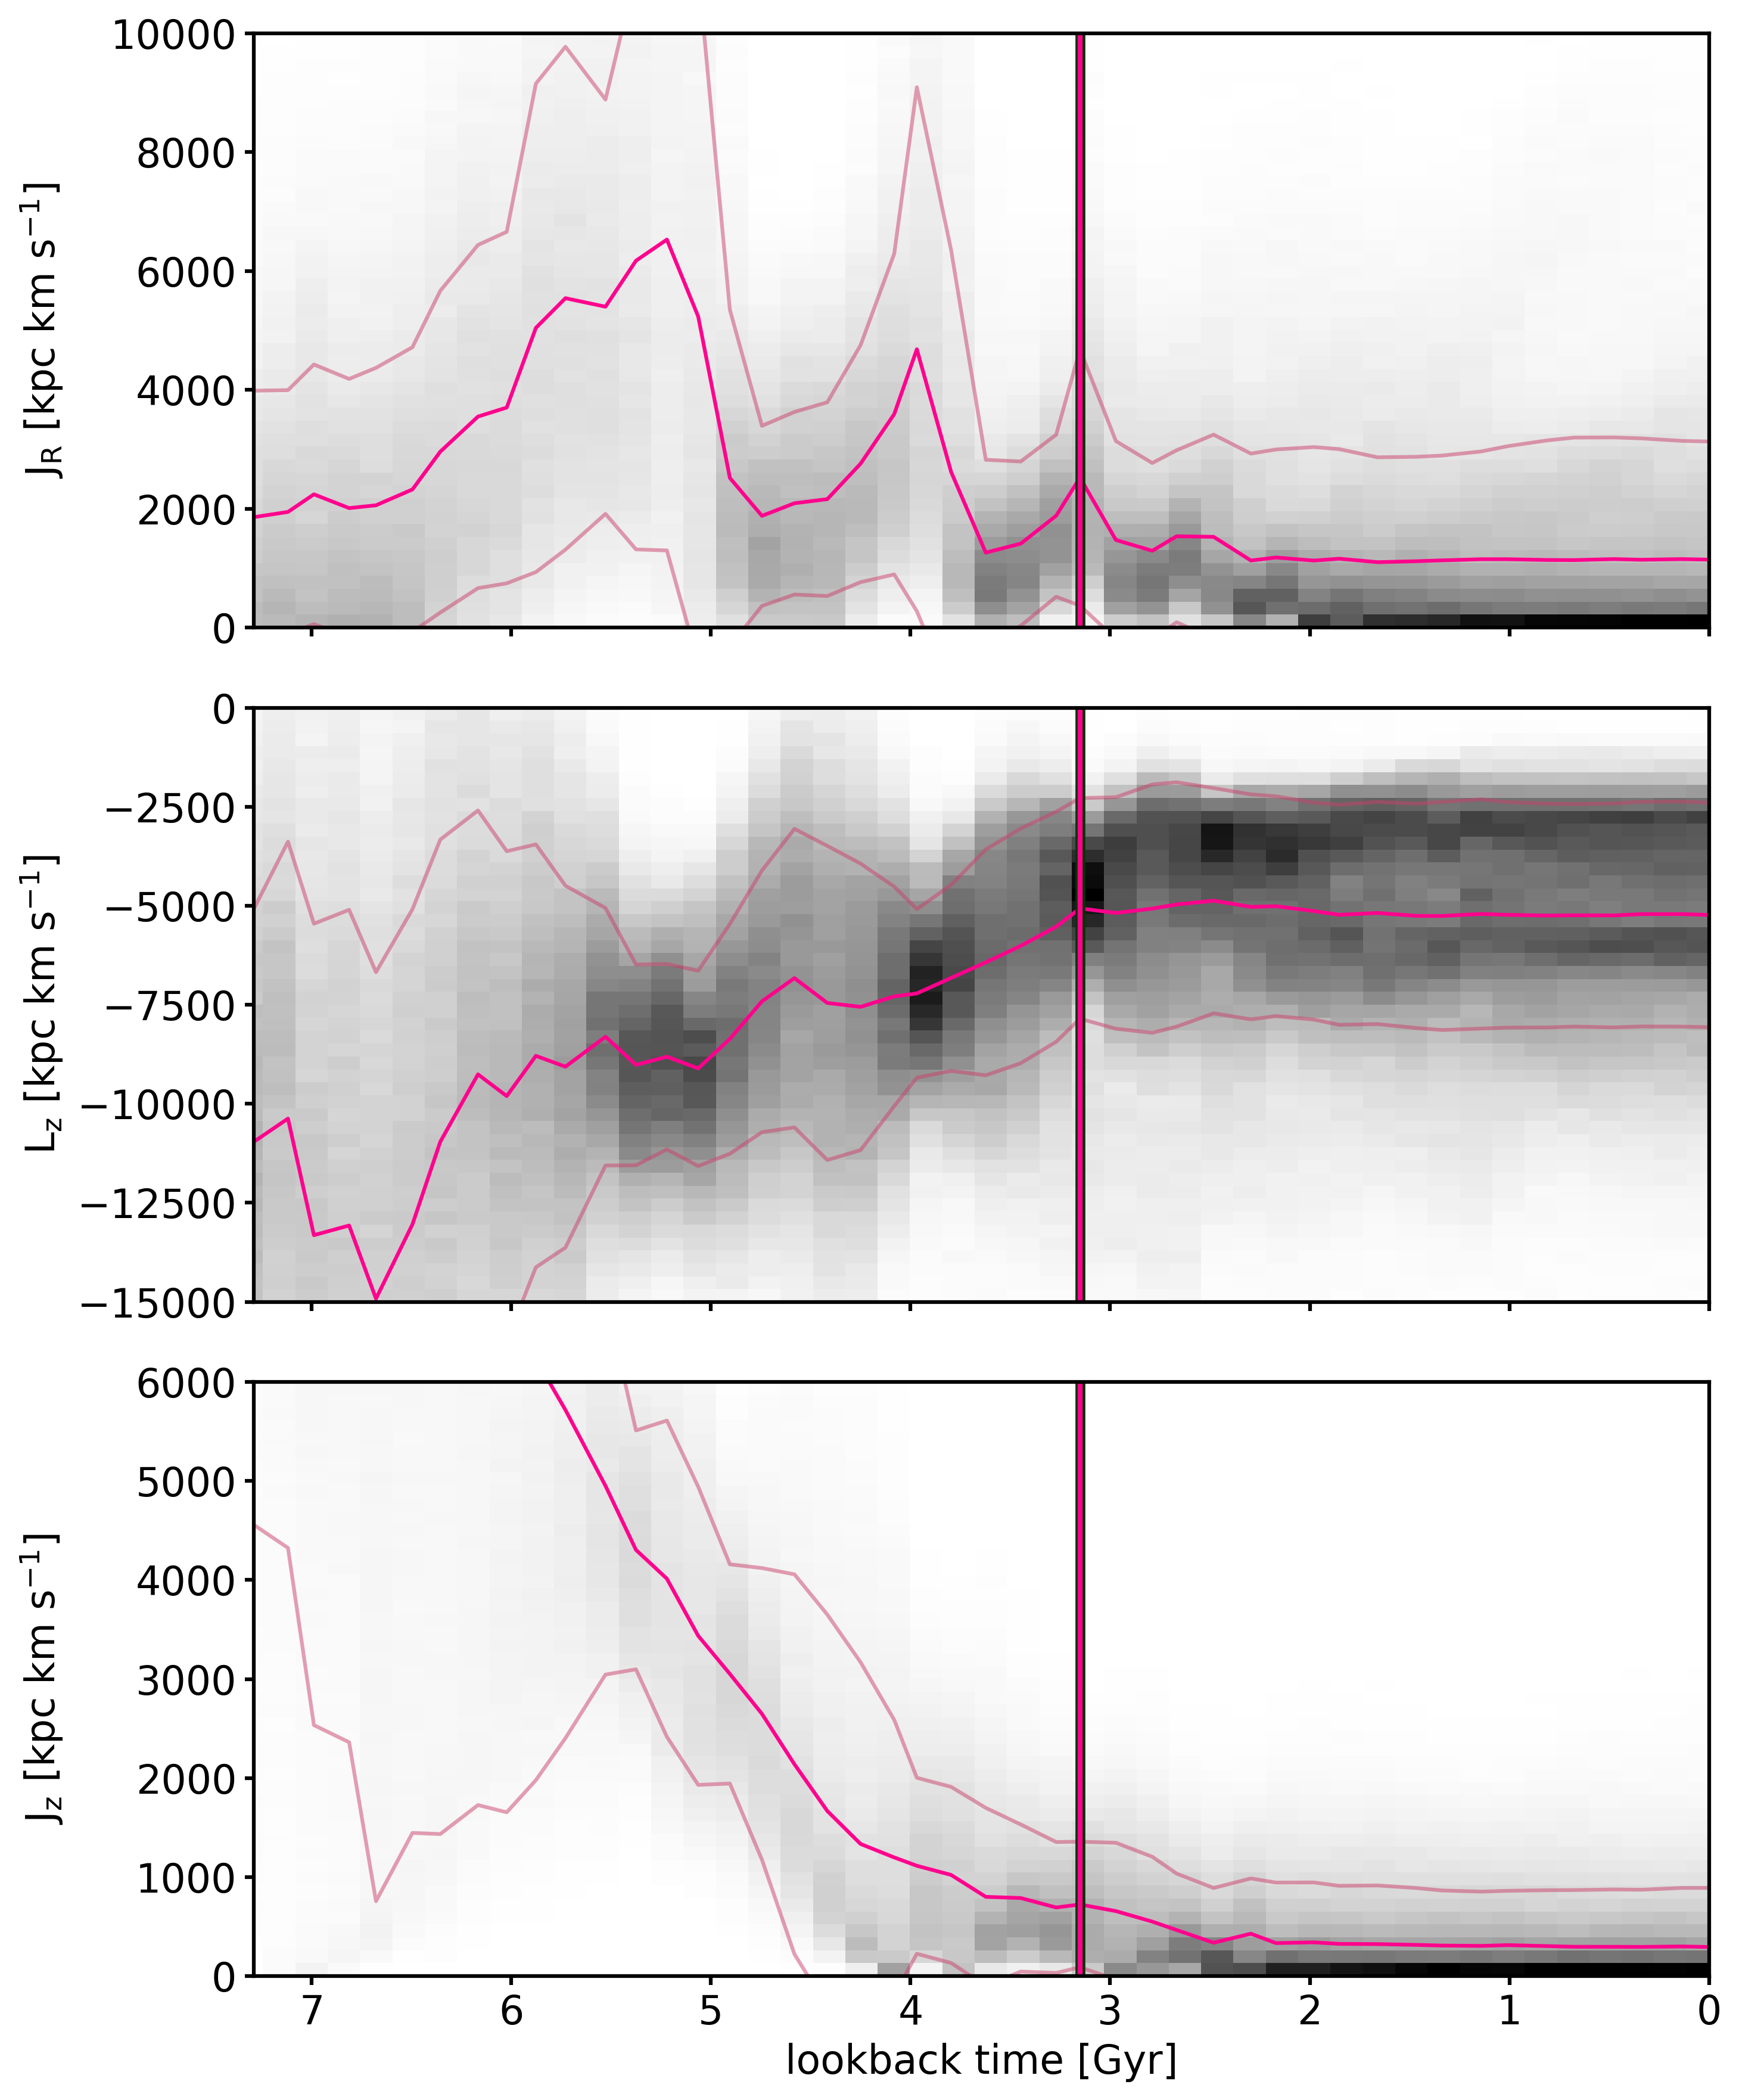
\includegraphics[width=\textwidth]{plots/Dynamics/prog2/action_time_evolution_wodisk_hist_mean.png}
    \end{subfigure}
    ~
    \begin{subfigure}[c]{0.48\textwidth}
    \centering
	    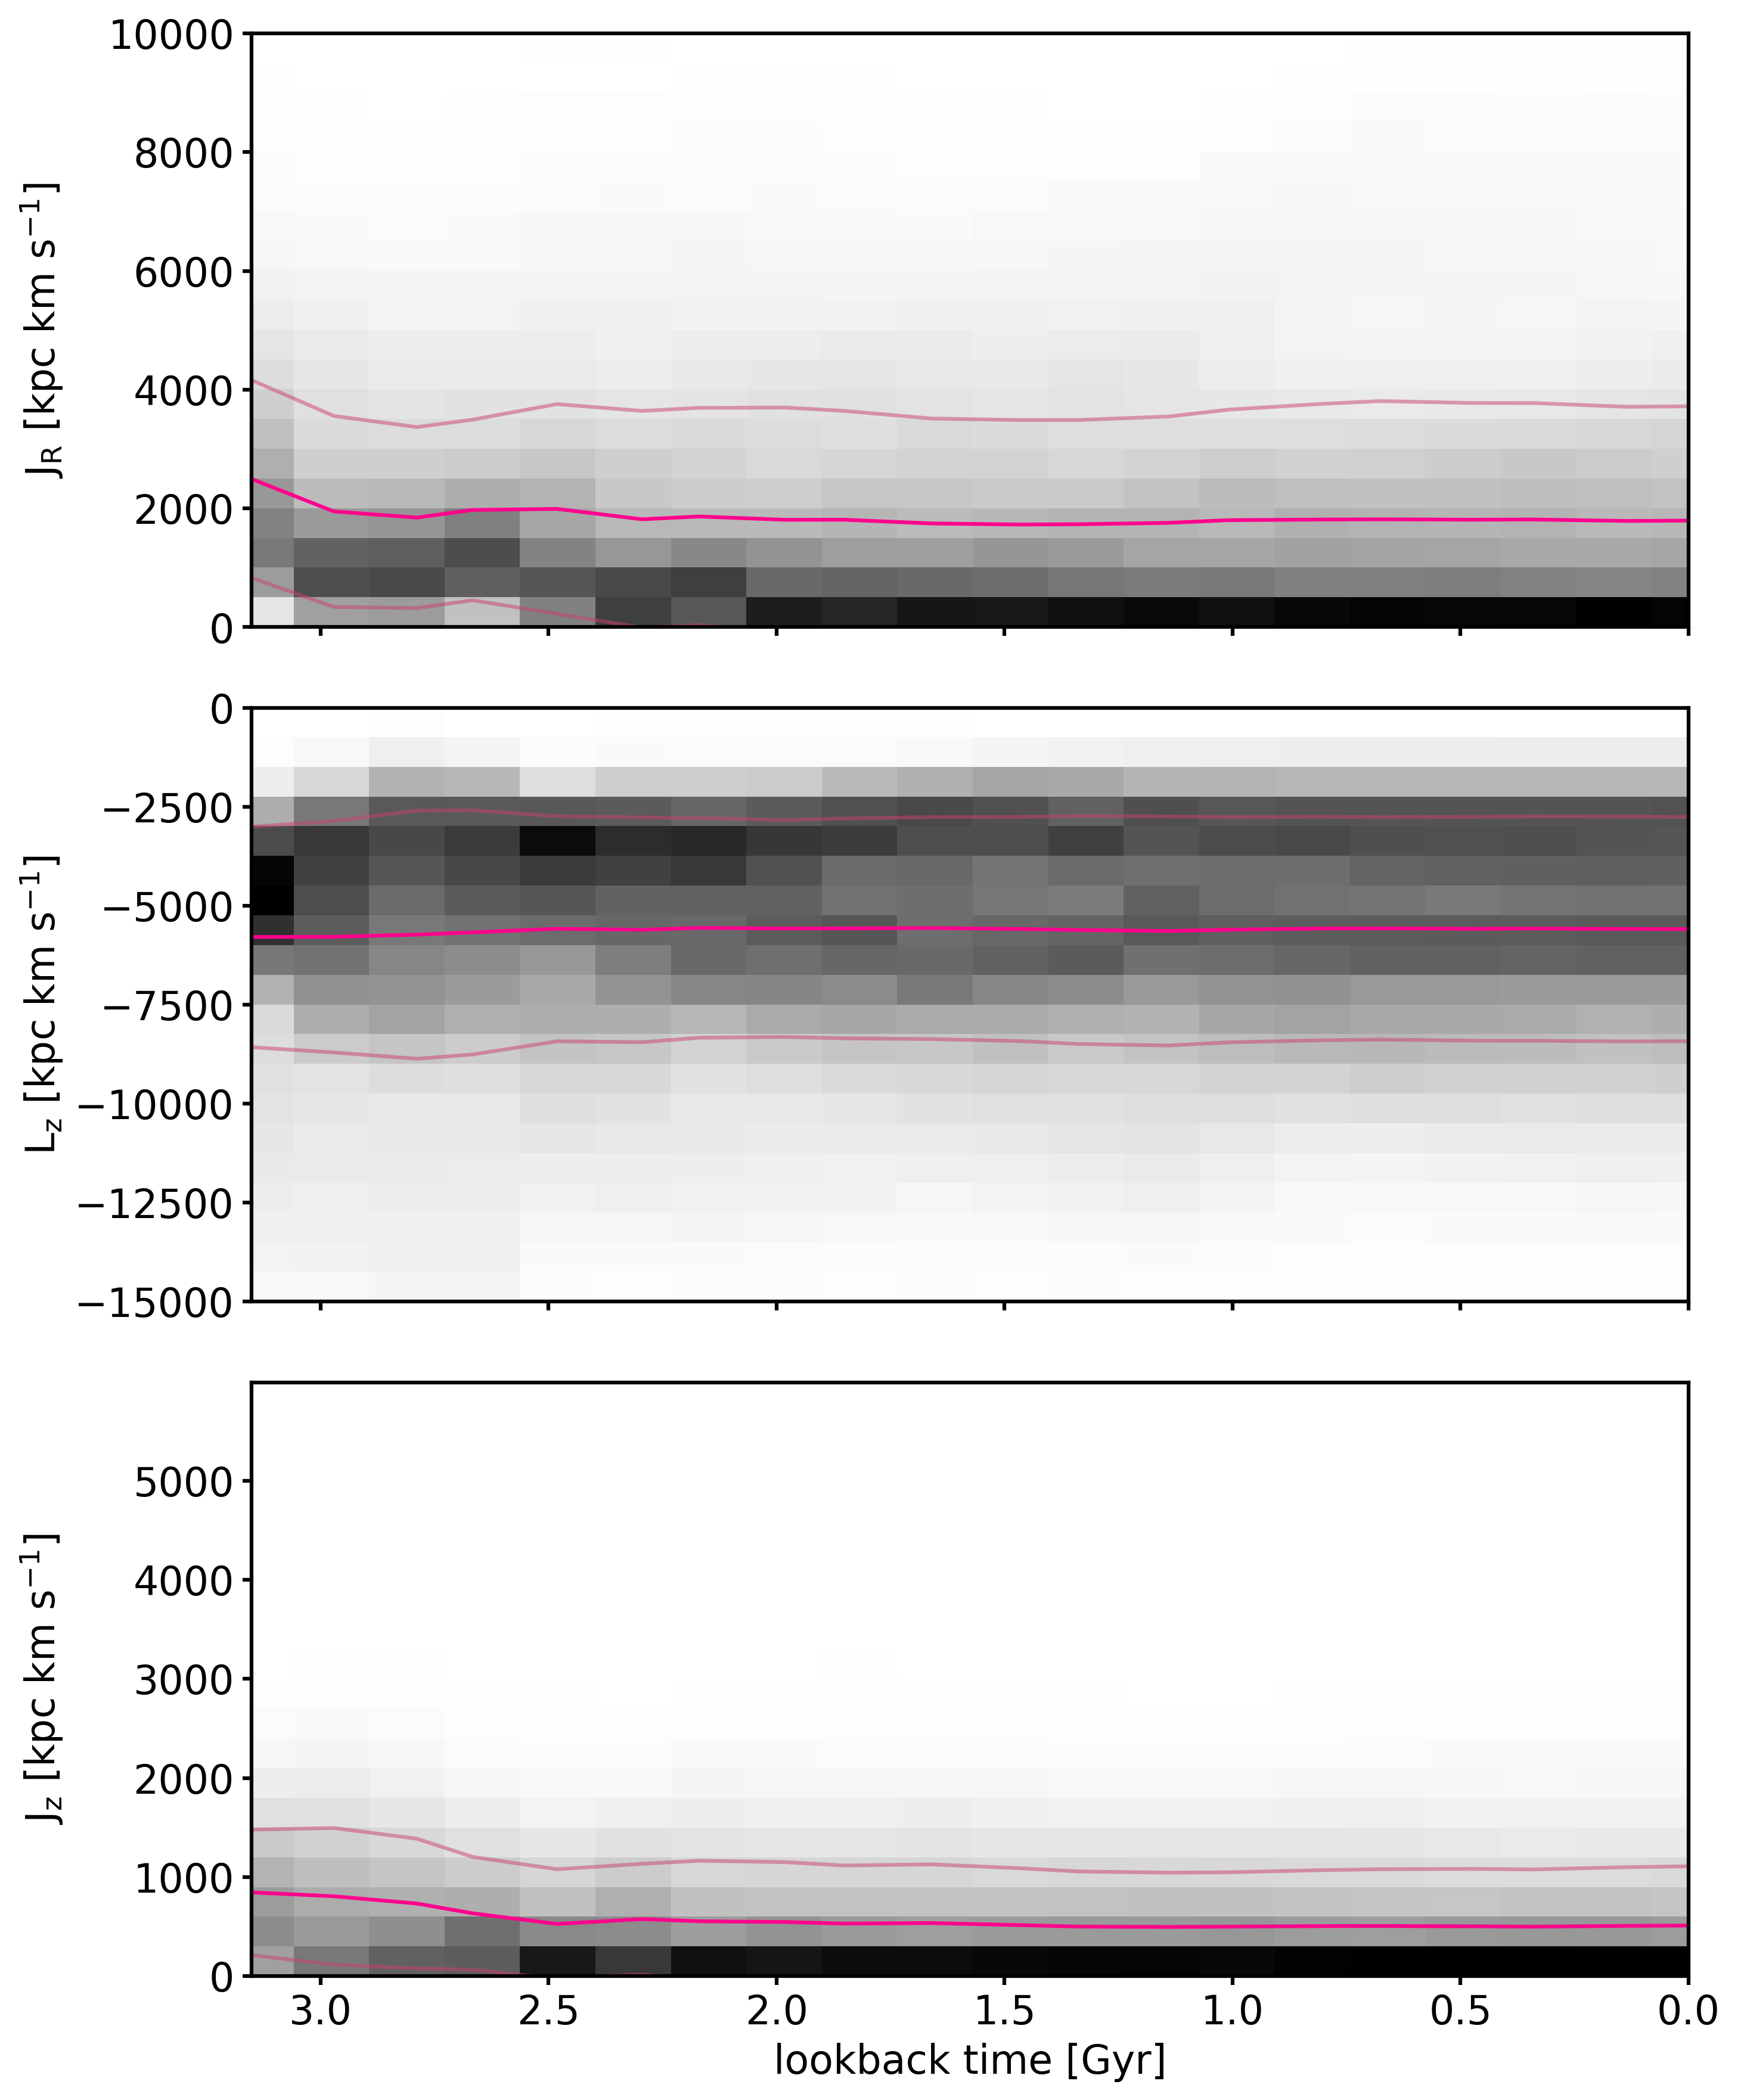
\includegraphics[width=\textwidth]{plots/Dynamics/prog2/action_wodisk_time_evolution_hist_mean_static_pot.png}
    \end{subfigure}
    \caption{Action evolution of prog2. \textit{Left panel:} same as Figure \ref{fig:actions_time_evolution_prog2}. \textit{Right panel:} Action evolution of prog2 since its merger in a constant potential with parameters given in Figure \ref{fig:potential_mean_evolution}. $\overline{J_R}$ and $\overline{J_z}$ are a slightly larger in the constant potential. The standard deviations and the slopes of the evolution stay the same.}\label{fig:comparison_actions_time_evolution_mean_pot_prog2}
\end{figure}
In the time regime since the last merger we calculated the actions of each progenitor group in the static potential. In Figure \ref{fig:comparison_actions_time_evolution_mean_pot_prog2}, we compare the \acp{GC} of prog2 in action space in the varying potential (left) and the static potential (right). There is no difference in the time evolution visible after the merger. We did the same for the \acp{GC} of prog3 and prog4 and they also show no differences. Therefore, the assumption of having a slowly evolving potential can be considered as satisfied.
\iffalse
\begin{figure}
\captionsetup{format=plain}
    \centering
	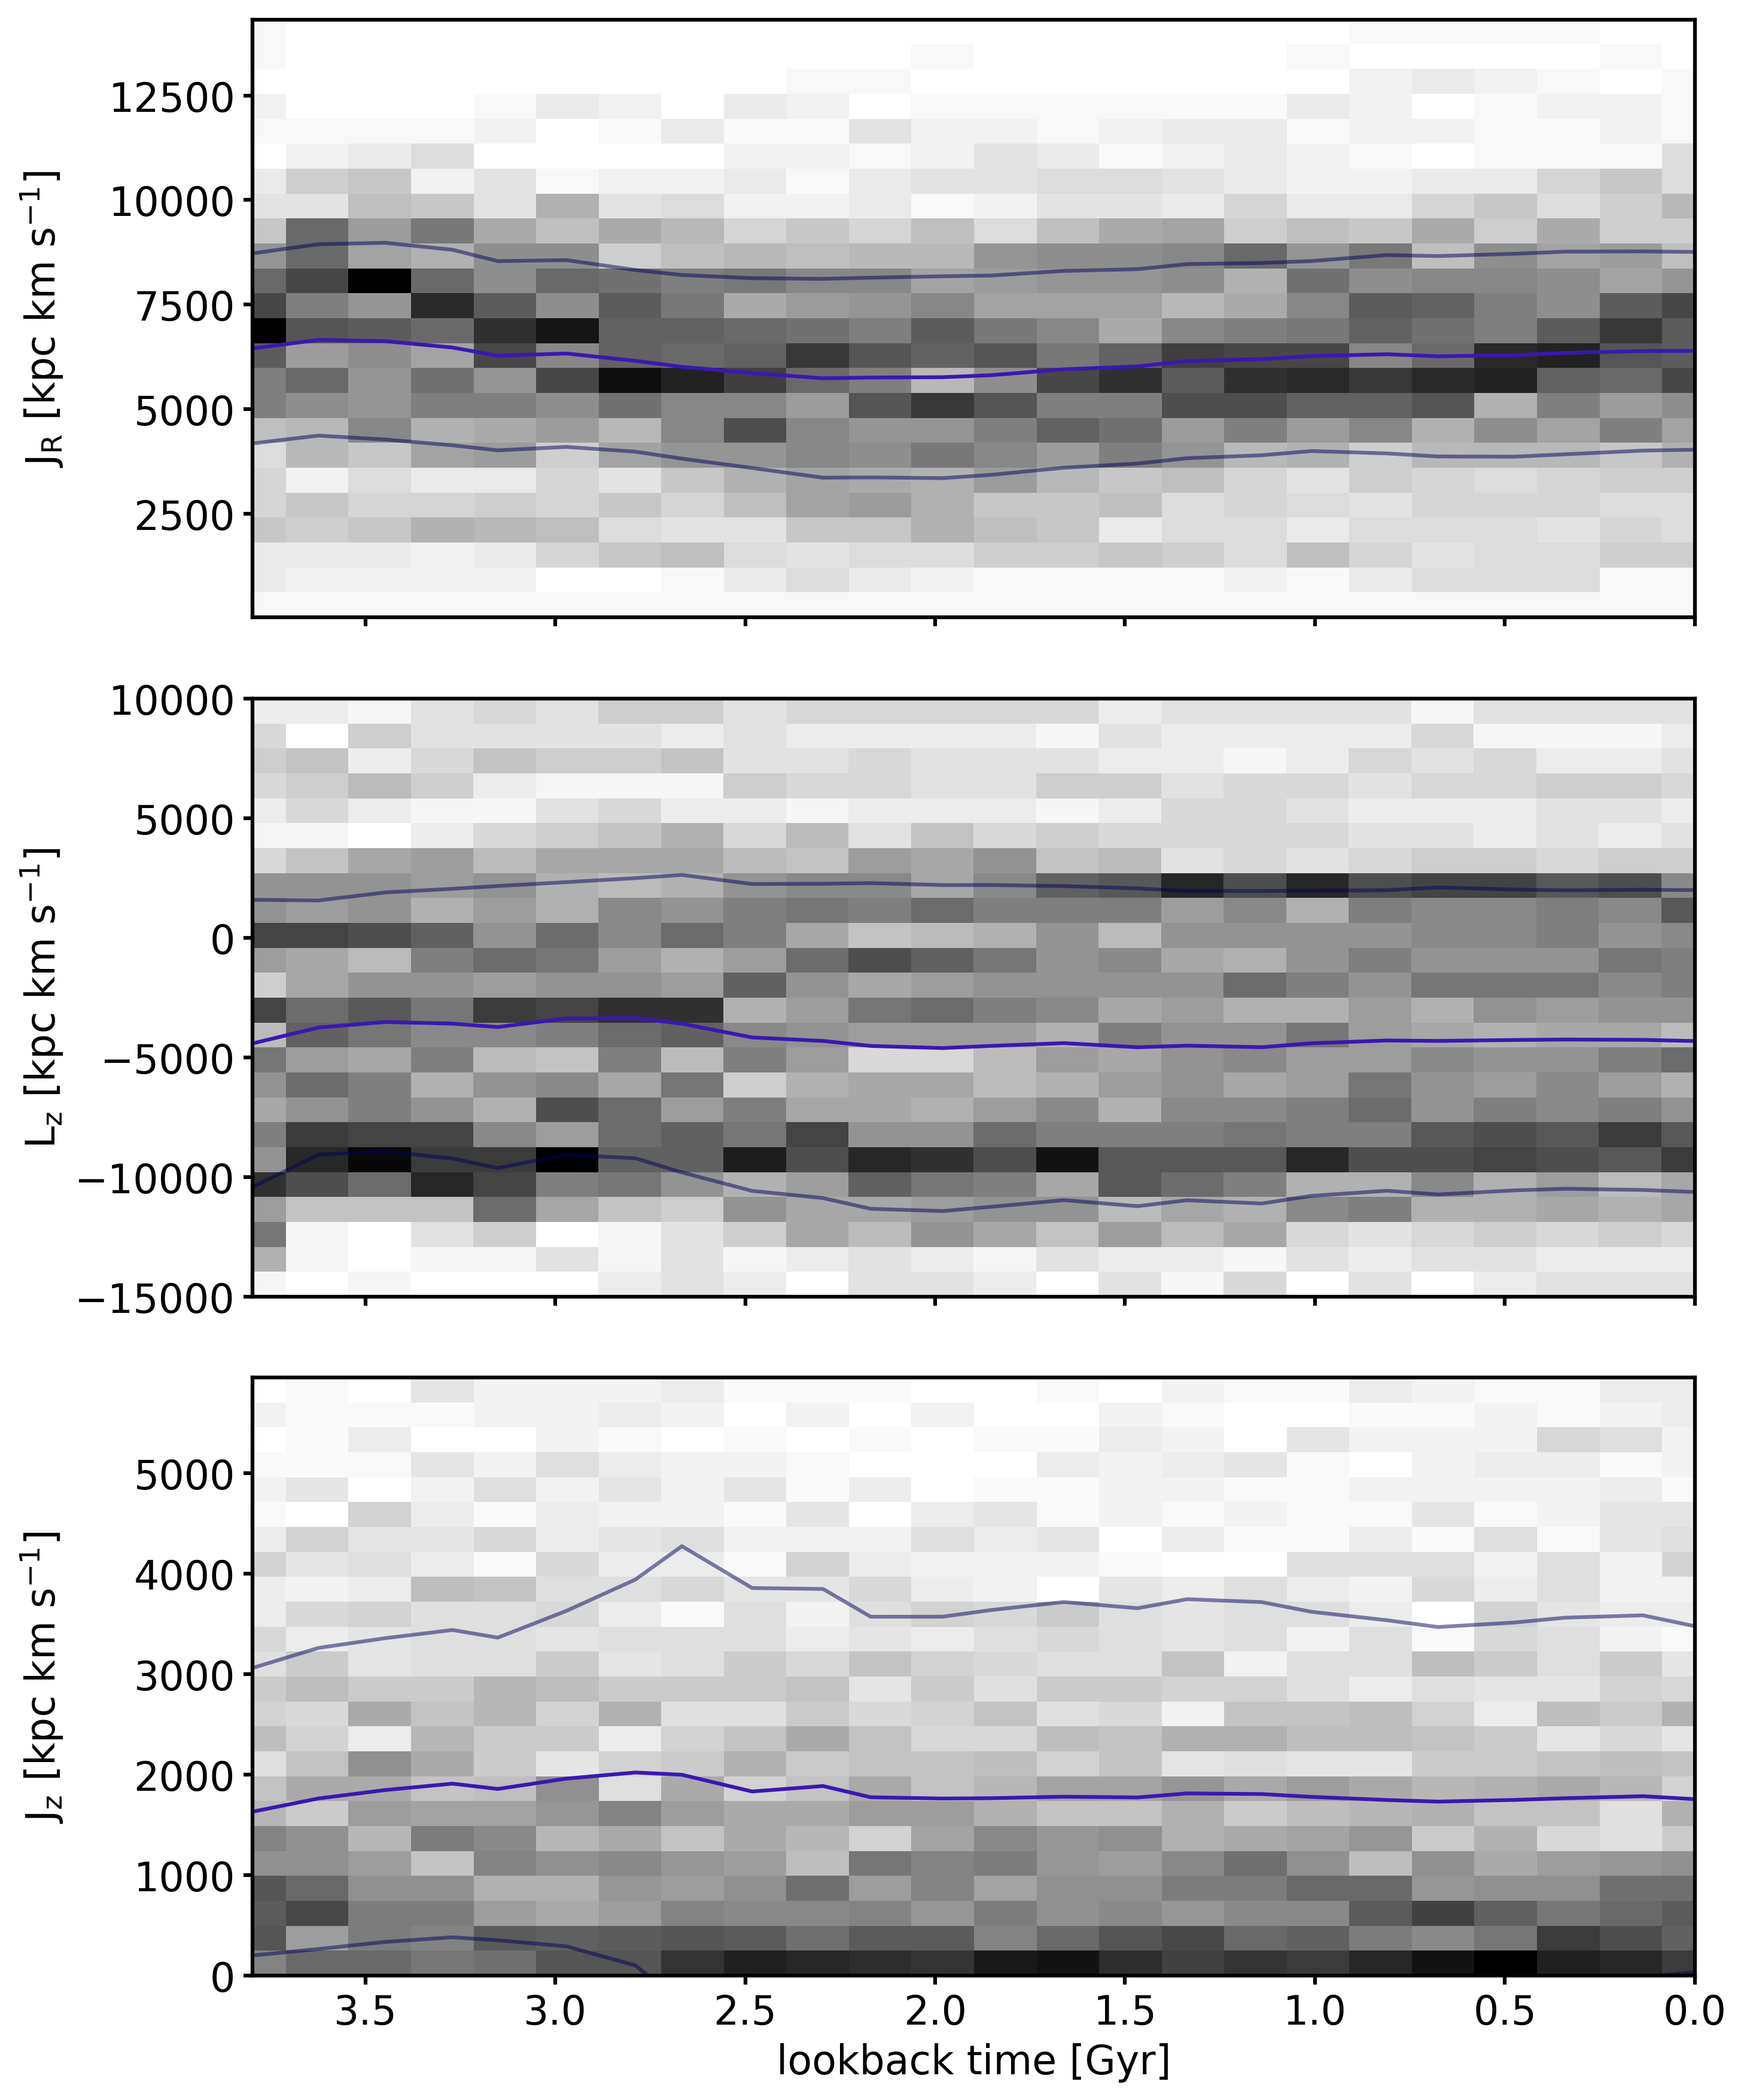
\includegraphics[width=\textwidth]{plots/Dynamics/mean_pot/action_time_evolution_hist_mean_prog3.png}
    \caption{Same as Figure \ref{fig:actions_time_evolution_prog3}, only for a constant potential since the merger of prog2.}\label{fig:actions_time_evolution_mean_pot_prog3}
\end{figure}

\begin{figure}[htbp]
\captionsetup{format=plain}
    \centering
	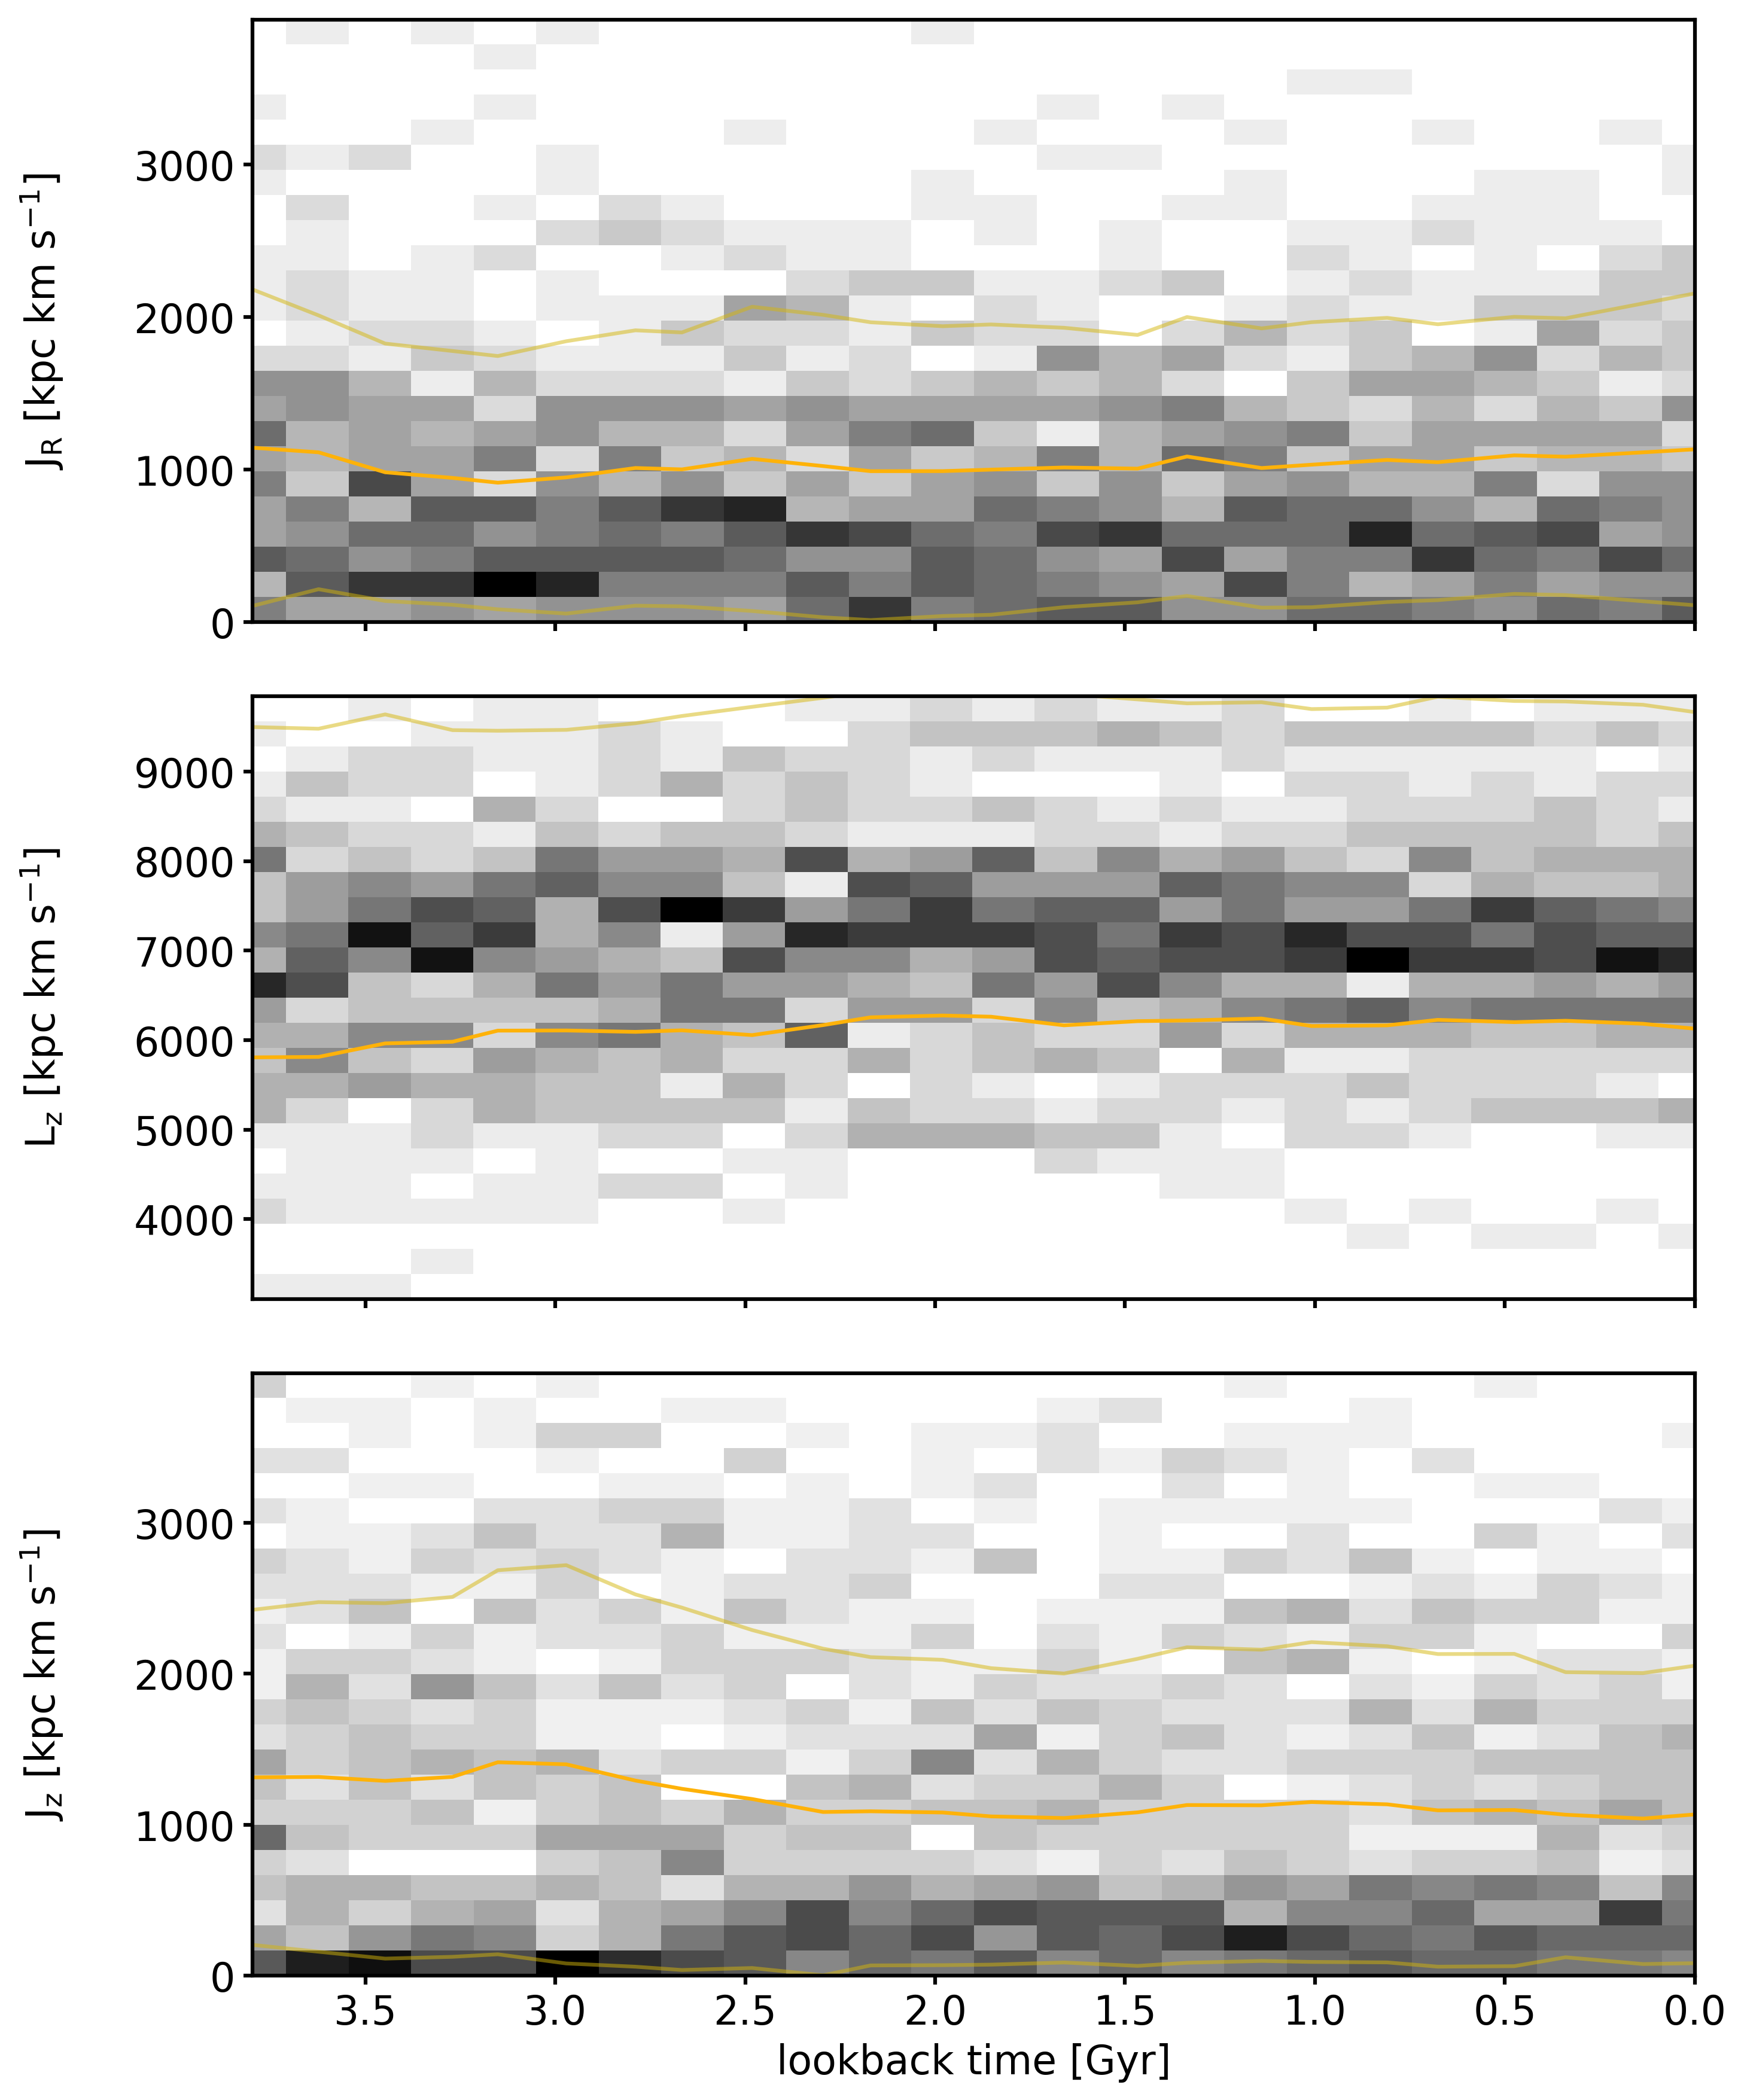
\includegraphics[width=\textwidth]{plots/Dynamics/mean_pot/action_time_evolution_hist_mean_prog4.png}
    \caption{Same as Figure \ref{fig:actions_time_evolution_prog4}, only for a constant potential since the merger of prog2.}\label{fig:actions_time_evolution_mean_pot_prog4}
\end{figure}
\fi

\subsubsection{Energy evolution}\label{subsubsec:energy_evol}
Another assumption under which we calculated the radial and vertical actions were the use of the action estimation method "St\"ackel Fudge". To test if variations and the missing of clumpiness could be due to estimation inaccuracies or numerical problems in this approach we can have a look at the other \ac{IoM}, angular momentum and energy. Since $L_z$ was rather constant in Figures \ref{fig:actions_time_evolution_prog2} - \ref{fig:actions_time_evolution_prog4} and \ref{fig:comparison_actions_time_evolution_mean_pot_prog2} we now evaluate the energy. It is calculated according to Equation \ref{eq:energy_hamiltonian} where $v^2 = \Sigma\limits_{i=1}^3 v_i^2$. We can derive the energy directly from the data by taking the potential value from the simulation. We also compare it to our potential model. The kinematic term of Equation \ref{eq:energy_hamiltonian} is identical for data and model.

\begin{figure}[htbp]
\captionsetup{format=plain}
    \centering
	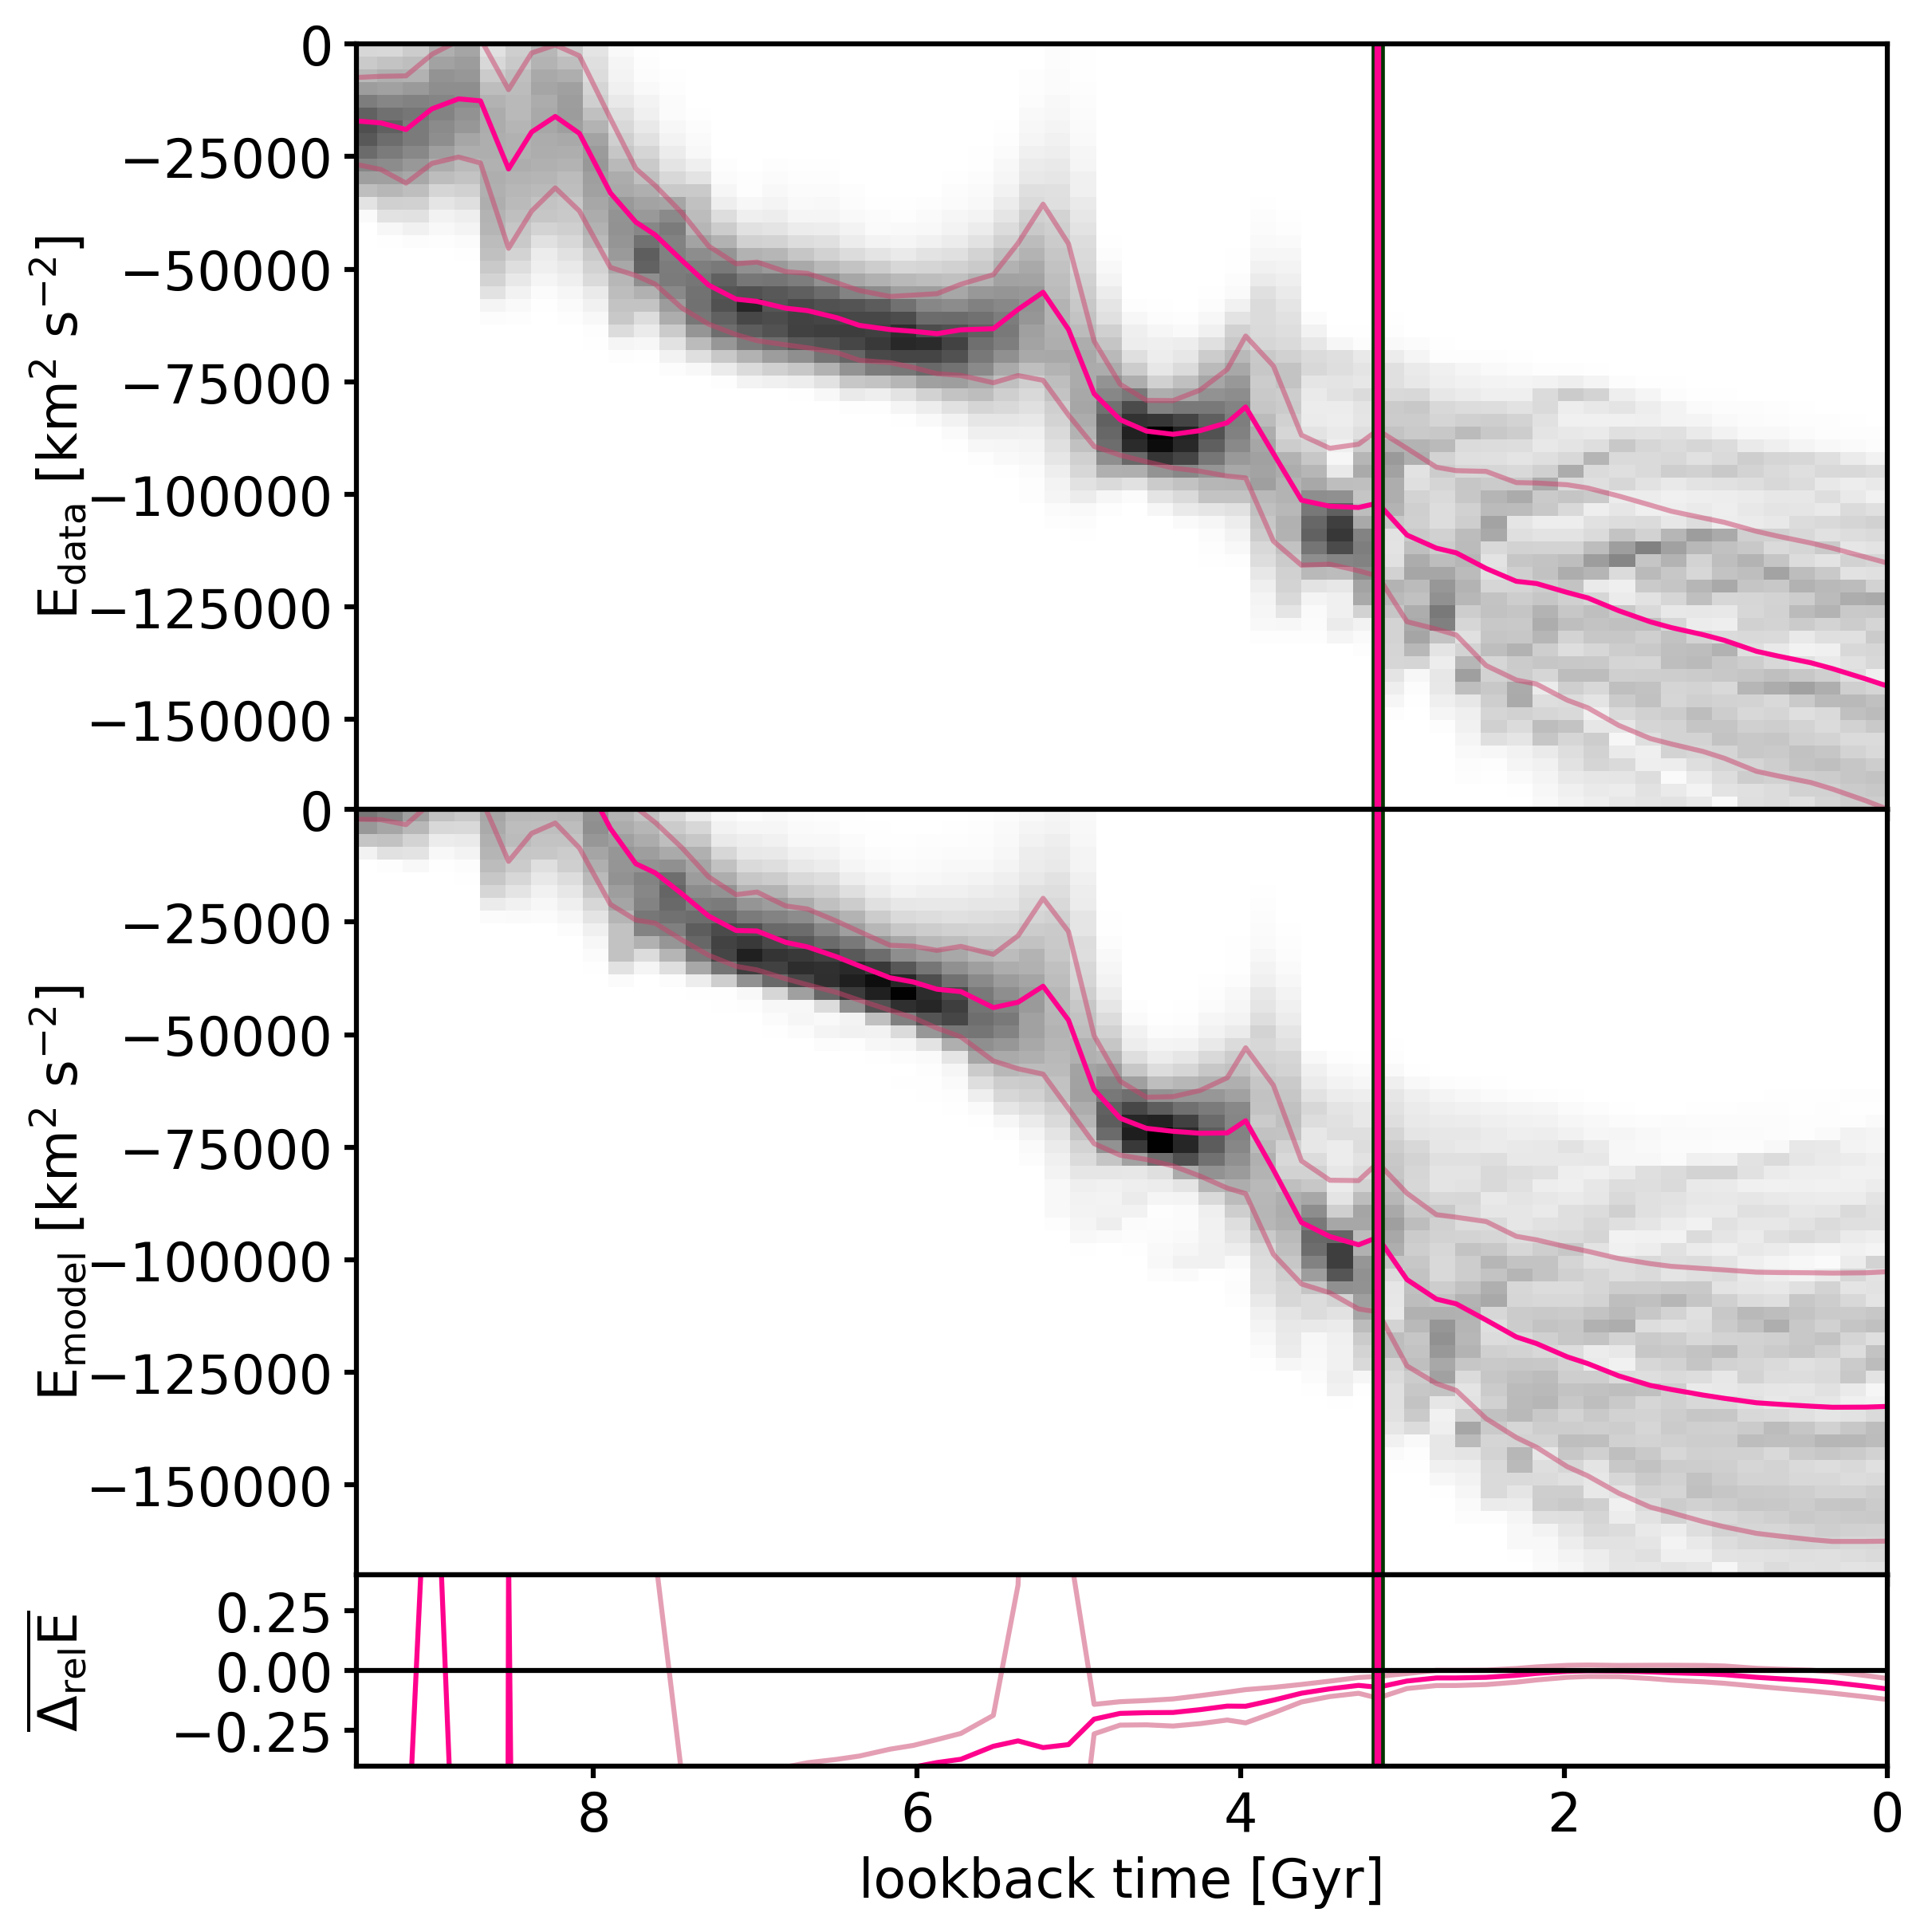
\includegraphics[width=\textwidth]{plots/Dynamics/prog2/energy_time_evolution_gcwodisk_hist_mean.png}
	\caption{Time evolution of the energy of the particles of prog2. \textit{Upper panel}: The true energy, which the particles have according to their kinetic energy and their potential value as returned by the Auriga simulation. \textit{Middle panel}: Energy calculated in the interpolated best fit potential. \textit{Lower panel}: Mean relative error of the energy. The \acp{GC} spiral in and continue to lose energy even after the merger.  }\label{fig:energy_time_evolution_prog2}
\end{figure}

We show the energy evolution in Figure \ref{fig:energy_time_evolution_prog2}. Here it again becomes obvious, that the potential fit could be better since the model overestimates the energy up to a few \SI{10000}{km^{2}.s^{-2}}. Especially before the merger, the relative error is very big (too big to display it). As the \acp{GC} spiral in, the relative error becomes smaller. It seems like the potential fit got better there. The overall trend is still similar. As the \ac{DG} spirals in it falls deeper into the potential well. This trend continues even after the merger. Therefore it still loses energy. We find the same trend for prog3 and prog4. We observe small scale variations in the energy, similarly to what is seen in the actions (best seen in $J_R$ in Figure \ref{fig:actions_time_evolution_prog3}.
\\\\\textcolor{red}{check language}This gives another evidence that within our goal to evaluate the galaxy in an analytic axisymmetric form we do not have problems with our assumptions but it seems that the simulation is just too complex to model it that simply.

\iffalse
\begin{figure}
\captionsetup{format=plain}
    \centering
	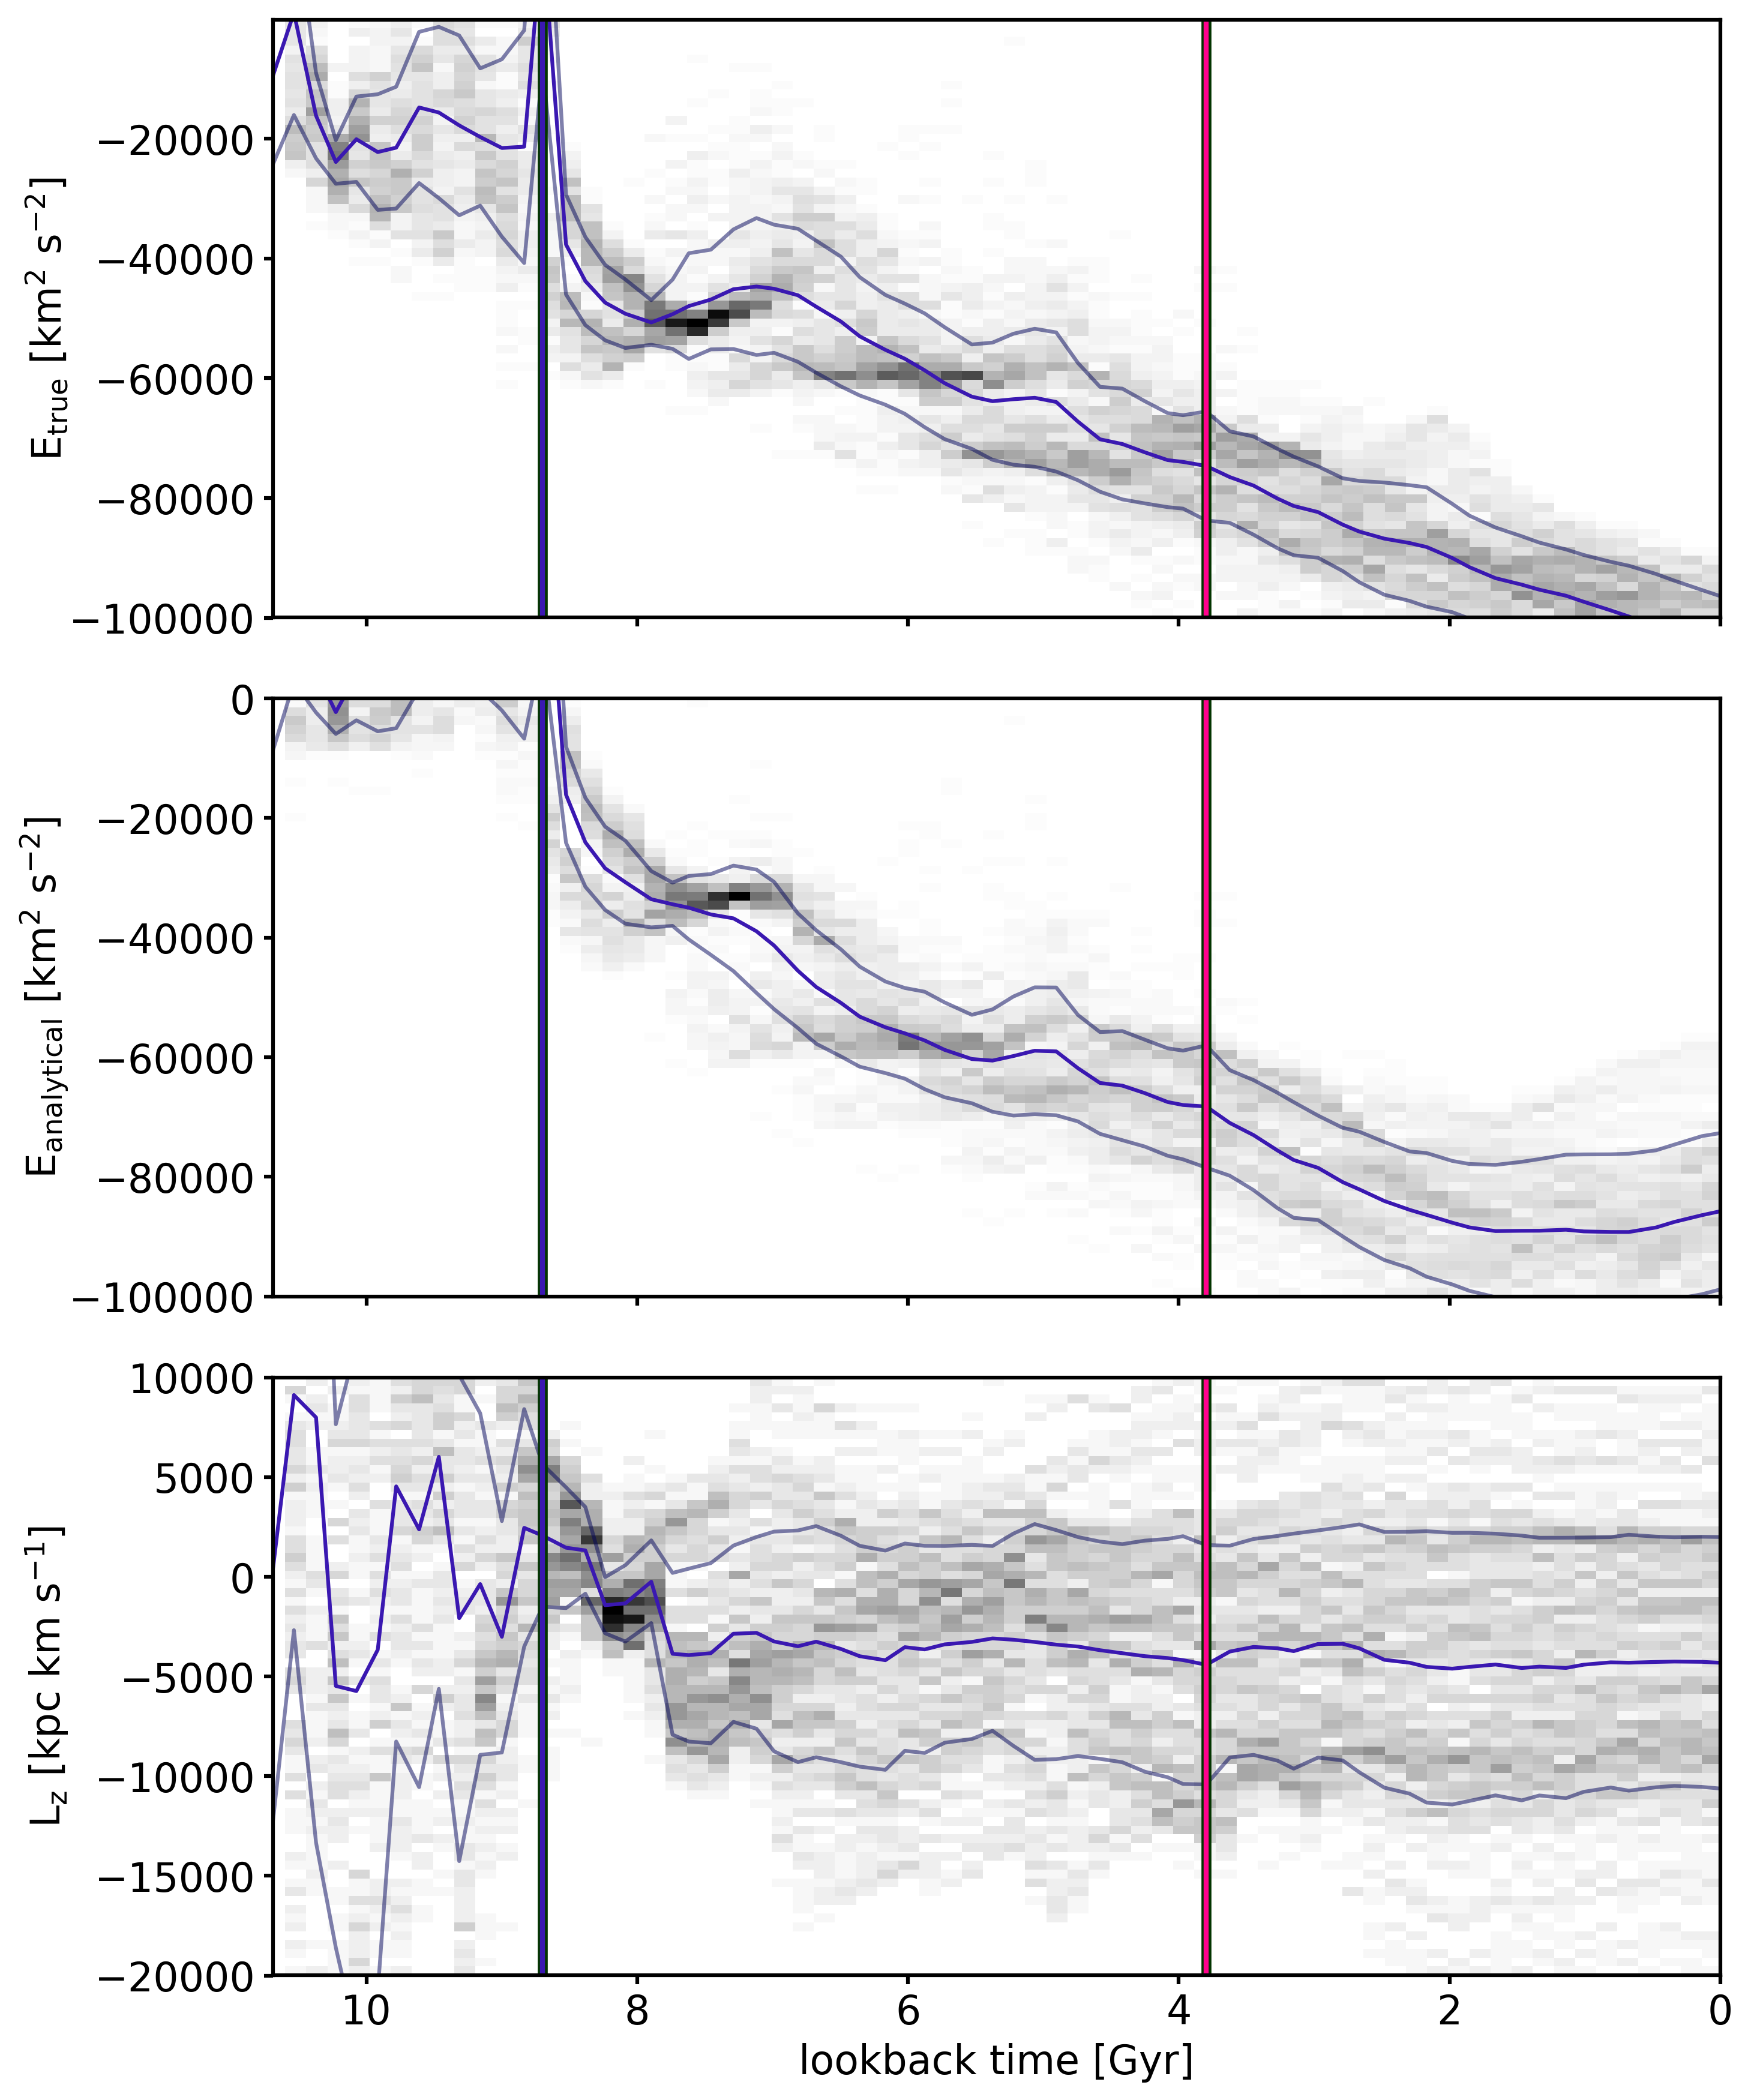
\includegraphics[width=\textwidth]{plots/Dynamics/prog3/energy_time_evolution_hist_mean.png}
    \caption{Same as \ref{fig:energy_time_evolution_prog2} but for prog3. }\label{fig:energy_time_evolution_prog3}
\end{figure}

\begin{figure}[htbp]
\captionsetup{format=plain}
    \centering
	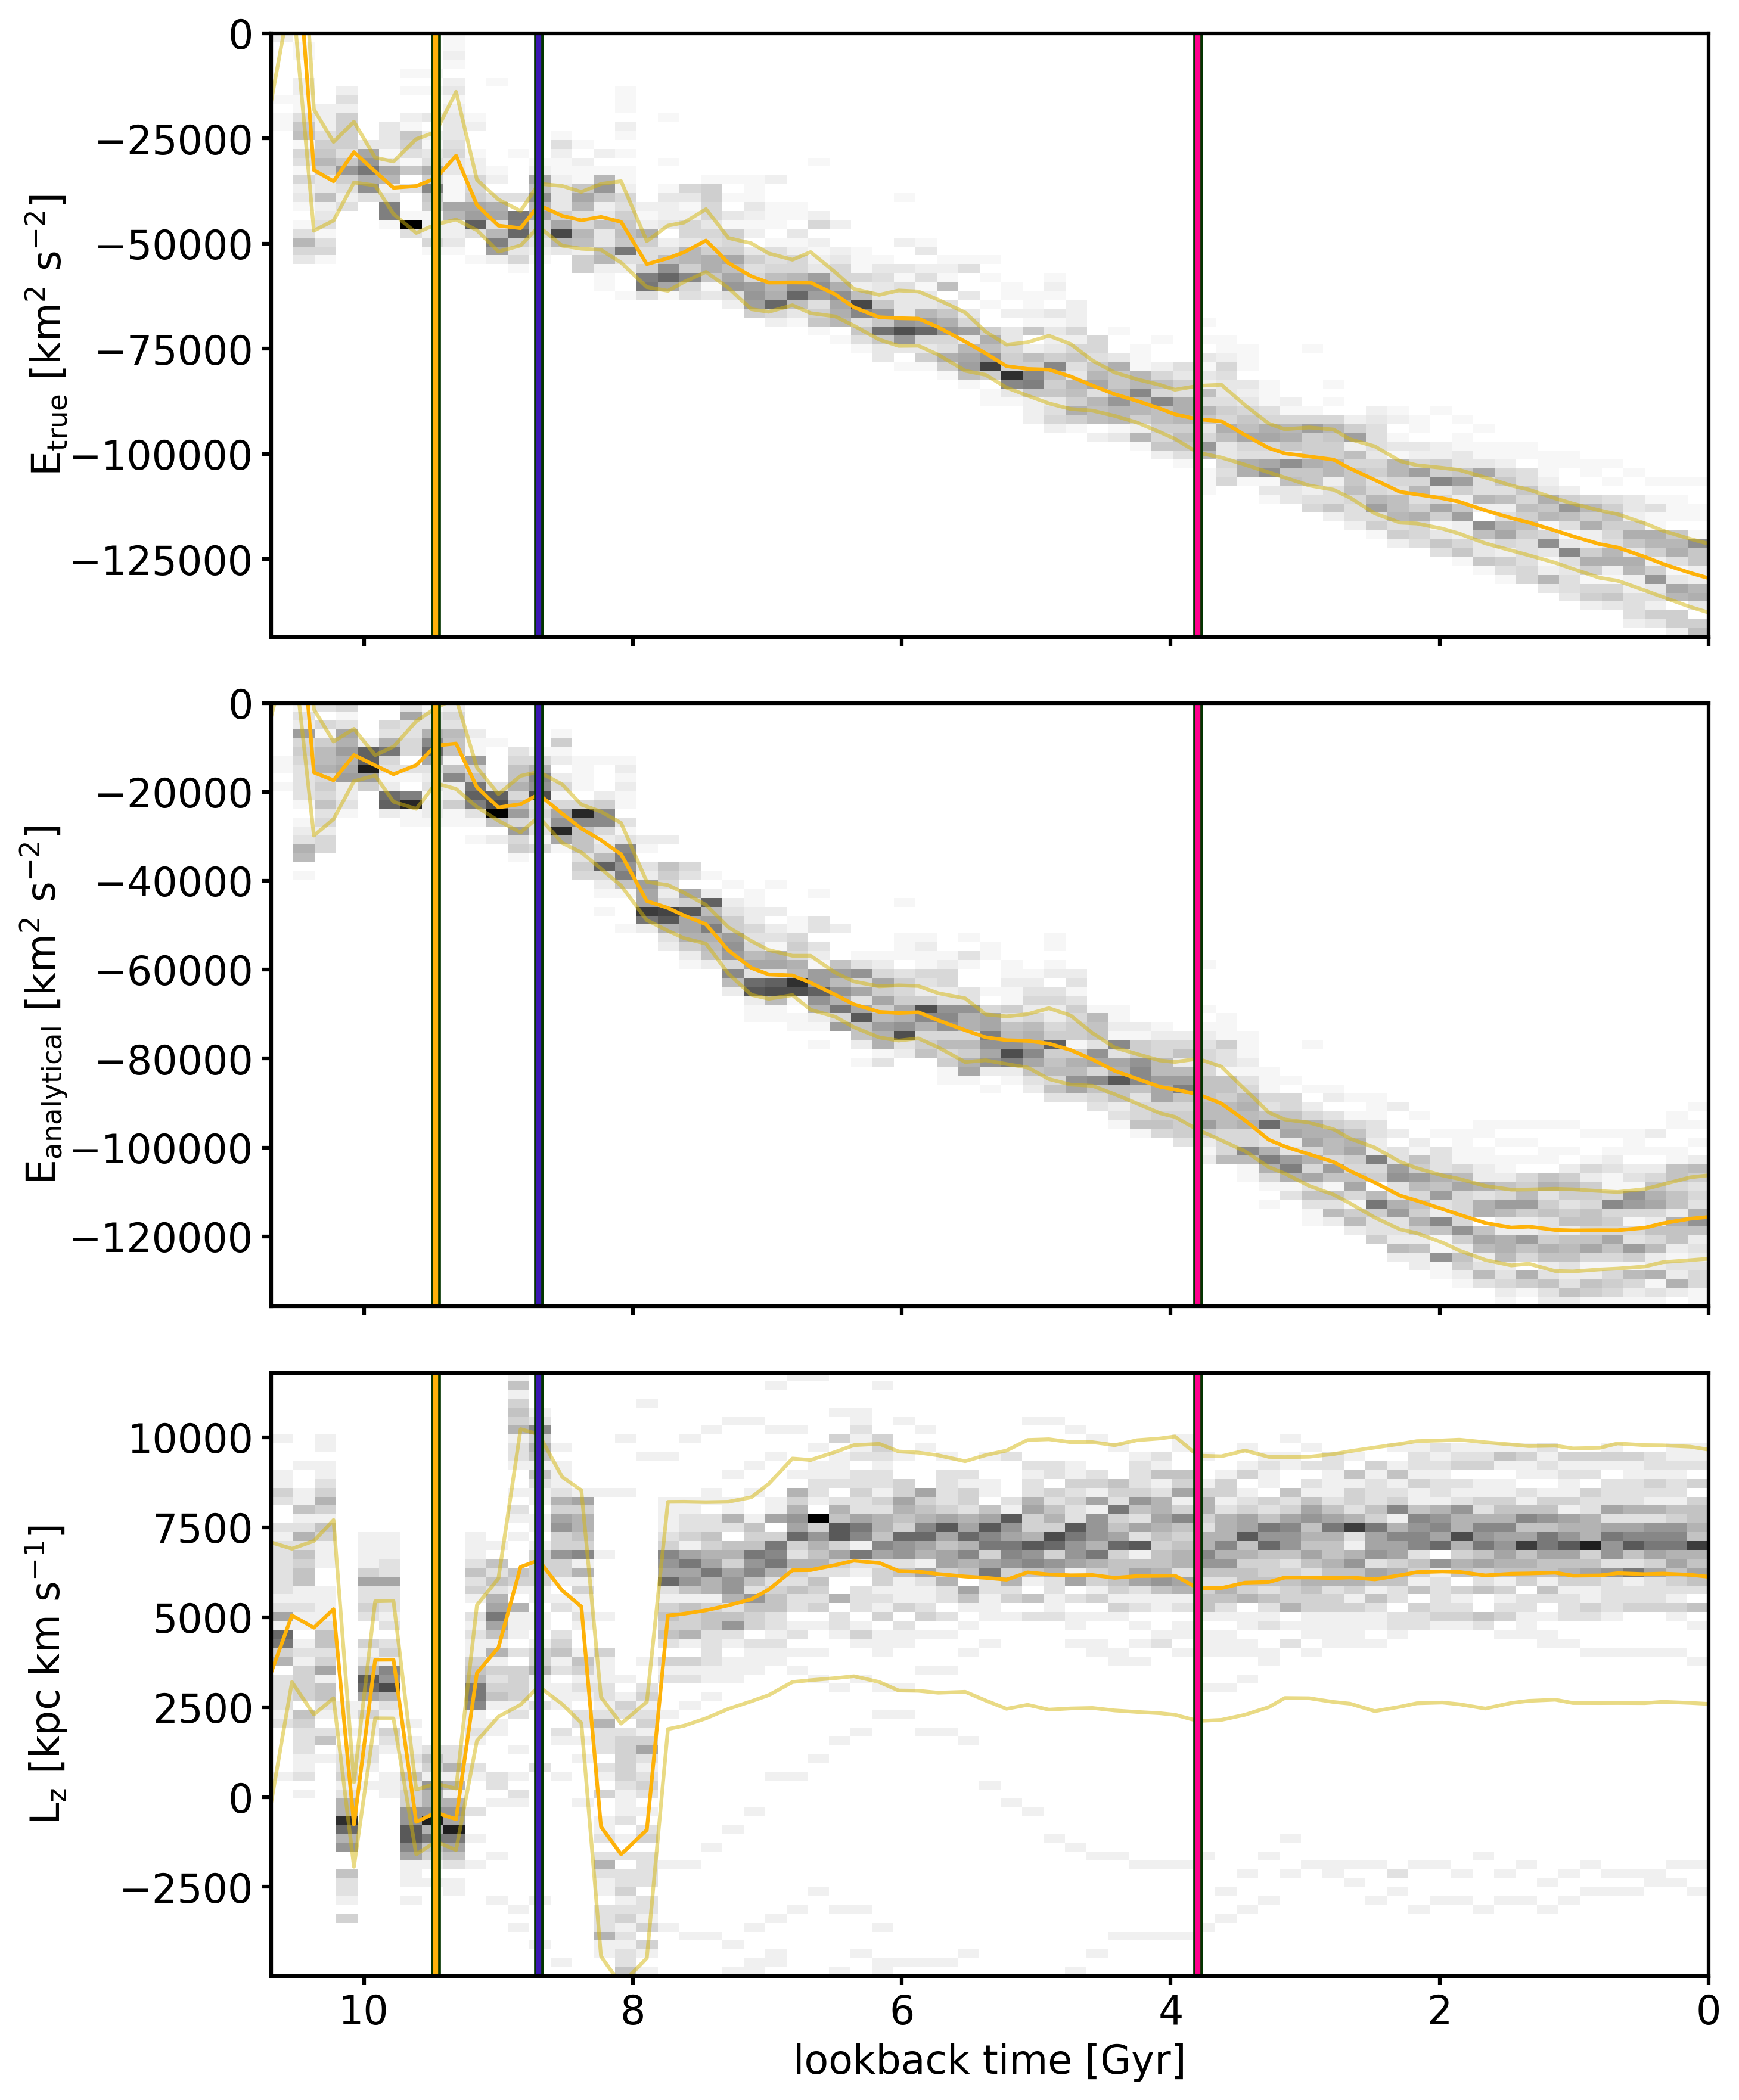
\includegraphics[width=\textwidth]{plots/Dynamics/prog4/energy_time_evolution_hist_mean.png}
    \caption{ame as \ref{fig:energy_time_evolution_prog2} but for prog4.}\label{fig:energy_time_evolution_prog4}
\end{figure}
\fi

\subsection{Test: evolution of globular clusters on same orbit at $z=0$}\label{subsec:box_GCs}
In Section \ref{subsec:GCs_action_space} we found that the overall \ac{GC} distribution in action space is not very clumped. In Section \ref{subsec:time_evo_actions} we saw a rather constant evolution of the actions but with a large scatter. Now we investigate \acp{GC} whose actions are close together in the last snapshot. The selection of these "box \acp{GC}" is made by taking the mean of each action and find all \acp{GC} within a cube centered on the means with a gradually increasing side length. For prog2, we want to look at a larger of 20 particles. To have 20 particles in this cube required a side length of \SI{650}{kpc.km.s^{-1}}. Since we have fewer particles accreted from prog3 and prog4, they needed bigger side lengths and therefore the orbits of their box particles are a priori not as close.  


\begin{figure}[htbp]
\captionsetup{format=plain}
    \centering
    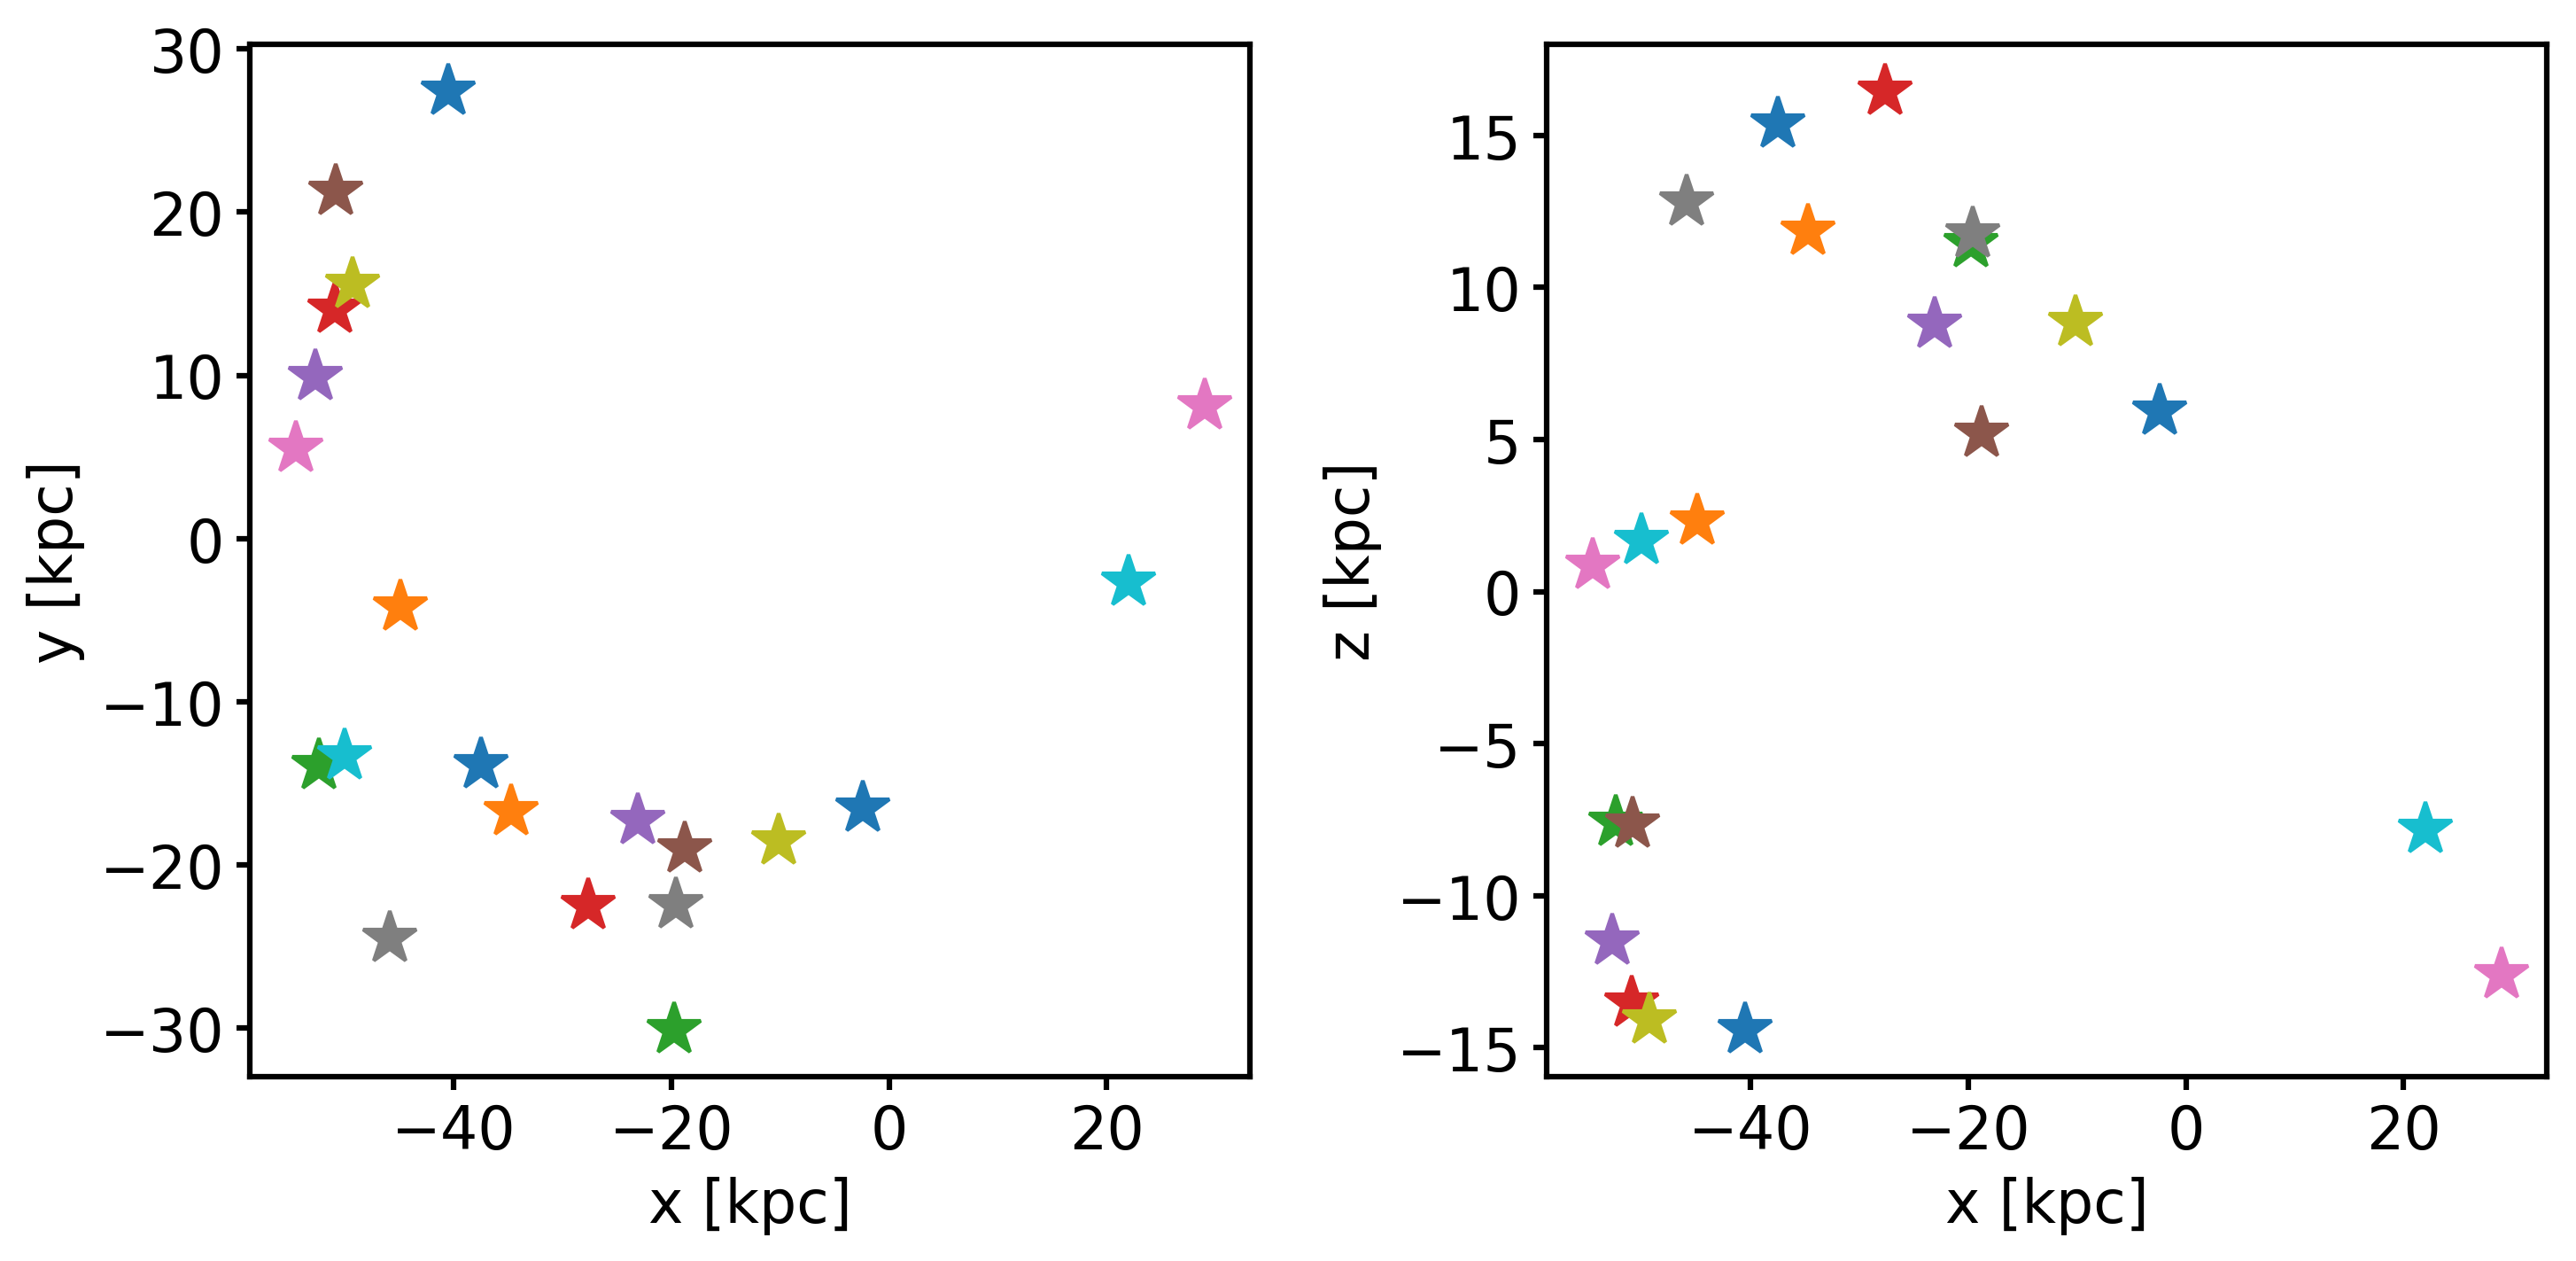
\includegraphics[width=0.9\textwidth]{plots/Dynamics/prog2/gowidsk_progenitor2_box_distribution.png}
    \caption{Spatial distribution of selected box particles. \textcolor{red}{update with new selected GCs and therefore new boxcoming}}
    \label{fig:box_GCs_distr}
\end{figure}

Their spatial distribution is presented in Figure \ref{fig:box_GCs_distr}. There is a small clustering around $x = \SI{50}{kpc}$ but all other selected GCs are well distributed in space. 

\iffalse
\begin{figure}[htbp]
\captionsetup{format=plain}
    \centering
	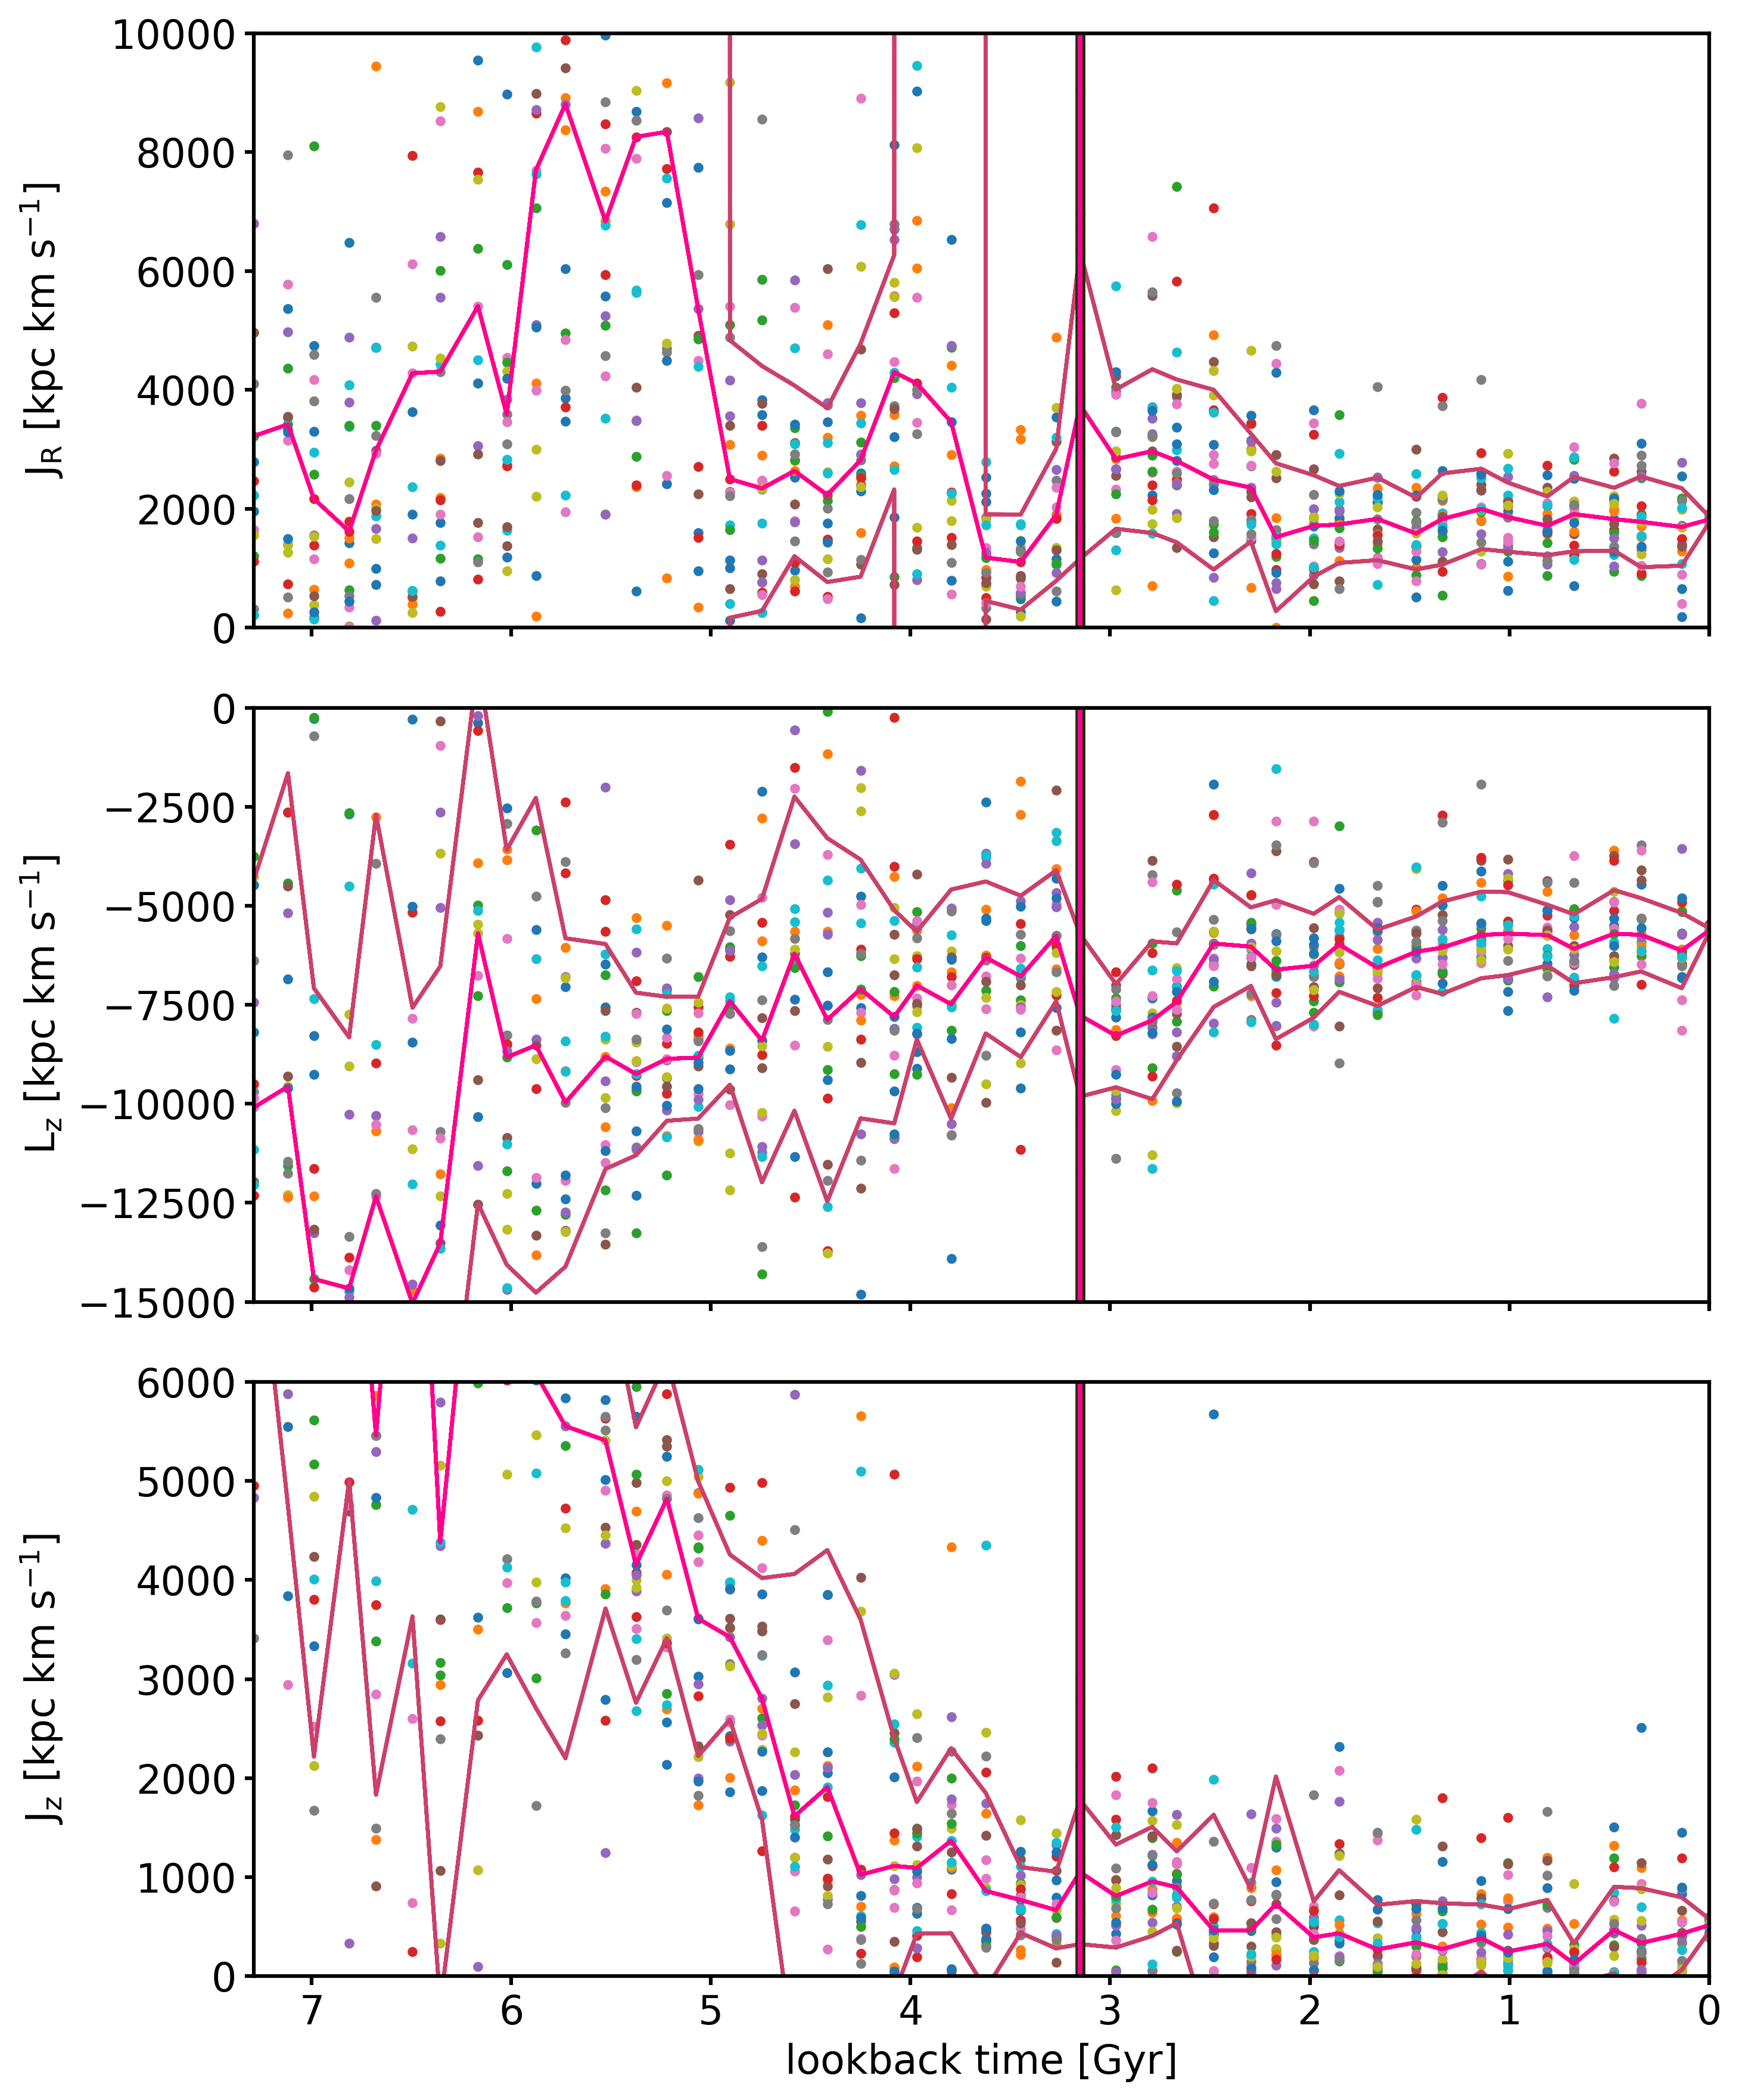
\includegraphics[width=\textwidth]{plots/Dynamics/prog2/gcwodisk_action_time_evolution_box_hist_mean.png}

	\caption{Action time evolution of 17 particles of prog2 which are found to be on similar orbits in the $z=0$ snapshot. \textcolor{red}{update with new selected GCs and therefore new boxcoming} }\label{fig:actions_box_time_evolution_prog2}
\end{figure}
\fi


\begin{figure}[htbp]
\captionsetup{format=plain}
    \begin{subfigure}[c]{0.48\textwidth}
    \centering
    	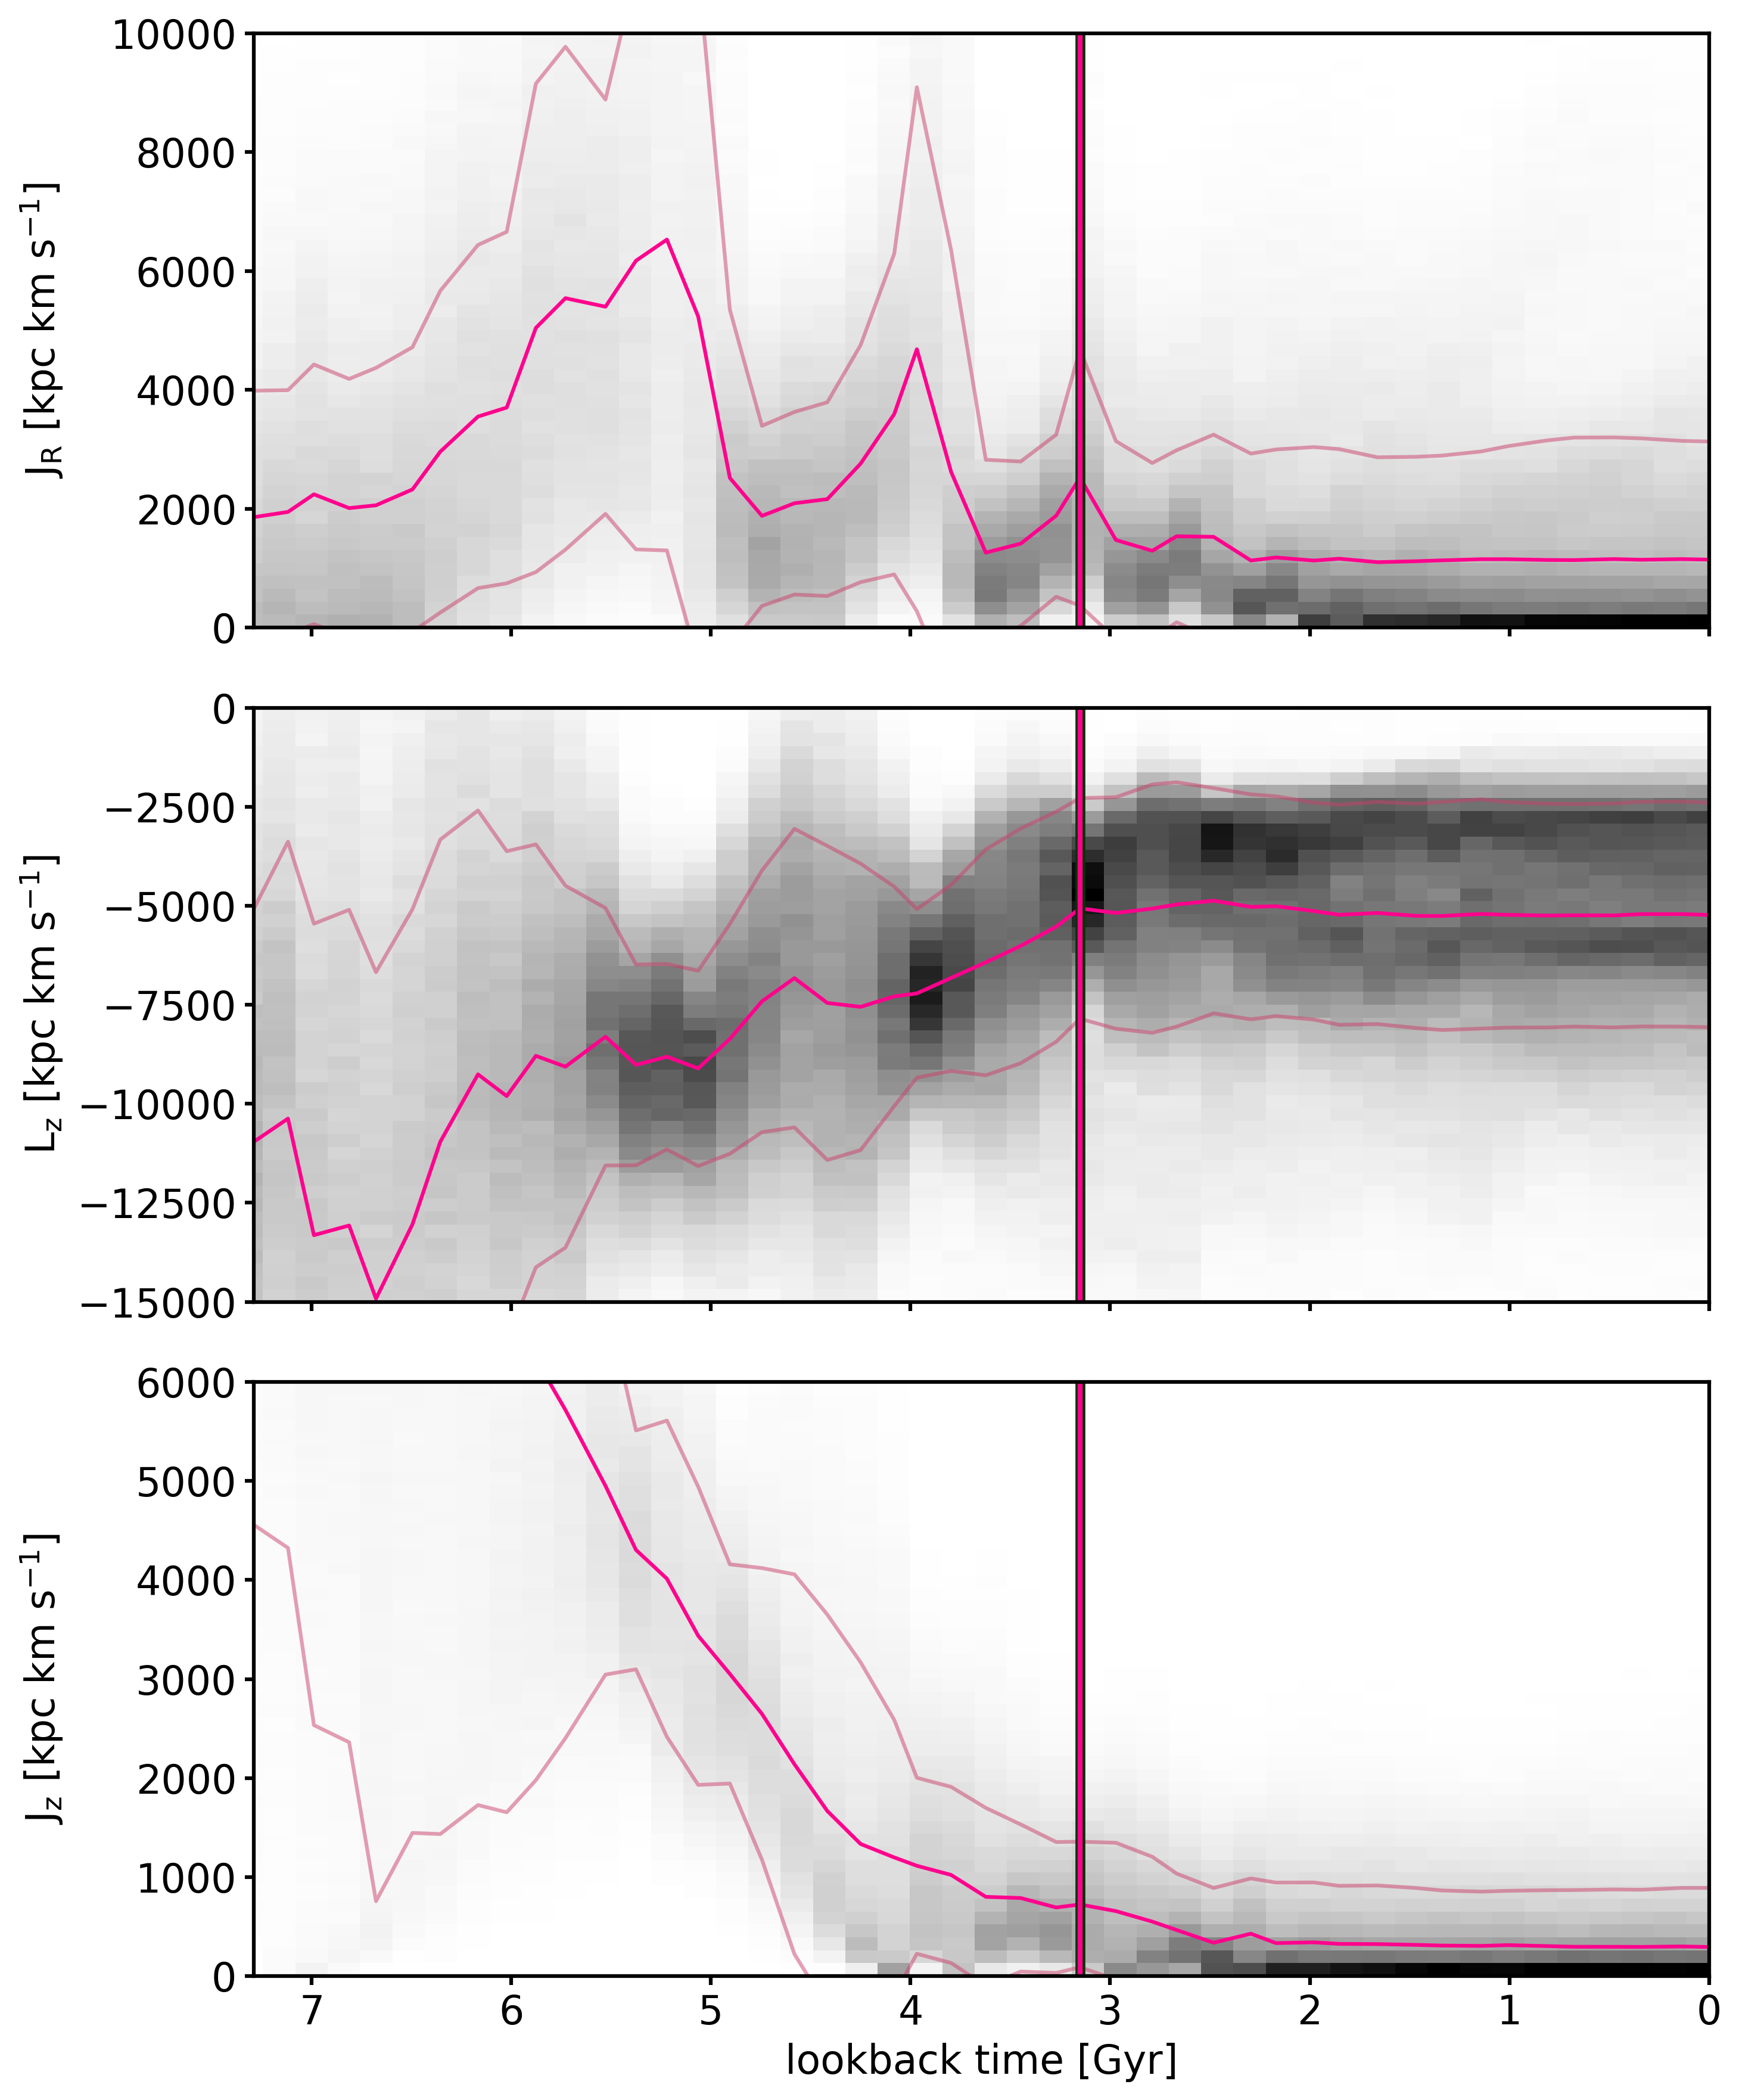
\includegraphics[width=\textwidth]{plots/Dynamics/prog2/action_time_evolution_wodisk_hist_mean.png}
    \end{subfigure}
    ~
    \begin{subfigure}[c]{0.48\textwidth}
    \centering
	    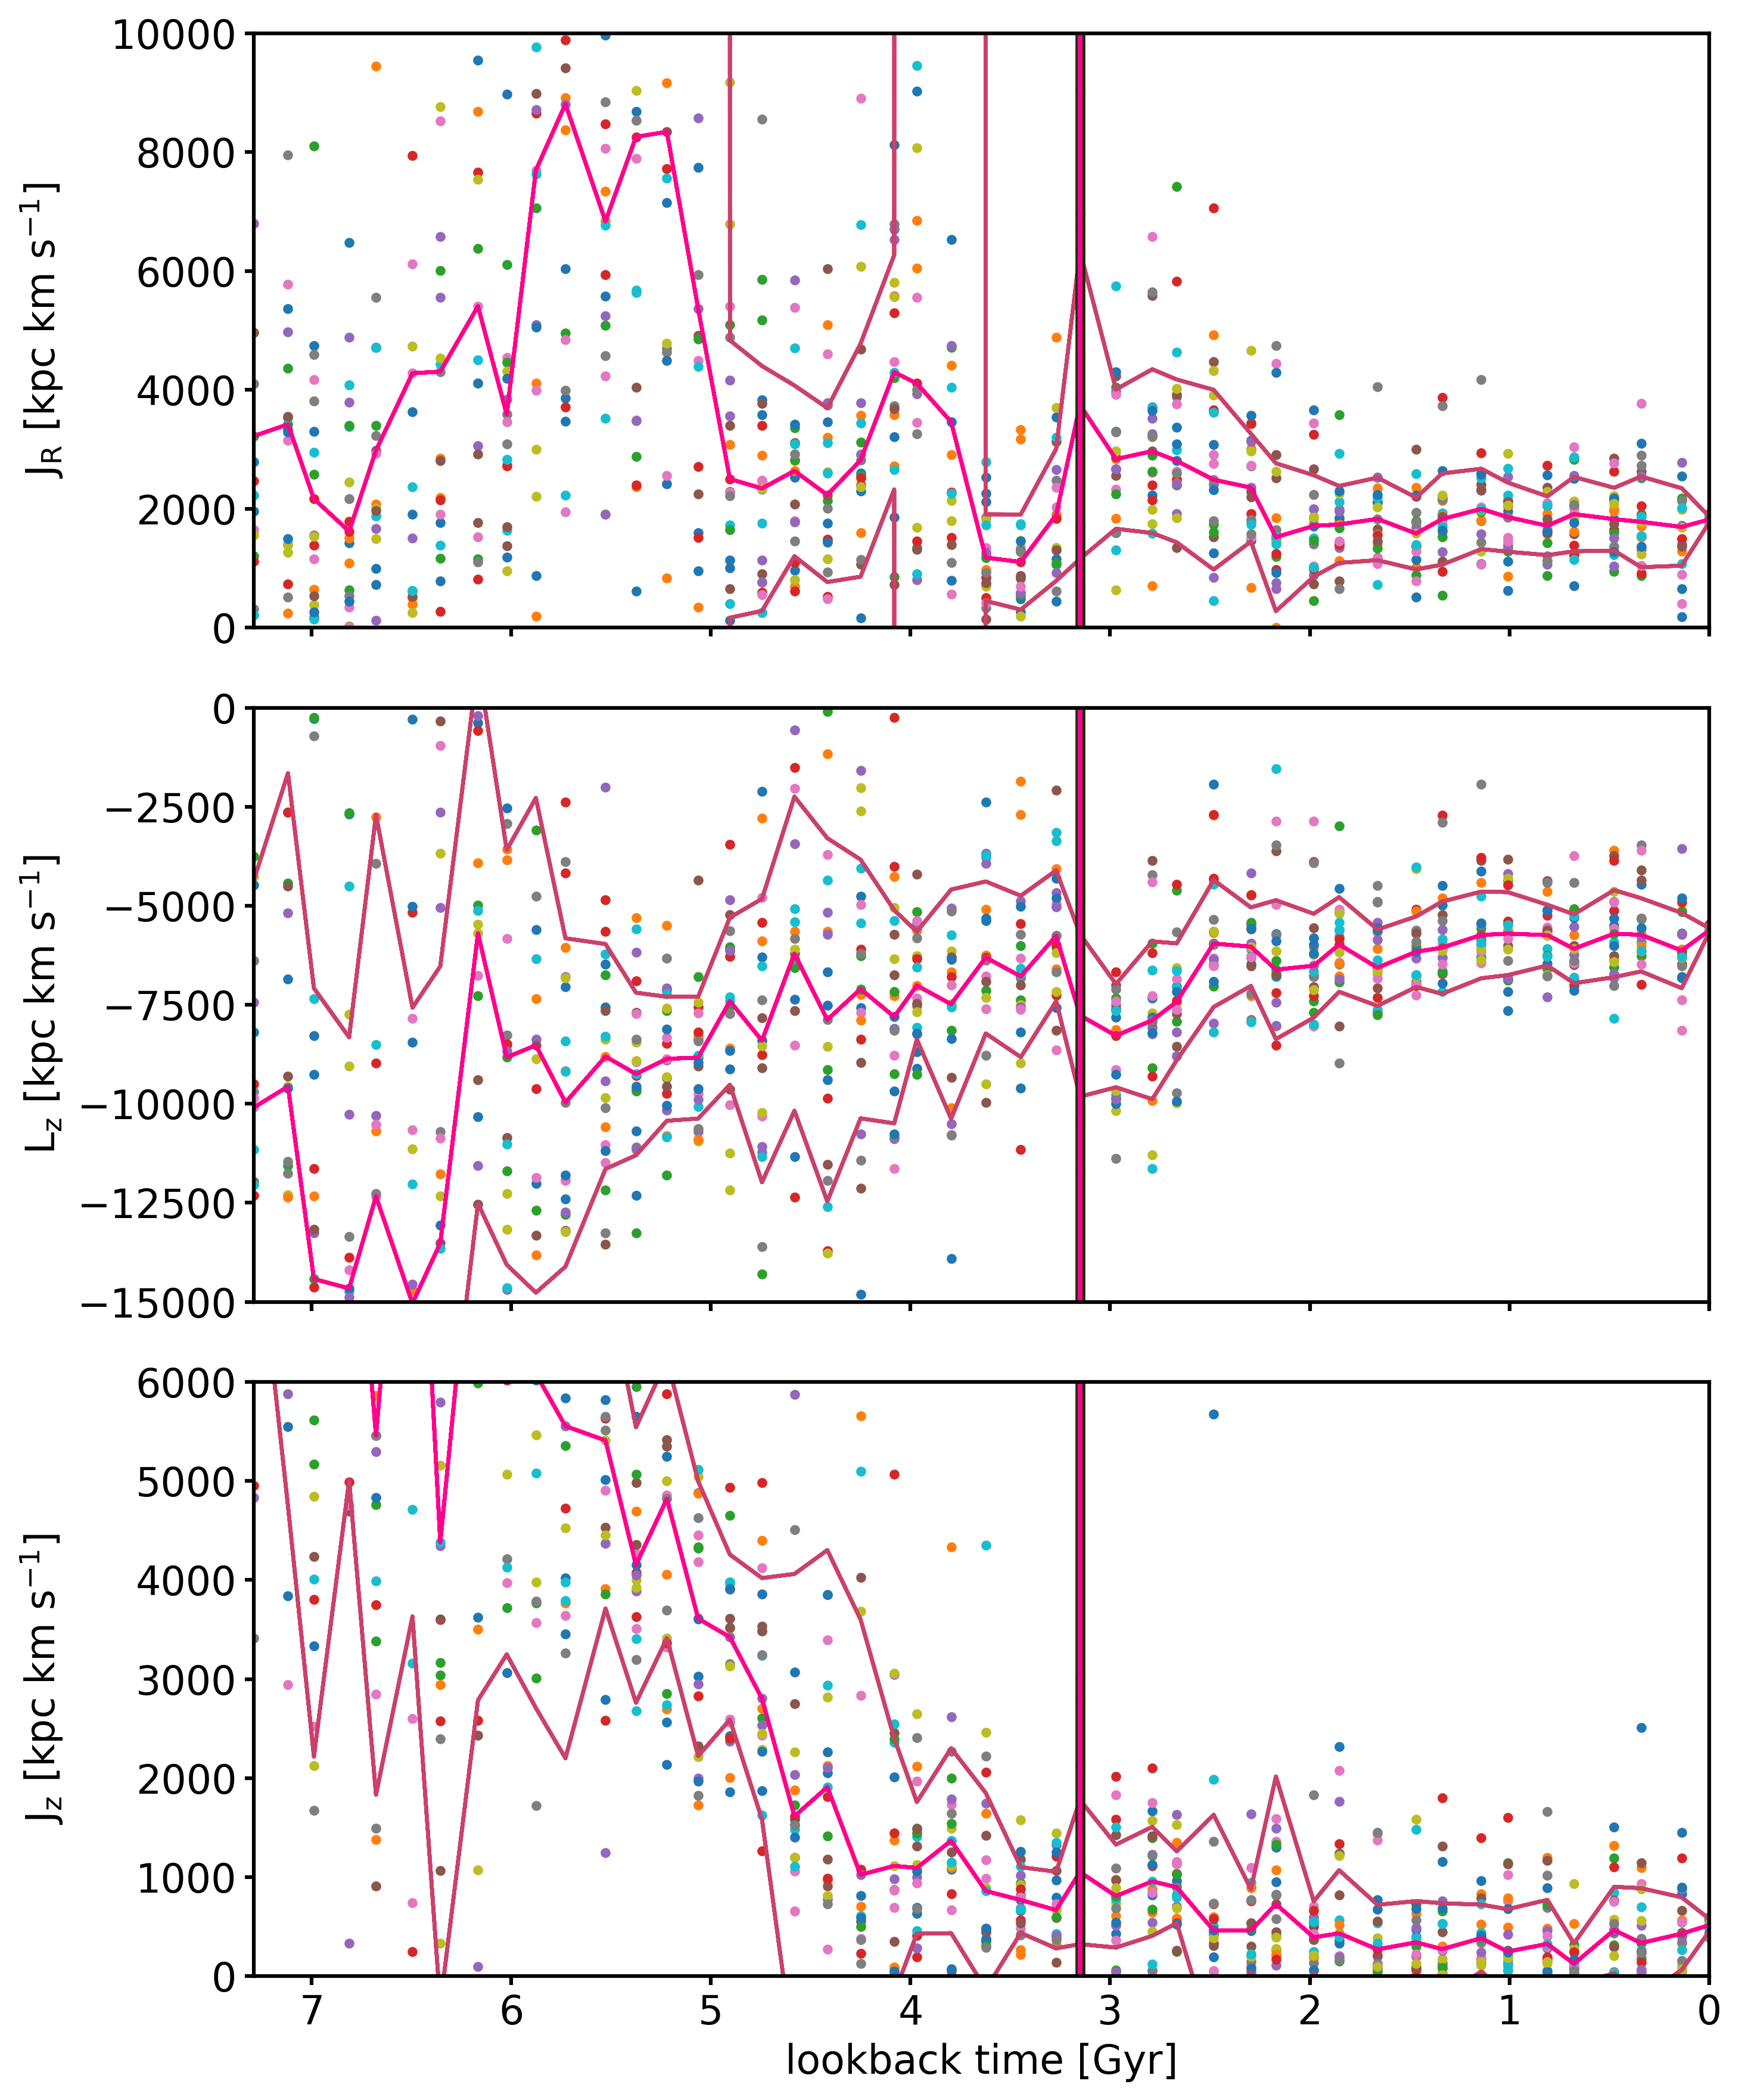
\includegraphics[width=\textwidth]{plots/Dynamics/prog2/gcwodisk_action_time_evolution_box_hist_mean.png}
    \end{subfigure}
    \caption{\textcolor{red}{update with new selected GCs and therefore new boxcoming}}\label{fig:comparison_actions_time_evolution_box_prog2}
\end{figure}
In Figure \ref{fig:comparison_actions_box_time_evolution_prog2}, we plot the evolution of these actions in the right panel. At the last snapshot, we see how close they are in all three actions by construction. But already one snapshot before, they spread out widely and do not have any connection. Going back in time, the spread approximately stays constant. So even though we find similar orbit parameters at the very end, they do not evolve similarly. We compare the evolution of the box particles to the evolution of all accreted particles from prog2 in the left panel. The median and standard deviations evolve around the same values. \\\\
We constructed a case in which we find a few \acp{GC} on similar orbits at the current time as we find them in observations. These could be used to constrain the potential by minimizing their spread. \textcolor{red}{ irgendwie einmal nett formulieren in dieser subsection If we found \acp{GC} clumped together in actions today, they could have a similar evolution or would just be on the same orbit now by chance. }Looking at their time evolution leads to the conclusion that they are only on same orbits right now by chance and will have different properties soon again. So even if constraining the potential by minimizing the spread of accreted \acp{GC} in action would work we need to be careful in the selection of these \acp{GC}.
\iffalse
\begin{figure}
\captionsetup{format=plain}
    \centering
	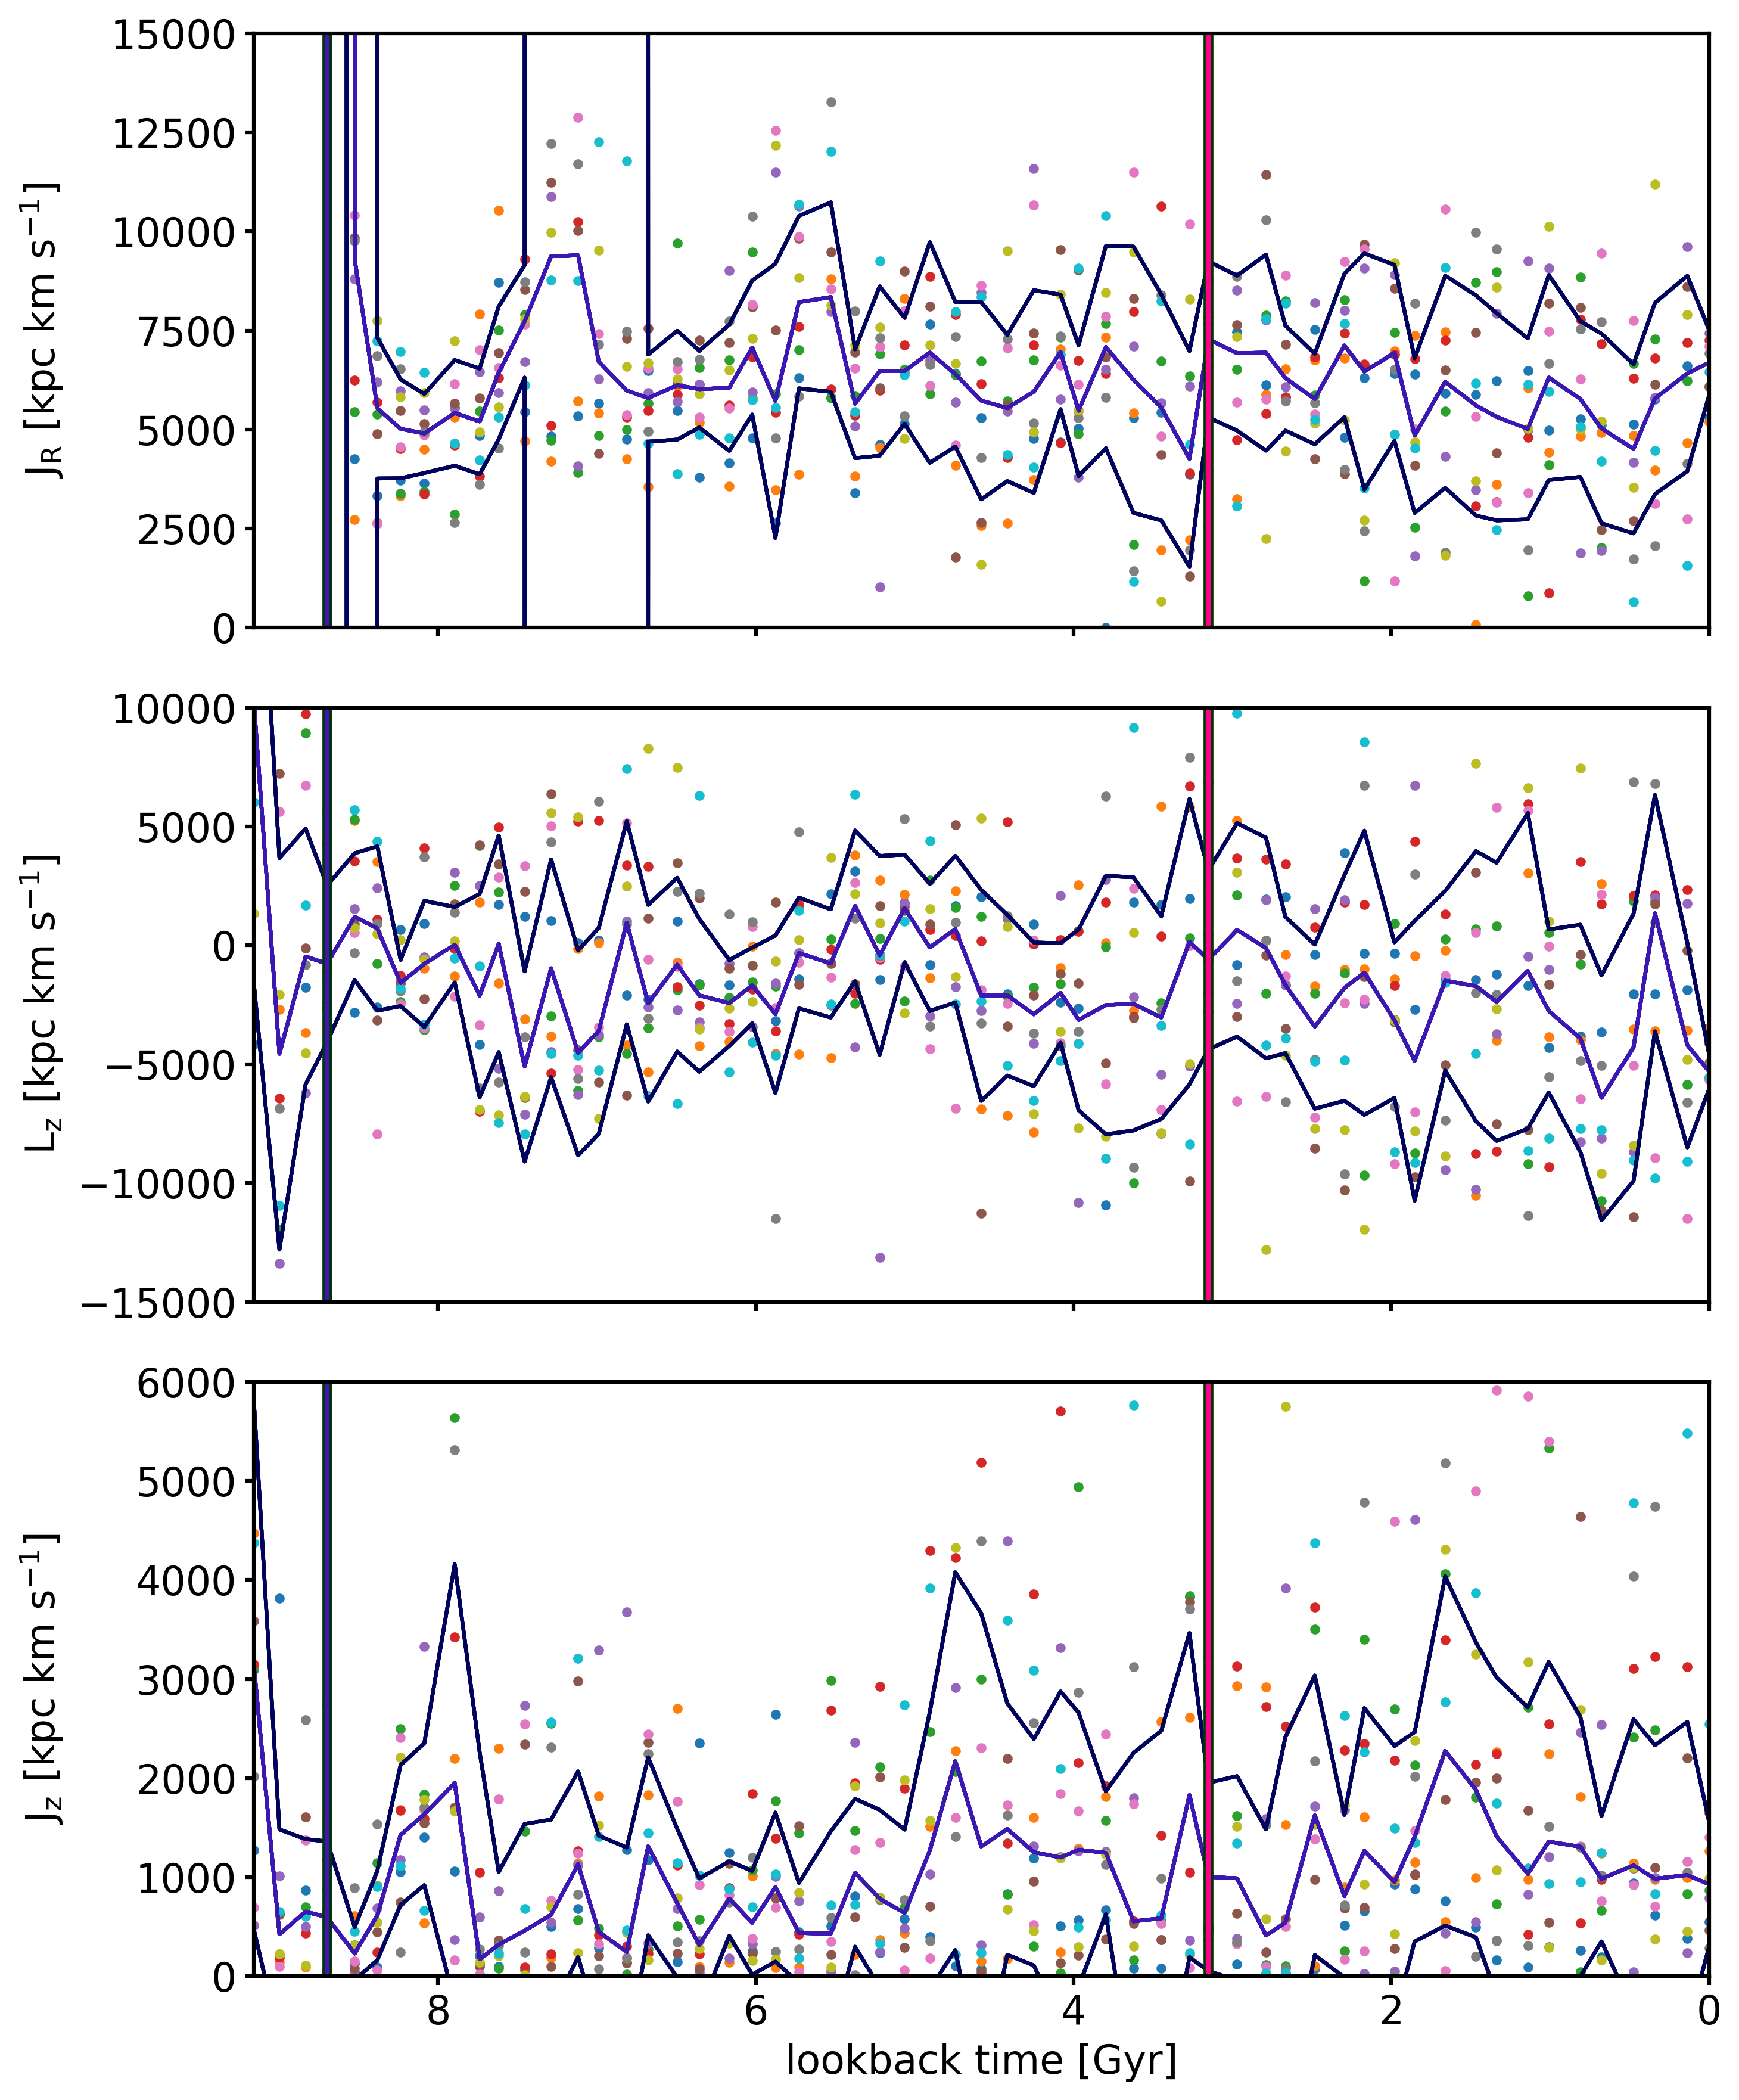
\includegraphics[width=\textwidth]{plots/Dynamics/prog3/action_time_evolution_box_hist_mean_prog3.png}
    \caption{Action time evolution of xx particles of prog3 which are found to be on similar orbits in the $z=0$ snapshot.}\label{fig:actions_box_time_evolution_prog3}
\end{figure}

\begin{figure}[htbp]
\captionsetup{format=plain}
    \centering
	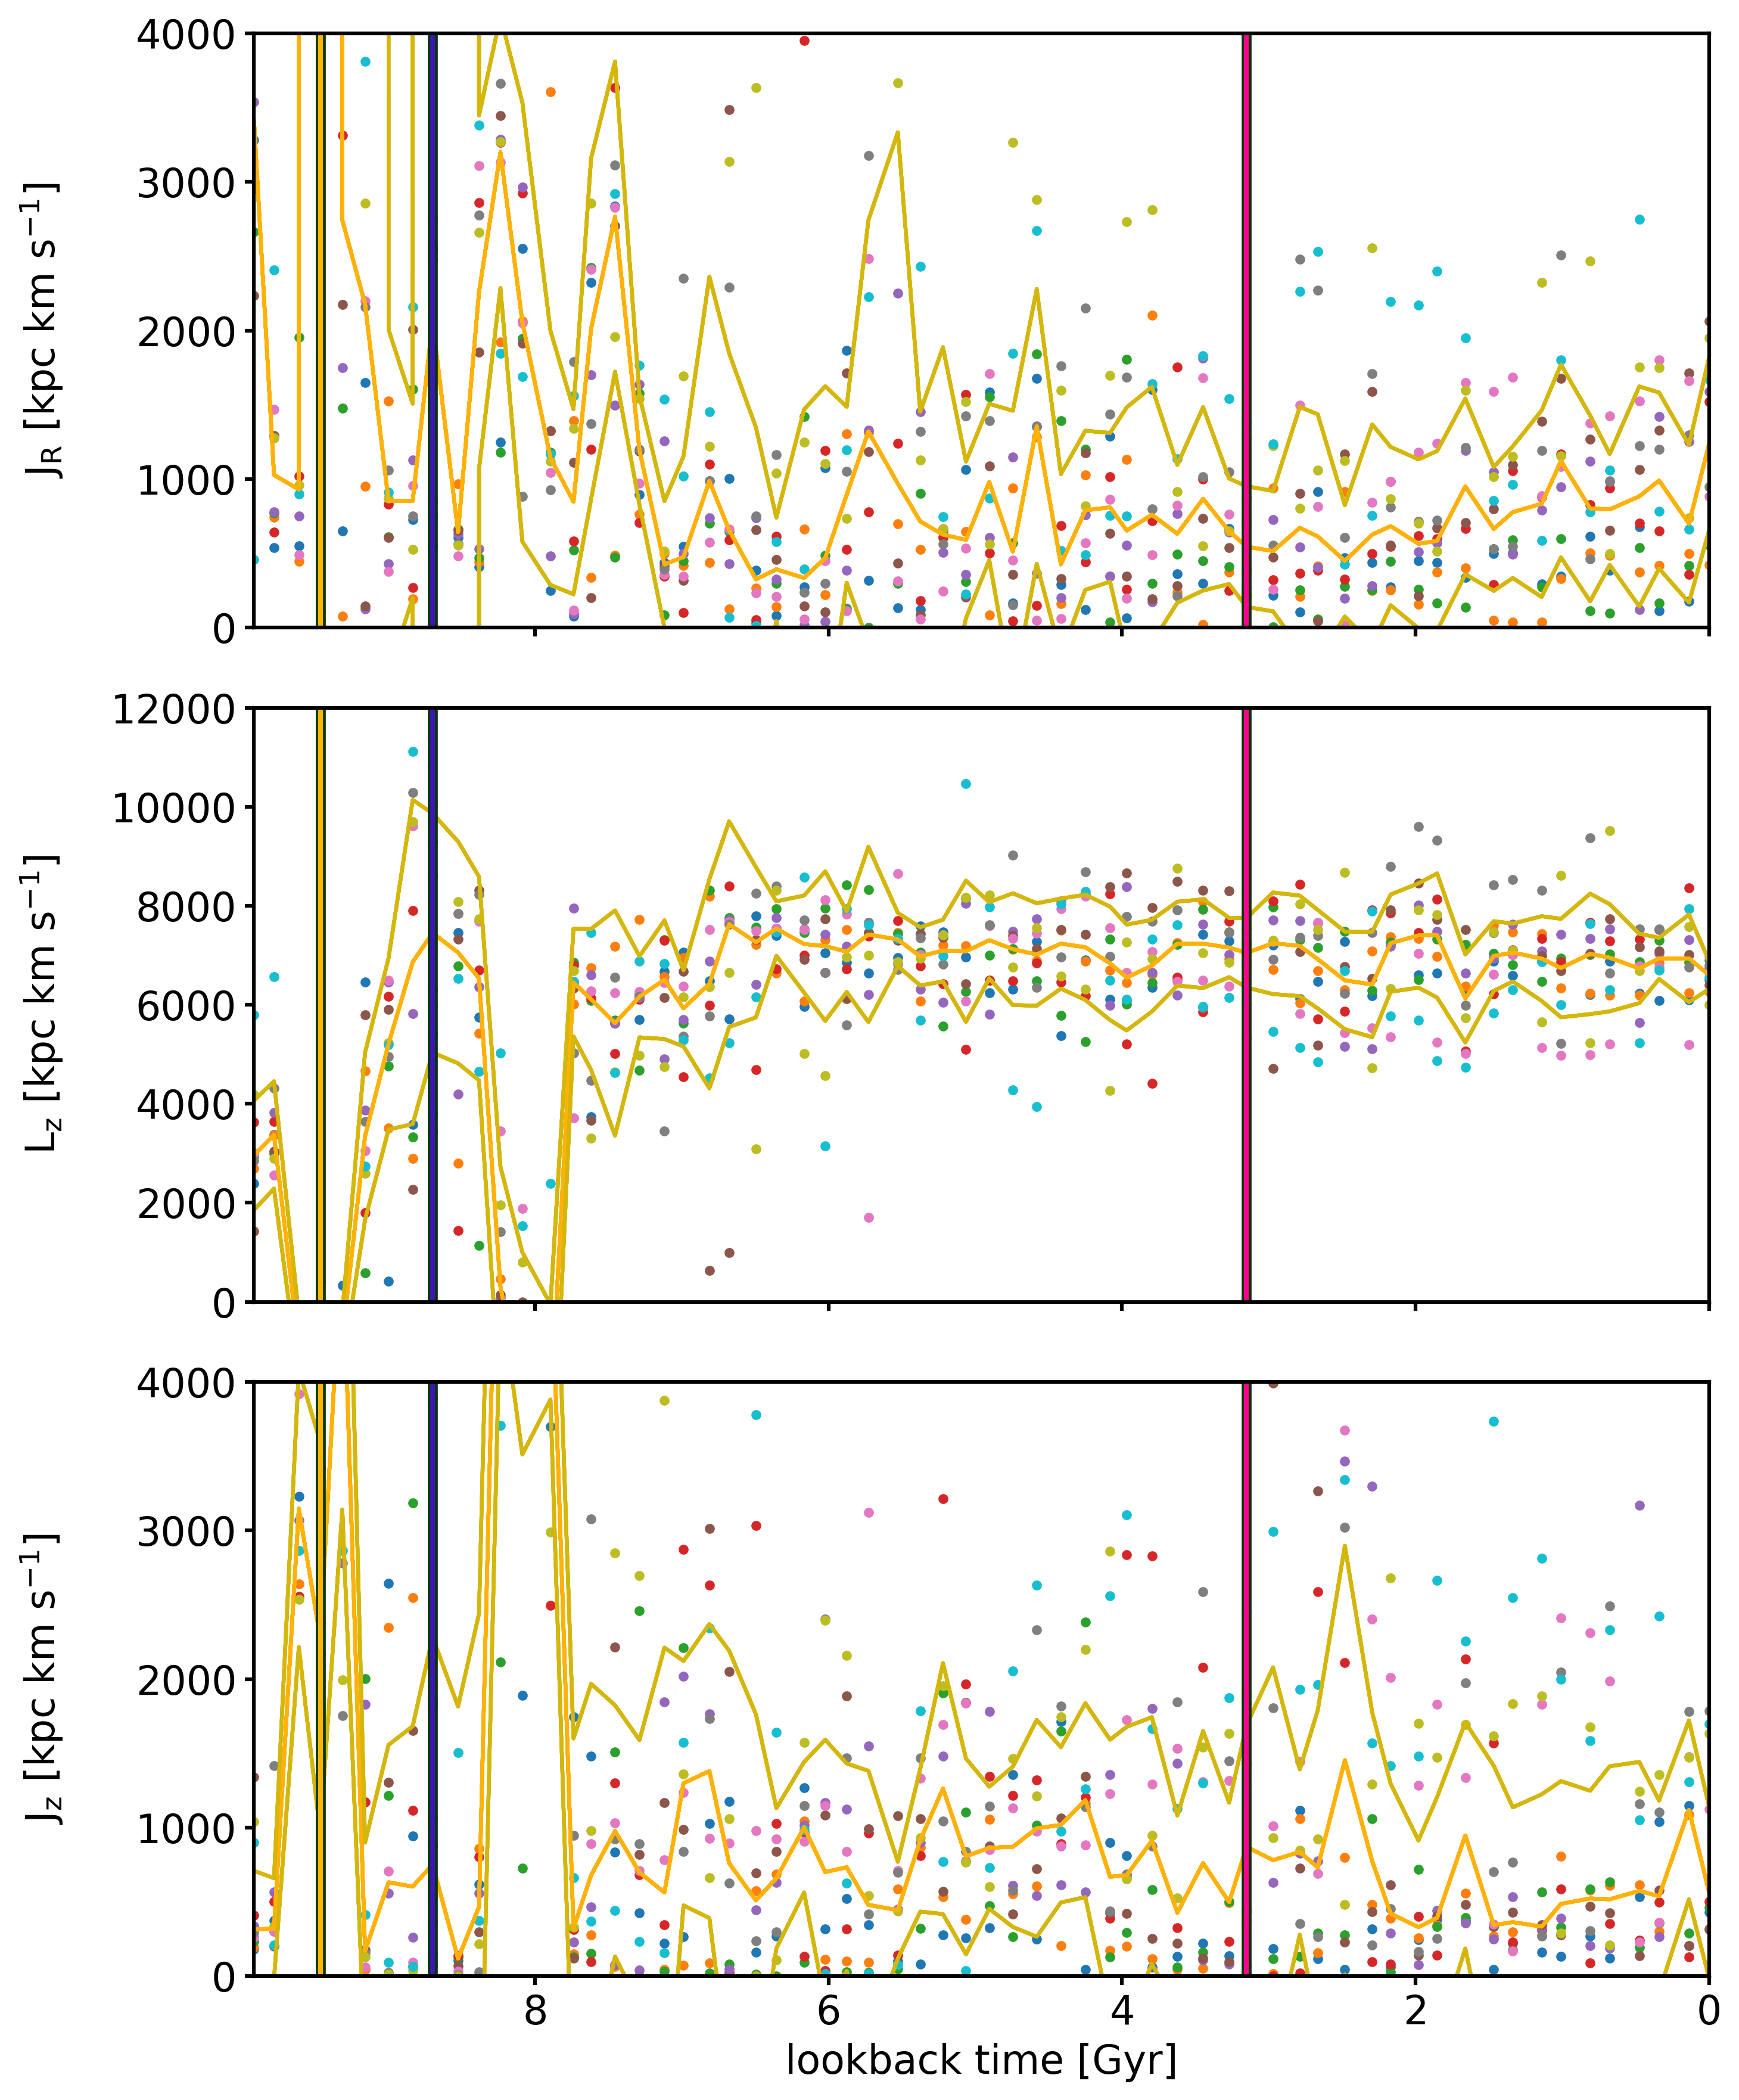
\includegraphics[width=\textwidth]{plots/Dynamics/prog4/action_time_evolution_box_hist_mean_prog4.png}
    \caption{Action time evolution of xx particles of prog4 which are on as similar orbits as possible. }\label{fig:actions_box_time_evolution_prog4}
\end{figure}
\fi

